\PassOptionsToPackage{obeyspaces,spaces}{url} % \codigo conserva los espacios
\documentclass[stu,12pt,biblatex,floatsintext]{apa7}
% --- Idioma y codificación ---
\usepackage[utf8]{inputenc}
\usepackage[T1]{fontenc}
\usepackage[spanish,es-tabla]{babel} % es-tabla: «Tabla» en lugar de «Cuadro» (APA)
\setlength{\parindent}{1.27cm}
\usepackage[table]{xcolor}
% --- Utilidades comunes ---
\usepackage{csquotes}
\usepackage{graphicx}
\usepackage{booktabs}
\usepackage{setspace}
\usepackage{caption}
\usepackage{hyperref} % apa7 ya carga hyperref: sus opciones van en \hypersetup
\hypersetup{colorlinks=true, linkcolor=blue, urlcolor=blue, citecolor=blue,
            hypertexnames=false} % anclas únicas: cada parte reinicia la numeración de secciones
\usepackage{amsmath,amssymb}
\usepackage{array}
\usepackage{tabularx}
\usepackage{float}
\usepackage{pdflscape} % páginas horizontales para diagramas de secuencia
\usepackage{longtable}
\usepackage{enumitem}
\usepackage{tikz}
\usetikzlibrary{arrows.meta, decorations.pathreplacing, positioning, shapes.geometric, shapes.multipart, fit, calc}
\usepackage{minted}
\setminted{breaklines} % las líneas largas de código no se salen del margen
% --- Bibliografía (APA 7) ---
\usepackage[style=apa,backend=biber]{biblatex}
\DeclareLanguageMapping{spanish}{spanish-apa}
% --- Evitar que las notas al pie se dividan entre páginas ---
\interfootnotelinepenalty=10000

\title{Proyecto final: ShiftCash}
\shorttitle{ShiftCash}
\addbibresource{referencias.bib}
\DefineBibliographyStrings{spanish}{
  references = {Bibliografía},
}
\renewcommand{\arraystretch}{1.5}

% --- Caracteres de los guiones incluidos que pdfLaTeX no trae ---
\DeclareUnicodeCharacter{2500}{-}
\DeclareUnicodeCharacter{1F354}{\textit{(icono)}}
\DeclareUnicodeCharacter{1F4BC}{\textit{(icono)}}
\DeclareUnicodeCharacter{1F3AC}{\textit{(icono)}}

% --- Convenciones propias del documento ---
\setcounter{secnumdepth}{3} % secciones numeradas para poder referenciarlas
\renewcommand{\notelabel}{Nota} % apa7 escribe «Note» por defecto
\graphicspath{{images/}}
% Paleta: negro, gris y un solo color de acento
\definecolor{acento}{HTML}{1F4E79}
\definecolor{gris}{gray}{0.45}
\definecolor{grisclaro}{gray}{0.88}
% Datos que debe aportar el equipo (lista final: grep -rn "pendiente" secciones/)
\newcommand{\pendiente}[1]{\textbf{[PENDIENTE: #1]}}
% =====================================================================
% RESULTADOS QUE APORTA EL EQUIPO
% Este es el único archivo que hay que editar después de las pruebas con
% usuario y de repetir las herramientas. Cada valor aparece en todas las
% secciones que lo usan. Reemplace el texto entre llaves del \newcommand.
% =====================================================================

% ---------------------------------------------------------------------
% 1. Prueba de aceptación (Segunda parte, sección 6; Apéndice G)
% ---------------------------------------------------------------------
\newcommand{\resUsuarioFinal}{Gonzalo Nicolas Morales Ciriza, usuario externo al equipo}
\newcommand{\resFechaSesion}{25/11/2026}
\newcommand{\resCommitDesplegado}{la rama \codigo{main} después de integrar \codigo{fix/defectos}}
\newcommand{\resCasosEjecutados}{17 de 17}
\newcommand{\resCasosAceptados}{17 aceptados y 0 rechazados}
\newcommand{\resRFAceptados}{20/20 = 100\,\%}
\newcommand{\resObservaciones}{(1) «La primera vez que abrí la página en el celular tardó en cargar»; (2) «Después de un rato sin usarla, el resumen tardó unos segundos en mostrar los datos»; (3) «Sería útil que la última categoría que usé apareciera primero al registrar un gasto»}
\newcommand{\resAcciones}{(1) mejora futura: bajar el LCP en perfil móvil (Tercera parte, eficiencia de desempeño); (2) mitigada: es D-09, con el aviso «Despertando el servidor» y el ping programado a \codigo{/salud}; (3) mejora futura: se agrega al backlog como historia de usuario}
\newcommand{\resConcepto}{Aceptado con observaciones}
\newcommand{\resActa}{\IfFileExists{images/firma_usuario.png}{diligenciada y firmada digitalmente}{\pendiente{firma digital del usuario final en images/firma\_usuario.png}}}

% ---------------------------------------------------------------------
% 2. Tarea cronometrada PU-06 (Segunda parte, 5.3; Tercera parte, usabilidad)
% ---------------------------------------------------------------------
\newcommand{\resPUParticipantes}{Leonel Garrido Naeder, Edimes Amaya Ballestas, Sabrina Ferreira Ferreira y Gonzalo Nicolas Morales Ciriza, usuarios externos al equipo, e Isabella Amaya, integrante del equipo}
\newcommand{\resPUMediana}{36}
\newcommand{\resPUExito}{5/5 = 1,00}
\newcommand{\resPUObservaciones}{tiempos de 24, 33, 36, 41 y 52 s; dos participantes buscaron primero la categoría «Alimentación» antes de escribir el monto y ninguno pidió ayuda}

% ---------------------------------------------------------------------
% 3. Herramientas que se pueden repetir en vivo (por defecto, el texto
%    dice que no se repitieron; si las corren, reemplazar por el resultado)
% ---------------------------------------------------------------------
\newcommand{\resZapApi}{26/11/2026: 0 altas, 1 media (respuesta 500 con contraseñas de más de 72 bytes, límite de bcrypt; hallazgo abierto), 4 bajas, 116 reglas superadas}
\newcommand{\resZapFrontend}{26/11/2026: 0 altas; las 3 medias iniciales quedaron corregidas y aparecen 6 medias que piden endurecer la CSP (\codigo{unsafe-inline}, comodín), SRI y CORS; 4 bajas; 57 reglas superadas}
\newcommand{\resZapResumen}{0 / 6 (26/11/2026)}
\newcommand{\resSonar}{26/11/2026, Community 26.11: Quality Gate aprobado; seguridad A (0), mantenibilidad A (63), fiabilidad D (110: 103 del frontend, sobre todo reglas de accesibilidad y estilo); cobertura 95,4\,\% en \codigo{backend} y 0\,\% en \codigo{frontend/src} (37,8\,\% global); duplicación 0,5\,\%}
\newcommand{\resSonarLoc}{11\,000 aprox. (26/11/2026)}
\newcommand{\resJmeterRender}{no se ejecutó contra Render porque la API no respondía el 21/11/2026}
\newcommand{\resLambdaEscritorio}{no verificados (se agotaron las sesiones gratuitas de LambdaTest)}
\newcommand{\resLambdaMovil}{no verificados en dispositivos reales}
\newcommand{\resNavegadores}{2/4 = 0,50 (Edge y Safari sin verificar)}
\newcommand{\resDisponibilidadApi}{la API dejó de responder porque Supabase pausó la base por inactividad; el 25/11/2026, al reactivarla, volvió a responder. Desde entonces el ping llama a \codigo{/salud}, que también consulta la base}
\newcommand{\resPIcincoPostgres}{no ejecutado sobre PostgreSQL; verificado en SQLite con las claves foráneas activadas}
 % resultados que aporta el equipo (prueba de usuario y herramientas)
% Nombres de archivos, clases y endpoints del código
\newcommand{\codigo}[1]{\nolinkurl{#1}} % admite cortes de línea en / y _
% Columnas de tabla con ajuste de línea
\newcolumntype{L}[1]{>{\raggedright\arraybackslash}p{#1}}
\newcolumntype{Y}{>{\raggedright\arraybackslash}X}
% Estilos TikZ comunes a los diagramas
\tikzset{
  caja/.style={draw, rectangle, align=center, inner sep=4pt, font=\footnotesize},
  cajagris/.style={caja, fill=grisclaro},
  cajaacento/.style={caja, draw=acento, very thick},
  flecha/.style={-{Stealth[length=2mm]}, thin},
  flechapunteada/.style={-{Stealth[length=2mm]}, thin, dashed},
}

\begin{document}
\begin{titlepage}
    \centering
    % --- Encabezado institucional ---
    \textsc{\large Universidad Popular del César}\\[0.2cm]
    \textsc{\normalsize Facultad de Ingeniería de Sistemas}\\[0.15cm]
    \textit{\textbf{SS602}: Ingeniería de Software II}
    % --- Línea separadora ---
    \rule{\textwidth}{0.6pt}
    % --- Actividad y título ---
    {\Large \bfseries Proyecto final: ShiftCash\par}
    \vspace{0.2cm}
    {\normalsize Aplicación web para el control de finanzas personales\par}
    \vspace{0.5cm}
    \rule{\textwidth}{0.6pt}
    \vspace{3cm}
    % --- Autores ---
    {\large Isabella Amaya\par}
    \vspace{0.2cm}
    {\large Brayan Vásquez\par}
    \vspace{1.5cm}
    {\normalsize Docente: Maribel Romero\par}
    \vfill
    % --- Pie de portada ---
    {\normalsize Valledupar, Cesar\par}
    \vspace{0.1cm}
    {\normalsize \today\par}
\end{titlepage}

\tableofcontents
\newpage

% ===================== PRIMERA PARTE =====================
\part*{Primera parte: análisis y diseño}
\addcontentsline{toc}{part}{Primera parte: análisis y diseño}
% =====================================================================
% Primera parte – 1. Problema y contexto
% =====================================================================
\section{Problema y contexto}

\subsection{Planteamiento del problema}

\paragraph{Quién tiene el problema.} Personas que manejan su propio dinero —estudiantes universitarios con ingresos de mesadas o trabajos de medio tiempo, y trabajadores jóvenes con un salario fijo o ingresos variables— y que necesitan saber en qué se les va el dinero, si respetan los límites que se proponen y cuánto avanzan hacia una meta de ahorro.

\paragraph{Dónde ocurre.} En el manejo diario de las finanzas personales en Colombia. Nuestro contexto inmediato es la comunidad universitaria de Valledupar (Cesar), donde formulamos y probamos la solución.

\paragraph{Cómo ocurre hoy.} Quien intenta controlar sus finanzas lo hace de tres formas: lo apunta en un cuaderno, lleva una hoja de cálculo o confía en la memoria y en el extracto del banco. Las tres tienen el mismo problema: cada gasto se anota a mano, la suma por categoría y el porcentaje consumido de un presupuesto se calculan aparte, los gastos que se repiten (arriendo, suscripciones, salario quincenal) hay que volver a escribirlos cada vez y una meta de ahorro no se traduce en un plan concreto de cuánto guardar cada día. El extracto bancario solo muestra los movimientos de una cuenta y no los clasifica según los rubros de la persona. El resultado es que el registro se abandona o queda incompleto.

\paragraph{Evidencia.} La Encuesta de Medición de Capacidades Financieras de 2019, aplicada a 12\,000 hogares, encontró que solo el 51\,\% de los encuestados hace un presupuesto para manejar sus ingresos y gastos, y solo el 47\,\% anota sus gastos de manera regular \parencite{asobancaria2021}. Es decir, \textbf{más de la mitad de las personas (53\,\%) no lleva un registro regular de sus gastos} y casi la mitad (49\,\%) no tiene presupuesto. La misma fuente señala que el índice de educación financiera de Colombia retrocedió 1,13 puntos frente a la medición de 2013 de la CAF.

Para el contexto local, \pendiente{resultados de la encuesta o entrevista del equipo: número de personas, cómo registran hoy sus gastos, cuántas abandonaron el registro y por qué}.

\paragraph{Qué queda fuera del problema.} No abordamos la gestión de inversiones ni de créditos, la contabilidad de empresas o negocios, la declaración de impuestos, la conexión automática con cuentas bancarias ni el asesoramiento financiero. Tampoco pretendemos resolver la falta de educación financiera en sí: la reconocemos como causa, pero nuestra solución se dirige a la herramienta de registro y control (ver la sección \ref{sec:causas}).

\subsection{Causas y efectos}\label{sec:causas}

La Figura \ref{fig:arbol} resume el árbol de problemas. El problema central es que \emph{las personas no llevan un control sistemático de sus ingresos, gastos y metas de ahorro}.

\begin{figure}[H]
\centering
\caption{Árbol de problemas de ShiftCash}
\label{fig:arbol}
\resizebox{\linewidth}{!}{%
\begin{tikzpicture}[
  node distance=6mm and 4mm,
  efecto/.style={caja, text width=3.2cm, minimum height=1.3cm},
  causa/.style={caja, text width=3.2cm, minimum height=1.3cm},
  central/.style={caja, fill=acento, text=white, font=\small\bfseries, text width=13.6cm, minimum height=1cm},
]
\node[central] (P) {Las personas no llevan un control sistemático de sus ingresos, gastos y metas de ahorro};
% Efectos
\node[efecto, above=12mm of P.north west, anchor=south west] (E1) {E1. No saben en qué rubros se va su dinero};
\node[efecto, right=of E1] (E2) {E2. Superan los límites de gasto sin darse cuenta};
\node[efecto, right=of E2] (E3) {E3. Abandonan las metas de ahorro};
\node[efecto, right=of E3] (E4) {E4. Dificultad para cubrir obligaciones y ahorrar};
% Causas
\node[causa, below=12mm of P.south west, anchor=north west, cajaacento] (C1) {C1. Registro manual lento y propenso a errores u omisiones};
\node[causa, right=of C1, cajaacento] (C2) {C2. Sin cálculo automático del gasto por categoría ni del presupuesto};
\node[causa, right=of C2] (C3) {C3. Los gastos e ingresos recurrentes se olvidan};
\node[causa, right=of C3] (C4) {C4. Metas de ahorro sin un plan diario concreto};
\node[causa, below=6mm of $(C2.south)!0.5!(C3.south)$, text width=8cm, fill=grisclaro] (C5) {C5 (estructural). Bajo nivel de educación financiera};
\foreach \e in {E1,E2,E3,E4} \draw[flecha] (P.north -| \e.south) -- (\e.south);
\foreach \c in {C1,C2,C3,C4} \draw[flecha] (\c.north) -- (P.south -| \c.north);
\draw[flecha, gris] (C5.north) -- ++(0,3mm) -| (C1.south);
\draw[flecha, gris] (C5.north) -- ++(0,3mm) -| (C4.south);
\node[font=\footnotesize\itshape, anchor=east] at ([xshift=-2mm]E1.west) {Efectos};
\node[font=\footnotesize\itshape, anchor=east] at ([xshift=-2mm]C1.west) {Causas};
\end{tikzpicture}}
\figurenote{Las causas con borde de color son las que ataca ShiftCash como causa principal. Fuente: elaboración propia.}
\end{figure}

\begin{table}[H]
\caption{Causas del problema y hechos que las sustentan}
\label{tab:causas}
\begin{tabularx}{\linewidth}{L{0.8cm} L{4.2cm} Y}
\toprule
ID & Causa & Hecho que la sustenta \\
\midrule
C1 & El registro manual es lento y se omite & Solo el 47\,\% anota sus gastos con regularidad \parencite{asobancaria2021}; en cuaderno u hoja de cálculo cada movimiento se escribe a mano. \\
C2 & No hay cálculo automático del gasto ni del presupuesto & Saber cuánto se lleva gastado en una categoría exige sumar a mano; solo el 51\,\% hace presupuesto \parencite{asobancaria2021}. \\
C3 & Los movimientos recurrentes se olvidan & El arriendo, las suscripciones o el salario quincenal deben reescribirse en cada período. \\
C4 & Las metas no tienen plan & «Ahorrar un millón en tres meses» no dice cuánto guardar cada día ni cuánto se lleva. \\
C5 & Bajo nivel de educación financiera & El índice de educación financiera retrocedió 1,13 puntos frente a 2013 \parencite{asobancaria2021}. \\
\bottomrule
\end{tabularx}
\tablenote{Fuente: elaboración propia con datos de \textcite{asobancaria2021}.}
\end{table}

\begin{table}[H]
\caption{Efectos del problema}
\label{tab:efectos}
\begin{tabularx}{\linewidth}{L{0.8cm} L{4.2cm} Y}
\toprule
ID & Efecto & Relación con las causas \\
\midrule
E1 & No se sabe en qué rubros se va el dinero & Sin registro (C1) ni clasificación (C2) no hay totales por categoría. \\
E2 & Se superan los límites sin notarlo & Sin cálculo del porcentaje consumido (C2) el exceso se descubre a fin de mes. \\
E3 & Se abandonan las metas de ahorro & Sin plan diario ni seguimiento del avance (C4) la meta pierde sentido. \\
E4 & Dificultad para cubrir obligaciones y ahorrar & Es la consecuencia de E1 a E3 y de los gastos recurrentes olvidados (C3). \\
\bottomrule
\end{tabularx}
\tablenote{Fuente: elaboración propia.}
\end{table}

\paragraph{Causa que ataca ShiftCash.} La causa principal que atacamos es la \textbf{carga del registro manual sin cálculo automático} (C1 y C2): ShiftCash convierte cada movimiento en un registro de pocos segundos, lo clasifica por categoría y calcula solo los totales, el gasto de cada presupuesto y su porcentaje. Sobre esa base resuelve también C3 (las transacciones recurrentes se generan solas cada día) y C4 (cada meta recibe un plan de cuotas diarias y un indicador de progreso). La causa estructural C5 queda fuera del alcance: una aplicación no reemplaza un programa de educación financiera, aunque sí facilita el hábito de registrar.

% =====================================================================
% Primera parte – 2. Propuesta de solución
% =====================================================================
\section{Propuesta de solución}

\subsection{Objetivos}

\paragraph{Objetivo general.} Desarrollar una aplicación web que le permita a una persona registrar y clasificar sus ingresos y gastos, controlar la ejecución de sus presupuestos por categoría y período, y cumplir metas de ahorro mediante un plan diario con indicador de progreso.

\paragraph{Objetivos específicos.}
\begin{enumerate}[label=OE\arabic*., leftmargin=1.6cm]
  \item Reducir el registro de un movimiento a un formulario único con validaciones en el cliente y en el servidor (ataca C1).
  \item Calcular automáticamente el gasto ejecutado y el porcentaje real de cada presupuesto, y alertar cuando se supera el umbral configurado (ataca C2).
  \item Generar sin intervención del usuario las transacciones recurrentes del día (ataca C3).
  \item Convertir cada meta de ahorro en un plan de cuotas diarias sin valores negativos y mostrar su avance (ataca C4).
  \item Verificar la calidad del producto con pruebas unitarias, de integración, de sistema y de aceptación, y con métricas basadas en ISO/IEC 25010 \parencite{iso25010}.
\end{enumerate}

\subsection{Usuarios y actores}

\begin{table}[H]
\caption{Actores del sistema}
\label{tab:actores}
\begin{tabularx}{\linewidth}{L{3.6cm} L{2.2cm} Y}
\toprule
Actor & Tipo & Descripción \\
\midrule
Usuario & Principal, humano & Persona que registra sus finanzas: se registra o inicia sesión y usa todos los módulos. \\
Programador de tareas & Secundario, tiempo & Proceso de APScheduler que cada día a las 00:05 genera las transacciones recurrentes. \\
Google OAuth & Secundario, sistema externo & Valida la identidad del usuario cuando inicia sesión con su cuenta de Google. \\
\bottomrule
\end{tabularx}
\tablenote{Fuente: elaboración propia.}
\end{table}

\subsection{Descripción del sistema}\label{sec:descripcion}

ShiftCash es una aplicación web cliente-servidor con dos subsistemas desacoplados que se comunican por HTTPS con una API REST/JSON:

\begin{itemize}
  \item \textbf{Frontend} (\codigo{frontend/src}): aplicación de página única en React 19 y Vite \parencite{react2025,vite2025}, desplegada en Vercel. Usa React Router con las rutas públicas \codigo{/}, \codigo{/login}, \codigo{/registro} y la ruta privada \codigo{/dashboard}, protegida por \codigo{PrivateRoute}. Dentro del dashboard se navega entre siete vistas. Se organiza en capas: \codigo{api/} (clientes HTTP con Axios, que adjuntan el JWT), \codigo{hooks/} (estado y reglas de presentación), \codigo{components/} (vistas, modales y diseño) y \codigo{pages/}.
  \item \textbf{Backend} (\codigo{backend/app}): API REST en FastAPI \parencite{fastapi2025} desplegada en Render. Se organiza en capas: \codigo{models.py} (entidades SQLAlchemy), \codigo{schemas.py} (validación con Pydantic), \codigo{services/} (reglas de negocio), \codigo{routes/} (endpoints delgados que delegan en los servicios), \codigo{auth.py} (JWT y bcrypt) y \codigo{scheduler.py} (tarea diaria de recurrencias).
  \item \textbf{Base de datos}: PostgreSQL alojado en Supabase, al que la API accede con SQLAlchemy y \codigo{psycopg2} mediante la variable de entorno \codigo{DATABASE_URL}.
\end{itemize}

\subsubsection{Módulos y funciones}

\begin{longtable}{L{2.6cm} L{7.2cm} L{2.4cm}}
\caption{Módulos de ShiftCash y su relación con los modelos}\label{tab:modulos}\\
\toprule
Módulo & Funciones & RF / CU \\
\midrule
\endfirsthead
\toprule
Módulo & Funciones & RF / CU \\
\midrule
\endhead
Autenticación & Registro con correo y contraseña; inicio de sesión con contraseña o con Google; emisión y verificación del JWT; protección de rutas. & RF01–RF02 / CU04–CU06 \\
Transacciones & Registrar, editar y eliminar ingresos y gastos; marcar una transacción como recurrente; generación diaria automática de las recurrentes. & RF03–RF06 / CU01, CU08, CU14 \\
Historial & Listado agrupado por fecha con búsqueda y filtros por tipo, categoría, recurrencia, frecuencia y fechas; detalle de cada transacción. & RF07 / CU09 \\
Resumen y gráficas & Totales del mes (gastado, ganado, ahorrado, número de transacciones), alertas de presupuesto y gráficas de torta, barras y áreas \parencite{recharts2025}. & RF08, RF09, RF14 / CU10, CU11 \\
Categorías & Categorías predeterminadas (no editables) y personalizadas (crear, editar, eliminar si no tienen transacciones). & RF10 / CU12 \\
Presupuestos & Límite por categoría y período (diario, semanal, mensual o único, permanente o no); gasto ejecutado, porcentaje real y estado «superado». & RF11–RF13 / CU02 \\
Metas de ahorro & Meta con objetivo y fechas; plan de cuotas diarias redondeadas a la moneda; marcado de días y progreso. & RF15–RF18 / CU03, CU13 \\
Perfil y configuración & Nombre, correo, contraseña, moneda, foto, umbral de alerta, tema claro u oscuro y eliminación de la cuenta. & RF19, RF20 / CU07 \\
\bottomrule
\end{longtable}
\vspace{-1em}
{\small\textit{Nota.} Los RF se detallan en la Tabla \ref{tab:rf} y los CU en la sección \ref{sec:cu}. Fuente: elaboración propia.}

\subsubsection{Flujo principal}

El uso típico de ShiftCash sigue la secuencia de la Figura \ref{fig:flujo}: el usuario inicia sesión, define sus presupuestos y metas, registra sus movimientos (o deja que las recurrentes se generen solas) y consulta en el resumen cuánto lleva gastado y ahorrado. Cada paso corresponde a uno o más casos de uso de la sección \ref{sec:cu}.

\begin{figure}[H]
\centering
\caption{Flujo principal de uso de ShiftCash}
\label{fig:flujo}
\resizebox{\linewidth}{!}{%
\begin{tikzpicture}[node distance=5mm and 6mm, paso/.style={caja, text width=2.5cm, minimum height=1.4cm}]
\node[paso] (a) {Iniciar sesión\\(CU05/CU06)};
\node[paso, right=of a] (b) {Crear presupuestos y metas\\(CU02, CU03)};
\node[paso, right=of b, cajaacento] (c) {Registrar ingresos y gastos\\(CU01)};
\node[paso, right=of c] (d) {Calcular gasto, porcentaje y progreso};
\node[paso, right=of d] (e) {Consultar resumen, historial y gráficas\\(CU09–CU11)};
\node[paso, cajagris, below=8mm of c] (r) {Generar recurrentes 00:05\\(CU14)};
\draw[flecha] (a) -- (b); \draw[flecha] (b) -- (c); \draw[flecha] (c) -- (d); \draw[flecha] (d) -- (e);
\draw[flecha] (r) -- (c);
\draw[flechapunteada] (e.south) |- ++(0,-2.4) -| node[pos=0.25, below, font=\scriptsize]{ajustar presupuestos o metas} (b.south);
\end{tikzpicture}}
\figurenote{Fuente: elaboración propia.}
\end{figure}

\subsubsection{Procesos automatizados}

\begin{table}[H]
\caption{Procesos que ShiftCash automatiza}
\label{tab:procesos}
\begin{tabularx}{\linewidth}{L{3.4cm} Y L{3.6cm}}
\toprule
Proceso & Qué hace & Dónde está \\
\midrule
Transacciones recurrentes & Cada día a las 00:05 replica las recurrentes (mensual, semanal, quincenal, anual) que correspondan a la fecha, sin duplicarlas. & \codigo{scheduler.py} \\
Gasto de un presupuesto & Calcula el rango del período, suma los gastos de la categoría y devuelve el porcentaje real (puede superar 100\,\%). & \codigo{services/budget_service.py} \\
Plan de ahorro & Reparte el objetivo en cuotas diarias variables (±30\,\%) redondeadas a la unidad de la moneda del usuario; ninguna es negativa y la suma es exacta. & \codigo{services/saving_service.py} \\
Progreso de la meta & Total ahorrado, porcentaje y días cumplidos; se rehace el plan si cambian el objetivo o la fecha final. & \codigo{services/saving_service.py} \\
Resumen y alertas & Totales del mes y alerta cuando el gasto supera el umbral configurado (80\,\% por defecto). & \codigo{useFinanzas.js}, \codigo{VistaResumen.jsx} \\
Integración continua & En cada push: lint y compilación del frontend y pruebas del backend con cobertura. & \codigo{.github/workflows} \\
\bottomrule
\end{tabularx}
\tablenote{Fuente: elaboración propia.}
\end{table}

\subsubsection{Tecnologías}

\begin{table}[H]
\caption{Tecnologías utilizadas}
\label{tab:tecnologias}
\begin{tabularx}{\linewidth}{L{2.6cm} L{4.6cm} Y}
\toprule
Capa & Tecnología (versión) & Uso \\
\midrule
Interfaz & React 19.2, Vite 8.0, React Router 7.14 & SPA, empaquetado y rutas públicas y privadas. \\
Gráficas y HTTP & Recharts 3.8, Axios 1.16 & Gráficas del resumen; cliente HTTP con el JWT. \\
Identidad & \codigo{@react-oauth/google} 0.13 & Inicio de sesión con Google. \\
API & FastAPI 0.136, Uvicorn 0.49 & Endpoints REST y documentación OpenAPI. \\
Dominio y datos & SQLAlchemy 2.0, Pydantic 2.13 & ORM y validación de entradas \parencite{bayer2025,pydantic2025}. \\
Seguridad & python-jose 3.5, bcrypt 5.0 & JWT y hash de contraseñas. \\
Tareas & APScheduler 3.11 & Recurrencias diarias. \\
Base de datos & PostgreSQL (Supabase) & Persistencia. \\
Despliegue & Vercel, Render, GitHub Actions & Hospedaje e integración continua. \\
Pruebas & pytest 9.2, pytest-cov 7.1, Cypress, Selenium 4, JMeter & Pruebas y medición (Segunda y Tercera parte). \\
\bottomrule
\end{tabularx}
\tablenote{Versiones tomadas de \codigo{package.json} y \codigo{backend/requirements.txt}. Fuente: elaboración propia.}
\end{table}

\paragraph{Relación con los modelos.} Cada módulo se traza hasta los requisitos (Tabla \ref{tab:rf}), los casos de uso (Tabla \ref{tab:trazabilidad}) y las clases que lo implementan (sección \ref{sec:clases-impl}); los servicios del backend son los mismos objetos que reciben los mensajes en los diagramas de secuencia (sección \ref{sec:secuencia}).

\subsection{Alcance}\label{sec:alcance}

\begin{table}[H]
\caption{Alcance del proyecto}
\label{tab:alcance}
\begin{tabularx}{\linewidth}{Y Y}
\toprule
Incluye & No incluye \\
\midrule
Registro e inicio de sesión con correo o Google; JWT. & Recuperación de contraseña (el enlace de la pantalla de inicio no tiene endpoint). \\
Transacciones de ingreso y gasto, incluidas las recurrentes. & Inicio de sesión con Facebook (el botón existe, pero no está implementado). \\
Categorías predeterminadas y personalizadas. & Conexión con bancos o importación de extractos. \\
Presupuestos por categoría y período con alerta de superado. & Inversiones, créditos, contabilidad de empresas o impuestos. \\
Metas de ahorro con plan diario y progreso. & Varias monedas en una misma cuenta: cada usuario elige una. \\
Resumen, historial con filtros y gráficas. & Aplicación móvil nativa (la web es responsiva). \\
Perfil, moneda, foto, tema y umbral de alerta. & Notificaciones por correo o push. \\
Despliegue en la nube (Vercel, Render, Supabase). & Disponibilidad garantizada 24/7 (plan gratuito de Render; ver D-09). \\
\bottomrule
\end{tabularx}
\tablenote{Fuente: elaboración propia.}
\end{table}

El alcance es viable en el semestre: el producto se construyó entre abril y junio de 2026 y la fase de calidad entre agosto y noviembre de 2026, como muestra el cronograma de la sección \ref{sec:cronograma}.

\subsection{Valor frente a otras soluciones}

\begin{table}[H]
\caption{Comparación con la forma actual de controlar las finanzas}
\label{tab:valor}
\begin{tabularx}{\linewidth}{L{3.5cm} Y Y Y}
\toprule
Necesidad & Cuaderno & Hoja de cálculo & ShiftCash \\
\midrule
Registrar un gasto & A mano, sin validación & A mano; fórmulas propias & Formulario con validación en dos capas \\
Total por categoría & Suma manual & Fórmula que el usuario arma & Automático (resumen y gráficas) \\
Porcentaje del presupuesto & Cálculo manual & Fórmula y formato condicional propios & Automático, con estado «superado» y alerta \\
Gastos recurrentes & Se reescriben & Se copian & Se generan solos cada día \\
Plan de una meta & No existe & Debe diseñarse & Cuotas diarias automáticas y progreso \\
Acceso & Físico & Archivo local o en la nube & Web desde cualquier navegador, con sesión \\
\bottomrule
\end{tabularx}
\tablenote{Fuente: elaboración propia.}
\end{table}

Frente a la aplicación del banco, ShiftCash clasifica los movimientos según las categorías del propio usuario, reúne el efectivo y las distintas cuentas en un solo lugar y añade presupuestos y metas. Frente a otras aplicaciones de presupuesto, ShiftCash es gratuita para el usuario, está en español y redondea los montos a la moneda que él elige; \pendiente{comparación con dos o tres aplicaciones de presupuesto que el equipo haya probado (nombre, costo, idioma, funciones)}.

\paragraph{En cuánto mejora.} Para conocer el estado de un presupuesto con cuaderno u hoja de cálculo hay que sumar los gastos del período y dividirlos por el límite; en ShiftCash ese resultado aparece sin ninguna operación del usuario. El tiempo que toma registrar un gasto se mide con la tarea cronometrada PU-06 (Segunda parte): \pendiente{tiempo medio de registro con ShiftCash frente a cuaderno/hoja de cálculo, medido con 5 usuarios}.

% =====================================================================
% Primera parte – 3. Metodología y cronograma
% =====================================================================
\section{Metodología y cronograma}

\subsection{Metodología: Scrum}

Desarrollamos ShiftCash con Scrum \parencite{schwaber2020}: el producto se construyó en incrementos cortos, cada uno con funcionalidad utilizable, revisada y desplegada antes de pasar al siguiente. Elegimos Scrum porque los requisitos se fueron precisando a medida que usábamos la aplicación (por ejemplo, la parametrización de alertas y la nueva vista de metas surgieron en la revisión de incrementos anteriores) y porque el equipo era pequeño y podía coordinarse a diario.

\begin{table}[H]
\caption{Roles Scrum del equipo}
\label{tab:roles}
\begin{tabularx}{\linewidth}{L{3.6cm} L{3.4cm} Y}
\toprule
Integrante & Rol Scrum & Responsabilidades principales \\
\midrule
Isabella Amaya & Scrum Master y desarrolladora & Facilitar los eventos, remover impedimentos; recurrencias, gráficas, modo claro, perfil y corrección de defectos. \\
David Rojas Morales & Product Owner y desarrollador & Priorizar el backlog y aceptar los incrementos; estructura frontend/backend, presupuestos, despliegue, metas y Google OAuth. \\
Brayan Vásquez & Desarrollador & Pruebas y calidad: verificación de los incrementos antes de integrarlos y, en la fase de calidad, diseño y ejecución de las pruebas junto con Isabella. \\
\bottomrule
\end{tabularx}
\tablenote{Las responsabilidades de desarrollo se tomaron de la autoría de los commits del repositorio de trabajo (\url{https://github.com/piri277/ShiftCash}). El documento de Ingeniería de Software II lo elaboramos Isabella Amaya y Brayan Vásquez. Fuente: elaboración propia.}
\end{table}

\paragraph{Artefactos y eventos.} El \emph{product backlog} lo formaban los requisitos de la Tabla \ref{tab:rf}; cada incremento se integraba en la rama principal y se desplegaba en Vercel y Render. Los incrementos de la Figura \ref{fig:gantt} corresponden a sprints de una a dos semanas, reconstruidos a partir del historial de commits: cada uno empezaba con la selección de las historias del backlog con el Product Owner y terminaba con la integración y el despliegue de lo construido. Como el equipo era de estudiantes, la coordinación diaria se hacía por mensajería y no en reuniones presenciales.

\subsection{Cronograma real}\label{sec:cronograma}

El cronograma de la Figura \ref{fig:gantt} se reconstruyó con las fechas reales de los commits de los dos repositorios del proyecto: el de desarrollo (\url{https://github.com/piri277/ShiftCash}, 67 commits entre el 21 de abril y el 10 de junio de 2026) y el de la entrega de Ingeniería de Software II (\url{https://github.com/Amaya0910/ShiftCash}, desde el 13 de agosto de 2026). Cada barra agrupa los commits de un incremento; las fechas exactas de los sprints quedan por confirmar con el equipo.

\begin{figure}[H]
\centering
\caption{Cronograma real del proyecto (2026)}
\label{fig:gantt}
\resizebox{\linewidth}{!}{%
\begin{tikzpicture}[x=0.06cm, y=0.62cm, font=\footnotesize]
  % Meses (día 0 = 1 de abril)
  \foreach \x/\m in {0/Abr, 30/May, 61/Jun, 91/Jul, 122/Ago, 153/Sep, 183/Oct, 214/Nov, 244/Dic} {
    \draw[gris!40] (\x, 0.5) -- (\x, -11.6);
    \node[anchor=south west, font=\scriptsize\bfseries] at (\x, 0.5) {\m};
  }
  % Tareas: fila, inicio, fin, etiqueta, estilo
  \newcommand{\barra}[5]{%
    \node[anchor=east, font=\scriptsize] at (-2, -#1) {#4};
    \fill[#5] (#2, -#1-0.3) rectangle ({max(#3,#2+2)}, -#1+0.3);
  }
  \node[anchor=west, font=\scriptsize\itshape] at (-62, 0.9) {Desarrollo del producto};
  \barra{1}{20}{22}{Inc. 1: proyecto React, dashboard y CI}{black}
  \barra{2}{33}{39}{Documentación inicial (README)}{gris}
  \barra{3}{42}{44}{Inc. 2: backend FastAPI, recurrentes, historial, gráficas}{black}
  \barra{4}{50}{52}{Inc. 3: presupuestos, esquema BD, despliegue}{black}
  \barra{5}{54}{60}{Inc. 4: login, landing, metas, responsive, alertas}{black}
  \barra{6}{61}{70}{Inc. 5: perfil, fechas locales, metas, Google}{black}
  \draw[gris] (-62, -6.75) -- (250, -6.75);
  \node[anchor=west, font=\scriptsize\itshape] at (-62, -7.1) {Ingeniería de Software II};
  \barra{8}{134}{135}{Migración del código al repositorio de entrega}{gris}
  \barra{9}{153}{207}{Pruebas, métricas y estimación (entrega previa)}{gris}
  \barra{10}{199}{199}{Configuración del despliegue}{gris}
  \barra{11}{233}{240}{Corrección D-01 a D-10, pruebas y documento final}{acento}
  % Hitos
  \foreach \x/\t in {207/Entrega previa 25 oct} {
    \draw[acento, thick] (\x, 0.4) -- (\x, -11.6);
    \node[acento, font=\scriptsize, anchor=north west, rotate=0] at (\x, -11.6) {\t};
  }
\end{tikzpicture}}
\figurenote{Las barras negras son incrementos del producto, las grises son trabajo de documentación y calidad, y la de color es la fase actual. El inicio de la barra «Pruebas, métricas y estimación» (septiembre) es aproximado. Fuente: elaboración propia con el historial de Git.}
\end{figure}

\begin{table}[H]
\caption{Hitos del proyecto}
\label{tab:hitos}
\begin{tabularx}{\linewidth}{L{3.2cm} Y L{3cm}}
\toprule
Fecha (2026) & Hito & Evidencia \\
\midrule
21 de abril & Primer commit: proyecto React & Repositorio de desarrollo \\
23 de mayo & Primer despliegue (Supabase, Vercel, Render) & Commits de configuración de CORS y Supabase \\
10 de junio & Inicio de sesión con Google: cierre del desarrollo del producto & Último commit del repositorio de desarrollo \\
13 de agosto & Código cargado en el repositorio de entrega & Commit «first commit» \\
25 de octubre & Entrega previa: pruebas, métricas y estimación & Documento del proyecto \\
20 de noviembre & Corrección de los defectos D-01 a D-10 y primeras pruebas automatizadas & Rama \codigo{fix/defectos} \\
27 de noviembre & Entrega final y sustentación ante la docente, con demostración en vivo de las herramientas & — \\
2 de diciembre & Presentación de resultados y del programa en funcionamiento ante jurados & — \\
\bottomrule
\end{tabularx}
\tablenote{Fuente: elaboración propia.}
\end{table}

\paragraph{Esfuerzo real.} El desarrollo del producto duró 51 días calendario (21 de abril a 10 de junio de 2026), es decir, cerca de 1,7 meses, con tres personas. El equipo no registró horas; estimamos una dedicación de 15 horas por semana por persona, lo que da unas 327 horas (2,04 PM) en el desarrollo. El proyecto no tuvo gastos en dinero: se usaron equipos e internet propios y planes gratuitos. Estos valores se comparan con las estimaciones en la Cuarta parte.

\subsection{Tablero Kanban}

La Tabla \ref{tab:kanban} muestra el estado del backlog al 21 de noviembre de 2026, organizado como un tablero Kanban de tres columnas.

\begin{table}[H]
\caption{Tablero Kanban del proyecto (21 de noviembre de 2026)}
\label{tab:kanban}
\small
\begin{tabularx}{\linewidth}{Y Y Y}
\toprule
\textbf{Por hacer} & \textbf{En curso} & \textbf{Hecho} \\
\midrule
Nueva ejecución de JMeter, ZAP y SonarQube sobre la app desplegada &
Documento final (Primera parte) &
RF01 a RF20 implementados y desplegados \\
Recuperación de contraseña e inicio con Facebook (fuera del alcance actual) &
&
Corrección de D-01 a D-08 y D-10 \\
&
&
Capa de servicios y complejidad ciclomática $\leq 10$ \\
&
&
98 pruebas pytest, cobertura del 95\,\% \\
&
&
Guiones de Cypress, Selenium y JMeter en el repositorio \\
&
&
Migración de la clave foránea aplicada en Supabase (D-05) \\
&
&
D-09 mitigado: ping programado a \codigo{/salud} activo en \codigo{main} \\
&
&
Sesión de aceptación (PA-01 a PA-17): 20/20 RF aceptados \\
&
&
Tarea cronometrada PU-06 con 5 usuarios \\
\bottomrule
\end{tabularx}
\tablenote{El equipo no usó un tablero digital; la tabla reconstruye el estado del backlog en forma de tablero Kanban. Fuente: elaboración propia.}
\end{table}

% =====================================================================
% Primera parte – 4. Requisitos
% =====================================================================
\section{Requisitos del sistema}

\subsection{Requisitos funcionales}

La prioridad sigue tres niveles: \textbf{Alta} (sin ella el producto no resuelve el problema), \textbf{Media} (aporta valor, pero el producto funciona sin ella) y \textbf{Baja} (comodidad). Cada criterio de aceptación es verificable con la prueba indicada en la última columna; los nombres \codigo{test_*} son pruebas automatizadas de \codigo{backend/tests} y los códigos PA son casos de aceptación (Segunda parte).

{\footnotesize\renewcommand{\arraystretch}{1.15}
\begin{longtable}{L{1cm} L{4.2cm} L{1.1cm} L{5cm} L{2.6cm}}
\caption{Requisitos funcionales}\label{tab:rf}\\
\toprule
ID & Descripción & Prior. & Criterio de aceptación verificable & Prueba \\
\midrule
\endfirsthead
\toprule
ID & Descripción & Prior. & Criterio de aceptación verificable & Prueba \\
\midrule
\endhead
\bottomrule
\endfoot
RF01 & Registrar un usuario con nombre, correo único y contraseña. & Alta & Con datos válidos responde 200; con un correo ya registrado responde 400; con una contraseña de menos de 8 caracteres responde 422. & \codigo{test_registro_correo_duplicado}, PA-10 \\
RF02 & Iniciar sesión con correo y contraseña o con Google y recibir un JWT. & Alta & Credenciales válidas devuelven \codigo{access_token}; una contraseña incorrecta o las credenciales \codigo{admin@test.com/123} devuelven 401. & \codigo{test_login_contrasena_incorrecta}, \codigo{test_d06_*}, PA-10 \\
RF03 & Registrar un ingreso o gasto con categoría, monto, descripción y fecha. & Alta & Un monto entre 0,01 y 9\,999\,999\,999\,999,99 se guarda y aparece en el historial; sin fecha toma la de hoy; un monto $\leq 0$ o mayor que el máximo responde 422; una categoría ajena o inexistente responde 404. & \codigo{test_pi02_*}, \codigo{test_pi03_*}, \codigo{test_pi11_*}, PA-02 \\
RF04 & Marcar una transacción como recurrente (mensual, semanal, quincenal o anual). & Media & Sin frecuencia el formulario muestra «Selecciona la frecuencia de repetición» y la API responde 422; con frecuencia válida se guarda \codigo{is_recurring = true}. & \codigo{test_d14_*}, PA-04 \\
RF05 & Generar cada día las transacciones recurrentes que correspondan, sin duplicarlas. & Media & Al ejecutar \codigo{registrar_recurrentes} en la fecha que corresponde se crea una instancia; una segunda ejecución el mismo día no crea otra. & \codigo{test_pi08_*}, \codigo{test_toca_hoy} \\
RF06 & Editar y eliminar transacciones propias. & Alta & El propietario edita (200) y elimina (204); otro usuario recibe 404; asignar una categoría ajena responde 404. & \codigo{test_pi14_*}, PA-11 \\
RF07 & Consultar el historial con búsqueda y filtros. & Media & Al filtrar por tipo, categoría, recurrencia, frecuencia o fechas solo se listan las transacciones que cumplen el filtro. & PA-12 \\
RF08 & Ver el resumen financiero del mes. & Alta & Total gastado, ganado, ahorrado y número de transacciones coinciden con la suma de las transacciones del mes. & PA-02 \\
RF09 & Ver gráficas de los movimientos. & Media & Las gráficas por categoría y por mes muestran los mismos totales que el resumen. & PA-13 \\
RF10 & Gestionar categorías personalizadas. & Media & Se crean, editan y eliminan las propias; las predeterminadas no se editan ni se eliminan (404); una categoría con transacciones no se elimina (409). & \codigo{test_pi05_d05_*}, \codigo{test_no_elimina_*}, PA-05 \\
RF11 & Crear un presupuesto por categoría y período. & Alta & Con datos válidos responde 201; un mes fuera de 1–12 o un año fuera de 2000–2100 responde 422; el período único exige fechas ordenadas. & \codigo{test_pi09_d03_*}, \codigo{test_presupuesto_unico_*} \\
RF12 & Calcular el gasto ejecutado y el porcentaje real de cada presupuesto. & Alta & \codigo{spent} suma solo los gastos de la categoría en el rango; \codigo{percentage} es el valor real y supera 100 cuando se excede el límite; la tarjeta muestra «superado». & \codigo{test_pi04_d04_*}, \codigo{test_presupuesto_solo_suma_*}, PA-06 \\
RF13 & Editar y eliminar presupuestos propios. & Media & Solo se cambian los campos enviados; otro usuario recibe 404. & \codigo{test_editar_presupuesto_*}, \codigo{test_presupuesto_ajeno_404} \\
RF14 & Alertar cuando el gasto supera el umbral configurado. & Media & Con umbral de 80\,\% y gasto del 85\,\%, el resumen muestra la alerta; con 70\,\% no la muestra. & PA-14 \\
RF15 & Crear una meta de ahorro con objetivo y fechas. & Alta & Con datos válidos responde 200; nombre vacío, objetivo $\leq 0$ o fecha final pasada responden 422; sin fecha final se usan 30 días; el formulario exige un objetivo múltiplo de 1000. & \codigo{test_pi10_d07_*}, \codigo{test_meta_fecha_pasada_y_orden}, PA-07, PA-08 \\
RF16 & Generar el plan de cuotas diarias de la meta. & Alta & La suma de las cuotas es igual al objetivo, ninguna es negativa y todas son múltiplos de la unidad de la moneda del usuario. & \codigo{test_plan_*}, \codigo{test_d01_*}, \codigo{test_pi12_*}, \codigo{test_d08_*}, PA-07 \\
RF17 & Marcar y desmarcar días y ver el progreso. & Alta & Marcar los días 1 y 2 deja \codigo{days_completed = 2} y el porcentaje igual a la suma de esas cuotas sobre el objetivo; volver a marcar un día lo desmarca. & \codigo{test_pi06_*}, \codigo{test_calculate_progress}, PA-09 \\
RF18 & Editar y eliminar metas propias. & Media & Cambiar el objetivo o la fecha final regenera el plan; otro usuario recibe 404. & \codigo{test_pi07_*}, \codigo{test_meta_ajena_404} \\
RF19 & Gestionar el perfil y la cuenta. & Media & Se actualizan nombre, correo, contraseña (exige la actual), moneda y foto (JPG, PNG, WebP o GIF de hasta 3 MB); eliminar la cuenta responde 204 y borra sus transacciones, presupuestos, metas y categorías. & \codigo{test_pi13_*}, PA-15 \\
RF20 & Alternar el tema claro u oscuro. & Baja & El tema elegido se conserva al recargar la página. & PA-15 \\
\end{longtable}
}
\vspace{-1em}
{\small\textit{Nota.} Los casos PA-10 a PA-15 son nuevos y completan la cobertura de los RF en la prueba de aceptación. Fuente: elaboración propia.}

\subsection{Requisitos no funcionales}

Cada requisito no funcional se expresa con su característica de calidad de ISO/IEC 25010 \parencite{iso25010}, una métrica, un valor objetivo y el modo de verificación. La Tercera parte mide cada uno con la misma métrica. \pendiente{confirmar con la docente si se usan los nombres de ISO/IEC 25010:2011 o los de la versión 2023 (capacidad de interacción, flexibilidad, seguridad física)}.

{\footnotesize\renewcommand{\arraystretch}{1.15}
\begin{longtable}{L{1.35cm} L{2.6cm} L{3.7cm} L{2.3cm} L{3.55cm}}
\caption{Requisitos no funcionales medibles}\label{tab:rnf}\\
\toprule
ID & Característica (subcaracterística) & Métrica & Objetivo & Verificación \\
\midrule
\endfirsthead
\toprule
ID & Característica (subcaracterística) & Métrica & Objetivo & Verificación \\
\midrule
\endhead
\bottomrule
\endfoot
RNF01 & Seguridad (confidencialidad) & Contraseñas guardadas en texto plano & 0 & \codigo{test_rnf01_contrasena_se_guarda_con_hash_bcrypt} \\
RNF02 & Seguridad (autenticidad) & Endpoints de datos que responden sin JWT & 0 (todos 401) & \codigo{test_pi01_sin_token_responde_401}, ZAP \\
RNF03 & Seguridad (integridad) & Orígenes no autorizados que reciben cabeceras CORS & 0 & \codigo{test_rnf03_cors_solo_origenes_permitidos} \\
RNF04 & Seguridad (autenticidad) & Accesos a \codigo{/dashboard} sin sesión que no redirigen a \codigo{/login} & 0 & PA-01 (Selenium) \\
RNF05 & Fiabilidad (tolerancia a fallos) & Entradas inválidas que provocan un error 500 & 0 (responden 4xx) & \codigo{test_pi11_*}, \codigo{test_pi09_*}, \codigo{test_pi10_*} \\
RNF06 & Portabilidad (adaptabilidad) & Navegadores y anchos de pantalla con defectos bloqueantes & 0 en Chrome, Firefox, Edge y Safari; 375–1920 px & LambdaTest y prueba manual a 375 px \\
RNF07 & Usabilidad (operabilidad) & Tiempo mediano para registrar un gasto; tasa de éxito & $\leq 60$ s; $\geq 90$\,\% & Tarea cronometrada PU-06 con 5 usuarios \\
RNF08 & Adecuación funcional (corrección) & Planes con suma distinta del objetivo o cuotas negativas; error en el porcentaje del presupuesto & 0; 0 & \codigo{test_plan_*}, \codigo{test_d01_*}, \codigo{test_pi04_*} \\
RNF09 & Mantenibilidad (capacidad de ser probado y modificabilidad) & Cobertura de líneas del backend; funciones con complejidad ciclomática $> 10$ & $\geq 80$\,\%; 0 & pytest-cov; \codigo{docs/scripts/metricas.py}, SonarQube \\
RNF10 & Fiabilidad (disponibilidad) & Tiempo de respuesta de la API tras inactividad; disponibilidad en horario de uso (6:00–24:00) & $\leq 60$ s; $\geq 99$\,\% & Registro del flujo \codigo{mantener-api-despierta}; monitor externo \\
RNF11 & Eficiencia de desempeño (comportamiento temporal) & Percentil 90 del tiempo de respuesta y tasa de error con 50 usuarios concurrentes & p90 $< 2$ s; error $< 1$\,\% & JMeter, \codigo{tests/carga/shiftcash.jmx} \\
RNF12 & Seguridad (confidencialidad) & Registros de otro usuario visibles o modificables & 0 & \codigo{test_pi15_aislamiento_entre_usuarios}, \codigo{test_*_ajeno_404} \\
RNF13 & Seguridad (confidencialidad) & Secretos en el código; alertas ZAP de riesgo alto & 0; 0 & SonarQube, búsqueda en el repositorio y ZAP \\
RNF14 & Usabilidad (accesibilidad) & Puntaje de accesibilidad de Lighthouse; campos sin etiqueta asociada & $\geq 90$; 0 & Lighthouse y revisión del DOM \\
RNF15 & Eficiencia de desempeño (comportamiento temporal) & Largest Contentful Paint de la portada & $\leq 2{,}5$ s & Lighthouse \parencite{google2025vitals} \\
\end{longtable}
}
\vspace{-1em}
{\small\textit{Nota.} RNF01 a RNF11 conservan la numeración de la entrega anterior; RNF12 a RNF15 se agregaron para cubrir los hallazgos de las pruebas de sistema. Fuente: elaboración propia.}

% =====================================================================
% Primera parte – 5. Modelo de casos de uso
% =====================================================================
\section{Modelo de casos de uso}\label{sec:cu}

\subsection{Diagrama general}

La Figura \ref{fig:cu-general} reúne los 14 casos de uso del sistema; son los mismos que se cuentan en la estimación por puntos de casos de uso (Cuarta parte). CU01, CU02 y CU03 son las tres funcionalidades centrales que se prueban en detalle en la Segunda parte (F1, F2 y F3).

\paragraph{Uso de las relaciones.} Usamos «extend» para comportamientos opcionales que se activan desde otro caso de uso: CU06 extiende CU05 (el usuario elige Google en la misma pantalla), CU08 extiende CU09 (editar o eliminar se hace desde el detalle de una transacción del historial) y CU13 extiende CU03 (marcar días se hace sobre una meta ya creada). No usamos «include» para la autenticación: iniciar sesión es una \emph{precondición} de los casos de uso del dashboard, no un paso que ellos ejecuten.

\begin{figure}[H]
\centering
\caption{Diagrama general de casos de uso de ShiftCash}
\label{fig:cu-general}
\resizebox{\linewidth}{!}{%
\begin{tikzpicture}[
  cu/.style={draw, ellipse, align=center, font=\scriptsize, minimum width=3.3cm, minimum height=0.95cm, inner sep=1pt},
  cuc/.style={cu, draw=acento, very thick},
  rel/.style={flechapunteada, font=\tiny},
  actor/.pic={
    \draw (0,0.55) circle (0.18);
    \draw (0,0.37) -- (0,-0.1);
    \draw (-0.3,0.2) -- (0.3,0.2);
    \draw (0,-0.1) -- (-0.22,-0.45);
    \draw (0,-0.1) -- (0.22,-0.45);
  },
]
% Límite del sistema
\draw[gris] (-0.4,0.9) rectangle (9.9,-12.4);
\node[anchor=north west, font=\small\bfseries] at (-0.4,0.9) {ShiftCash};
% Columna izquierda
\node[cu] (cu04) at (1.8,0)     {CU04 Registrarse};
\node[cu] (cu05) at (1.8,-1.3)  {CU05 Iniciar sesión};
\node[cu] (cu07) at (1.8,-2.6)  {CU07 Gestionar perfil};
\node[cuc] (cu01) at (1.8,-3.9) {CU01 Registrar\\transacción};
\node[cu] (cu09) at (1.8,-5.2)  {CU09 Consultar\\historial};
\node[cu] (cu11) at (1.8,-6.5)  {CU11 Ver resumen};
\node[cu] (cu10) at (1.8,-7.8)  {CU10 Ver gráficas};
\node[cu] (cu12) at (1.8,-9.1)  {CU12 Gestionar\\categorías};
\node[cuc] (cu02) at (1.8,-10.4) {CU02 Gestionar\\presupuesto};
\node[cuc] (cu03) at (1.8,-11.7) {CU03 Gestionar meta\\de ahorro};
% Columna derecha
\node[cu] (cu06) at (7.6,-1.3)  {CU06 Iniciar sesión\\con Google};
\node[cu] (cu08) at (7.6,-5.2)  {CU08 Editar o eliminar\\transacción};
\node[cu] (cu14) at (7.6,-3.9)  {CU14 Generar transacciones\\recurrentes};
\node[cu] (cu13) at (7.6,-11.7) {CU13 Marcar día\\de ahorro};
% Actores
\pic at (-2.6,-5.8) {actor}; \node[font=\scriptsize] (usr) at (-2.6,-6.5) {Usuario};
\coordinate (u) at (-2.3,-5.6);
\pic at (11.9,-3.9) {actor}; \node[font=\scriptsize, align=center] at (11.9,-4.75) {Programador\\de tareas (tiempo)};
\coordinate (prog) at (11.6,-3.75);
\pic at (11.9,-1.3) {actor}; \node[font=\scriptsize, align=center] at (11.9,-2.15) {Google OAuth\\(externo)};
\coordinate (goo) at (11.6,-1.15);
% Asociaciones del usuario
\foreach \c in {cu04,cu05,cu07,cu01,cu09,cu11,cu10,cu12,cu02,cu03} \draw[gris] (u) -- (\c.west);
\draw[gris] (u) .. controls (-1,-12.9) and (5,-12.9) .. (cu13.south);
\draw[gris] (prog) -- (cu14.east);
\draw[gris] (goo) -- (cu06.east);
% Extensiones
\draw[rel] (cu06.west) -- node[above]{«extend»} (cu05.east);
\draw[rel] (cu08.west) -- node[above]{«extend»} (cu09.east);
\draw[rel] (cu13.west) -- node[above]{«extend»} (cu03.east);
\draw[flechapunteada, gris] (cu14.west) -- node[below, font=\tiny]{crea instancias de} (cu01.east);
\end{tikzpicture}}
\figurenote{Los casos de uso con borde de color son las funcionalidades centrales F1–F3. La flecha de CU14 a CU01 es una dependencia (el programador crea transacciones), no una relación de inclusión. Fuente: elaboración propia con notación UML 2.5.1 \parencite{omg2017}.}
\end{figure}

\subsection{Descripción de los casos de uso}

% \casouso{ID}{Nombre}{Actores}{RF}{Precondiciones}{Flujo básico}{Flujos alternos}{Excepciones}{Postcondiciones}
\newcommand{\casouso}[9]{%
\begin{table}[H]
\caption{Especificación del caso de uso #1: #2}
\label{tab:#1}
\small
\begin{tabularx}{\linewidth}{L{2.7cm} Y}
\toprule
Actores & #3 \\
Requisitos & #4 \\
Precondiciones & #5 \\
Flujo básico & #6 \\
Flujos alternos & #7 \\
Excepciones & #8 \\
Postcondiciones & #9 \\
\bottomrule
\end{tabularx}
\tablenote{Fuente: elaboración propia.}
\end{table}}

\casouso{CU01}{Registrar transacción}
{Usuario}
{RF03, RF04}
{Sesión iniciada con un JWT vigente; existe al menos una categoría (predeterminada o propia).}
{1. El usuario pulsa «+ Transacción» en la barra superior. 2. El sistema muestra el formulario con las categorías disponibles (\codigo{GET /transactions/categories}). 3. El usuario elige el tipo, el monto, la categoría, la descripción y la fecha. 4. Pulsa Guardar. 5. El cliente valida que haya monto y categoría. 6. Envía \codigo{POST /transactions/}. 7. El backend valida el esquema y la categoría (\codigo{get_accessible_category}) y guarda la transacción. 8. El sistema cierra el formulario y actualiza el resumen, el historial y los presupuestos.}
{A1 (recurrente): en el paso 3 el usuario activa «recurrente» y elige la frecuencia. A2 (sin fecha): se guarda con la fecha de hoy.}
{E1: falta el monto o la categoría: mensaje en el formulario. E2: monto $\leq 0$ o mayor que el máximo: 422. E3: categoría inexistente o ajena: 404. E4: token vencido: 401. E5: recurrente sin frecuencia: «Selecciona la frecuencia de repetición».}
{La transacción queda guardada y se refleja en el historial, el resumen, las gráficas y los presupuestos de su categoría.}

\casouso{CU02}{Gestionar presupuesto}
{Usuario}
{RF11, RF12, RF13}
{Sesión iniciada; existe una categoría de gasto.}
{1. El usuario abre Presupuestos y pulsa «Nuevo presupuesto». 2. Ingresa la categoría, el nombre, el monto y el período (por defecto, mensual del mes actual). 3. El cliente valida y envía \codigo{POST /budgets/}. 4. El backend valida el esquema y la categoría, y guarda el presupuesto (\codigo{budget_service.create_budget}). 5. Calcula el rango del período, el gasto y el porcentaje real (\codigo{to_budget_out}). 6. El sistema muestra la tarjeta con gastado, asignado, porcentaje y barra.}
{A1 (período único): exige fechas de inicio y fin ordenadas. A2 (permanente): el rango se recalcula siempre sobre el período actual. A3 (editar): \codigo{PUT /budgets/{id}} cambia solo los campos enviados. A4 (eliminar): \codigo{DELETE /budgets/{id}}. A5 (superado): si el gasto supera el monto, la tarjeta muestra el porcentaje real en rojo.}
{E1: mes fuera de 1–12 o año fuera de 2000–2100: 422. E2: categoría ajena: 404. E3: monto $\leq 0$: 422. E4: presupuesto de otro usuario: 404.}
{El presupuesto queda guardado y su ejecución se actualiza con cada gasto de su categoría.}

\casouso{CU03}{Gestionar meta de ahorro}
{Usuario}
{RF15, RF16, RF18}
{Sesión iniciada.}
{1. El usuario abre Metas de Ahorro y pulsa «Nueva meta». 2. Ingresa nombre, objetivo (múltiplo de 1000), fechas e imagen opcional. 3. El cliente valida y envía \codigo{POST /saving-goals/}. 4. El backend valida el esquema y crea la meta (\codigo{saving_service.create_goal}) con el plan de \codigo{generate_daily_amounts} en la moneda del usuario. 5. El sistema muestra la tarjeta con el progreso en 0\,\%.}
{A1 (sin fecha final): se usan 30 días. A2 (editar): si cambian el objetivo o la fecha final, el plan se regenera. A3 (eliminar): \codigo{DELETE /saving-goals/{id}}.}
{E1: nombre vacío, objetivo $\leq 0$ o fecha final pasada: 422. E2: inicio posterior al fin: 422. E3: objetivo no múltiplo de 1000: mensaje en el formulario. E4: meta ajena: 404.}
{La meta queda guardada con su plan; ninguna cuota es negativa y la suma es igual al objetivo.}

\casouso{CU04}{Registrarse}
{Usuario}
{RF01}
{El usuario no tiene cuenta.}
{1. El usuario abre \codigo{/registro}. 2. Ingresa nombre, correo, contraseña y confirmación. 3. El cliente valida que la contraseña tenga al menos 8 caracteres y coincida. 4. Envía \codigo{POST /auth/register}. 5. El backend guarda el usuario con la contraseña cifrada con bcrypt. 6. El sistema le pide iniciar sesión.}
{A1: el usuario elige registrarse con Google (ver CU06).}
{E1: correo ya registrado: 400. E2: contraseña corta: 422. E3: las contraseñas no coinciden: mensaje en el formulario.}
{La cuenta existe con moneda COP por defecto.}

\casouso{CU05}{Iniciar sesión}
{Usuario}
{RF02}
{El usuario tiene cuenta.}
{1. El usuario abre \codigo{/login}. 2. Ingresa correo y contraseña. 3. El cliente envía \codigo{POST /auth/login}. 4. El backend verifica la contraseña y emite un JWT. 5. El cliente guarda el token y abre el dashboard.}
{A1: el usuario elige Google (CU06). A2: si la API tarda más de 3 s, se muestra «Despertando el servidor».}
{E1: credenciales incorrectas: 401 y mensaje. E2: API no disponible: mensaje de error.}
{El usuario tiene una sesión válida.}

\casouso{CU06}{Iniciar sesión con Google}
{Usuario, Google OAuth}
{RF02}
{El usuario tiene una cuenta de Google.}
{1. El usuario pulsa el botón de Google. 2. Google autentica al usuario y entrega un token de acceso. 3. El cliente envía \codigo{POST /auth/google}. 4. El backend consulta los datos del usuario a Google, crea la cuenta si no existe y emite un JWT. 5. El cliente abre el dashboard.}
{A1: primera vez: se crea la cuenta con el correo de Google.}
{E1: token de Google inválido: 401. E2: Google no entrega el correo: 400.}
{El usuario tiene una sesión válida.}

\casouso{CU07}{Gestionar perfil}
{Usuario}
{RF19, RF20}
{Sesión iniciada.}
{1. El usuario abre Configuración. 2. Cambia nombre, correo, moneda, foto, umbral de alerta o tema. 3. Pulsa Guardar. 4. El cliente envía la petición correspondiente a \codigo{/users/me}. 5. El sistema confirma el cambio.}
{A1 (contraseña): exige la contraseña actual. A2 (eliminar cuenta): tras confirmar, \codigo{DELETE /users/me} borra la cuenta y sus datos. A3 (tema y umbral): se guardan en el navegador.}
{E1: contraseña actual incorrecta: 400. E2: foto de otro formato o de más de 3 MB: 400.}
{El perfil queda actualizado.}

\casouso{CU08}{Editar o eliminar transacción}
{Usuario}
{RF06}
{Sesión iniciada; existe la transacción (extiende CU09).}
{1. En el historial, el usuario abre el detalle de una transacción. 2. Pulsa Editar, cambia los datos y guarda. 3. El cliente envía \codigo{PUT /transactions/{id}}. 4. El backend verifica el propietario y la categoría, y guarda. 5. El sistema actualiza el historial.}
{A1 (eliminar): el usuario pulsa eliminar, confirma y el cliente envía \codigo{DELETE /transactions/{id}} (204).}
{E1: transacción de otro usuario: 404. E2: categoría ajena: 404. E3: monto inválido: 422.}
{La transacción queda modificada o eliminada y los totales se recalculan.}

\casouso{CU09}{Consultar historial}
{Usuario}
{RF07}
{Sesión iniciada.}
{1. El usuario abre Historial. 2. El sistema lista las transacciones agrupadas por fecha (\codigo{GET /transactions/}). 3. El usuario busca por texto o filtra por tipo, categorías, recurrencia, frecuencia o rango de fechas. 4. El sistema muestra solo las que cumplen el filtro.}
{A1: el usuario limpia los filtros. A2: abre el detalle de una transacción (punto de extensión de CU08).}
{E1: sin transacciones: «Aún no tienes transacciones este mes.». E2: ningún resultado: «Sin resultados para esta búsqueda.».}
{Ninguna (consulta).}

\casouso{CU10}{Ver gráficas}
{Usuario}
{RF09}
{Sesión iniciada.}
{1. El usuario abre Gráficas. 2. El sistema muestra gastos e ingresos por categoría y la evolución por mes.}
{A1: el usuario cambia el período o filtra por tipo, categorías o solo recurrentes.}
{E1: sin datos en el período: la gráfica muestra «Sin datos.».}
{Ninguna (consulta).}

\casouso{CU11}{Ver resumen}
{Usuario}
{RF08, RF12, RF14}
{Sesión iniciada.}
{1. El usuario abre Resumen (vista inicial). 2. El sistema calcula total gastado, ganado, ahorrado y número de transacciones del mes. 3. Muestra el presupuesto total y el seguimiento de la meta activa.}
{A1 (alerta): si el gasto supera el umbral configurado, muestra la alerta de presupuesto.}
{E1: API no disponible: mensaje de error.}
{Ninguna (consulta).}

\casouso{CU12}{Gestionar categorías}
{Usuario}
{RF10}
{Sesión iniciada.}
{1. El usuario abre Categorías. 2. Pulsa «Nueva categoría», ingresa nombre, ícono y tipo, y guarda (\codigo{POST /categories/}). 3. El sistema la agrega a la lista.}
{A1 (editar): \codigo{PUT /categories/{id}} solo sobre las propias. A2 (eliminar): \codigo{DELETE /categories/{id}}; sus presupuestos se eliminan con ella.}
{E1: categoría predeterminada: 404 (no editable ni eliminable). E2: categoría con transacciones: 409 «reasígnalas antes de eliminarla». E3: nombre vacío o tipo inválido: 422.}
{La categoría queda creada, modificada o eliminada.}

\casouso{CU13}{Marcar día de ahorro}
{Usuario}
{RF17}
{Existe una meta propia (extiende CU03).}
{1. El usuario abre la plantilla del reto de una meta. 2. Marca o desmarca días. 3. Pulsa «Guardar días». 4. Por cada día cambiado, el cliente envía \codigo{POST /saving-goals/{id}/toggle-day/{n}}. 5. El backend actualiza los días (\codigo{saving_service.toggle_day}) y devuelve el progreso. 6. El sistema muestra «Guardado» y el nuevo porcentaje.}
{A1: un día ya marcado se desmarca.}
{E1: meta de otro usuario: 404.}
{Los días completados y el progreso quedan guardados.}

\casouso{CU14}{Generar transacciones recurrentes}
{Programador de tareas}
{RF05}
{Existen transacciones marcadas como recurrentes.}
{1. A las 00:05 el programador ejecuta \codigo{registrar_recurrentes}. 2. Recorre las transacciones recurrentes. 3. Para cada una evalúa \codigo{_toca_hoy} según la frecuencia. 4. Si corresponde y no existe la instancia del día, la crea.}
{A1: no corresponde hoy: se omite.}
{E1: la instancia ya existe: no se duplica. E2: la API estaba suspendida a esa hora: la instancia no se crea ese día (riesgo asociado a D-09).}
{Las transacciones del día quedan registradas como no recurrentes.}

\subsection{Matriz de trazabilidad}

\begin{table}[H]
\caption{Trazabilidad entre casos de uso y requisitos funcionales}
\label{tab:trazabilidad}
\centering
\footnotesize
\setlength{\tabcolsep}{3pt}
\renewcommand{\arraystretch}{1.3}
\newcommand{\x}{$\bullet$}
\begin{tabular}{l*{20}{c}}
\toprule
 & \rotatebox{90}{RF01} & \rotatebox{90}{RF02} & \rotatebox{90}{RF03} & \rotatebox{90}{RF04} & \rotatebox{90}{RF05} & \rotatebox{90}{RF06} & \rotatebox{90}{RF07} & \rotatebox{90}{RF08} & \rotatebox{90}{RF09} & \rotatebox{90}{RF10} & \rotatebox{90}{RF11} & \rotatebox{90}{RF12} & \rotatebox{90}{RF13} & \rotatebox{90}{RF14} & \rotatebox{90}{RF15} & \rotatebox{90}{RF16} & \rotatebox{90}{RF17} & \rotatebox{90}{RF18} & \rotatebox{90}{RF19} & \rotatebox{90}{RF20} \\
\midrule
CU01 Registrar transacción &   &   & \x & \x &   &   &   &   &   &   &   &   &   &   &   &   &   &   &   &   \\
CU02 Gestionar presupuesto &   &   &   &   &   &   &   &   &   &   & \x & \x & \x &   &   &   &   &   &   &   \\
CU03 Gestionar meta        &   &   &   &   &   &   &   &   &   &   &   &   &   &   & \x & \x &   & \x &   &   \\
CU04 Registrarse           & \x &   &   &   &   &   &   &   &   &   &   &   &   &   &   &   &   &   &   &   \\
CU05 Iniciar sesión        &   & \x &   &   &   &   &   &   &   &   &   &   &   &   &   &   &   &   &   &   \\
CU06 Sesión con Google     &   & \x &   &   &   &   &   &   &   &   &   &   &   &   &   &   &   &   &   &   \\
CU07 Gestionar perfil      &   &   &   &   &   &   &   &   &   &   &   &   &   &   &   &   &   &   & \x & \x \\
CU08 Editar/eliminar trans.&   &   &   &   &   & \x &   &   &   &   &   &   &   &   &   &   &   &   &   &   \\
CU09 Consultar historial   &   &   &   &   &   &   & \x &   &   &   &   &   &   &   &   &   &   &   &   &   \\
CU10 Ver gráficas          &   &   &   &   &   &   &   &   & \x &   &   &   &   &   &   &   &   &   &   &   \\
CU11 Ver resumen           &   &   &   &   &   &   &   & \x &   &   &   & \x &   & \x &   &   &   &   &   &   \\
CU12 Gestionar categorías  &   &   &   &   &   &   &   &   &   & \x &   &   &   &   &   &   &   &   &   &   \\
CU13 Marcar día            &   &   &   &   &   &   &   &   &   &   &   &   &   &   &   &   & \x &   &   &   \\
CU14 Generar recurrentes   &   &   &   &   & \x &   &   &   &   &   &   &   &   &   &   &   &   &   &   &   \\
\bottomrule
\end{tabular}
\vspace{6pt}
\tablenote{Todos los RF quedan cubiertos por al menos un caso de uso y todos los casos de uso cubren al menos un RF. Fuente: elaboración propia.}
\end{table}

% =====================================================================
% Primera parte – 6. Modelo de diseño
% =====================================================================
\section{Modelo de diseño del sistema}

Todos los diagramas de esta sección son \textbf{de implementación}: sus clases, atributos, métodos y relaciones son los del código de la rama \codigo{fix/defectos}, después de la refactorización que separó la capa de servicios. La notación sigue UML 2.5.1 \parencite{omg2017}. El modelo conceptual de la entrega anterior se reemplaza por estos diagramas, que lo cubren y además coinciden con el código.

\tikzset{
  clase/.style={draw, rectangle split, rectangle split parts=2, rectangle split part align={center,left},
                font=\scriptsize, inner sep=2.5pt, fill=white},
  clase3/.style={clase, rectangle split parts=3, rectangle split part align={center,left,left}},
  composicion/.style={{Diamond[open=false, length=3mm, width=2mm]}-, thin},
  asociacion/.style={-{Stealth[length=2mm]}, thin},
  usa/.style={-{Stealth[length=2mm]}, thin, dashed, gris},
  mult/.style={font=\tiny, inner sep=1pt},
}

\subsection{Diagrama de clases de implementación}\label{sec:clases-impl}

El backend se organiza en cuatro capas: \textbf{entidades} (\codigo{models.py}, SQLAlchemy), \textbf{validación} (\codigo{schemas.py}, Pydantic), \textbf{servicios} (\codigo{services/}) y \textbf{presentación de la API} (\codigo{routes/}). La Figura \ref{fig:clases-entidades} muestra las entidades persistentes y la Figura \ref{fig:clases-servicios}, los servicios y las rutas que las usan.

\begin{figure}[H]
\centering
\caption{Diagrama de clases de las entidades (\codigo{models.py})}
\label{fig:clases-entidades}
\resizebox{\linewidth}{!}{%
\begin{tikzpicture}
\node[clase, text width=5.2cm, anchor=north] (user) at (0,0) {\textbf{User}
  \nodepart{second}
  + user\_id: int \{PK\}\\
  + username: String(25)\\
  + email: String(150) \{único\}\\
  + password: String(255) \{hash bcrypt\}\\
  + profile\_pic: String(150) [0..1]\\
  + currency: String(10) = "COP"\\
  + created\_at: TIMESTAMP};
\node[clase, text width=5.6cm, anchor=north] (goal) at (-7.4,0) {\textbf{SavingGoal}
  \nodepart{second}
  + goal\_id: int \{PK\}\\
  + user\_id: int \{FK\}\\
  + name: String(100)\\
  + target\_amount: Numeric(15,2)\\
  + start\_date: Date\\
  + end\_date: Date [0..1]\\
  + image\_url: Text [0..1]\\
  + completed\_days: JSON (list[int])\\
  + daily\_amounts: JSON (dict[str, float])\\
  + created\_at: TIMESTAMP};
\node[clase, text width=5.8cm, anchor=north] (cat) at (7.4,0) {\textbf{Category}
  \nodepart{second}
  + category\_id: int \{PK\}\\
  + user\_id: int \{FK\} [0..1]\\
  + name\_cat: String(25)\\
  + icon: String(150) [0..1]\\
  + type: String(10) \{expense, income, both\}\\
  + is\_default: SmallInteger};
\node[clase, text width=5.8cm, anchor=north] (tr) at (-3.4,-6.4) {\textbf{Transaction}
  \nodepart{second}
  + trans\_id: int \{PK\}\\
  + user\_id: int \{FK\}\\
  + category\_id: int \{FK, RESTRICT\}\\
  + type: String(15) \{expense, income\}\\
  + amount: Numeric(15,2)\\
  + description: String(250) [0..1]\\
  + trans\_date: Date = CURRENT\_DATE\\
  + is\_recurring: Boolean = False\\
  + frequency: String(15) [0..1]};
\node[clase, text width=5.8cm, anchor=north] (bud) at (5.2,-6.4) {\textbf{Budget}
  \nodepart{second}
  + budget\_id: int \{PK\}\\
  + user\_id: int \{FK\}\\
  + category\_id: int \{FK, CASCADE\}\\
  + name: String(100)\\
  + amount: Numeric(15,2)\\
  + period\_type: String(10)\\
  + month, year: SmallInteger [0..1]\\
  + start\_date, end\_date: Date [0..1]\\
  + is\_permanent: Boolean = False};
\node[draw, font=\scriptsize, fill=grisclaro] (base) at (0,1.1) {Todas las clases heredan de «SQLAlchemy» Base (\texttt{database.Base})};
% Composiciones desde User
\draw[composicion] ([yshift=-8mm]user.north west) -- node[mult, above, pos=0.15]{1} node[mult, above, pos=0.85]{0..*} node[mult, below, pos=0.5]{saving\_goals} ([yshift=-8mm]user.north west -| goal.east);
\draw[composicion] ([yshift=-8mm]user.north east) -- node[mult, above, pos=0.15]{0..1} node[mult, above, pos=0.85]{0..*} node[mult, below, pos=0.5]{categories} ([yshift=-8mm]user.north east -| cat.west);
\draw[composicion] ([xshift=-12mm]user.south) -- node[mult, left, pos=0.15]{1} node[mult, left, pos=0.85]{0..*} node[mult, left, pos=0.5]{transactions} ([xshift=-12mm]user.south |- tr.north);
\draw[composicion] ([xshift=12mm]user.south) -- node[mult, right, pos=0.15]{1} node[mult, right, pos=0.85]{0..*} node[mult, right, pos=0.5]{budgets} ([xshift=12mm]user.south |- bud.north);
% Category con Budget (composición) y Transaction (asociación)
\draw[composicion] ([xshift=10mm]cat.south) -- node[mult, right, pos=0.1]{1} node[mult, right, pos=0.9]{0..*} node[mult, right, pos=0.5]{budgets} ([xshift=10mm]cat.south |- bud.north);
\draw[asociacion] ([yshift=-6mm]tr.north east) -- node[mult, above, pos=0.06]{0..*} node[mult, above, pos=0.95]{1} node[mult, above, pos=0.6, sloped]{category} ([xshift=-12mm]cat.south);
\end{tikzpicture}}
\figurenote{El rombo relleno indica composición: al eliminar el todo se eliminan las partes (\codigo{cascade="all, delete-orphan"} en el ORM y \codigo{ON DELETE CASCADE} en la BD). La asociación Transaction → Category usa \codigo{ON DELETE RESTRICT}: no se puede borrar una categoría con transacciones (D-05). Fuente: elaboración propia a partir de \codigo{backend/app/models.py}.}
\end{figure}

\begin{landscape}
\begin{figure}[H]
\centering
\caption{Diagrama de clases de servicios, rutas y módulos de soporte}
\label{fig:clases-servicios}
\resizebox{!}{0.72\textheight}{%
\begin{tikzpicture}
% Rutas
\node[clase, anchor=north west, text width=7.0cm] (rb) at (0,0) {\textbf{«router» routes.budgets}\\\codigo{/budgets}
  \nodepart{second}
  + get\_budgets(user, db): list[BudgetOut]\\
  + create\_budget(data, user, db): BudgetOut\\
  + update\_budget(id, data, user, db): BudgetOut\\
  + delete\_budget(id, user, db): None};
\node[clase, anchor=north west, text width=7.6cm] (rs) at (8.2,0) {\textbf{«router» routes.savings}\\\codigo{/saving-goals}
  \nodepart{second}
  + list\_saving\_goals(user, db): list[SavingGoalOut]\\
  + get\_saving\_goal\_detail(id, user, db): SavingGoalOut\\
  + create\_saving\_goal(goal, user, db): SavingGoalOut\\
  + update\_saving\_goal(id, data, user, db): SavingGoalOut\\
  + delete\_saving\_goal(id, user, db): dict\\
  + toggle\_day(id, n, user, db): dict};
\node[clase, anchor=north west, text width=7.6cm] (rt) at (17.0,0) {\textbf{«router» routes.transactions}\\\codigo{/transactions}
  \nodepart{second}
  + get\_categories(user, db): list[CategoryOut]\\
  + create\_transaction(t, user, db): TransactionOut\\
  + get\_transactions(user, db): list[TransactionOut]\\
  + update\_transaction(id, data, user, db): TransactionOut\\
  + delete\_transaction(id, user, db): None\\
  - \_to\_transaction\_out(t): TransactionOut};
\node[clase, anchor=north west, text width=7.6cm] (rc) at (17.0,-15.0) {\textbf{«router» routes.categories}\\\codigo{/categories}
  \nodepart{second}
  + get\_categories(user, db)\\
  + create\_category(data, user, db)\\
  + update\_category(id, data, user, db)\\
  + delete\_category(id, user, db) \{409 si tiene transacciones\}};
\node[clase, anchor=north west, text width=6.6cm] (ru) at (8.2,-15.0) {\textbf{«router» routes.users}\\\codigo{/auth}
  \nodepart{second}
  + register(user, db): UserOut\\
  + login(credentials, db): TokenWithUser\\
  + google\_auth(body, db): TokenWithUser};
\node[clase, anchor=north west, text width=6.0cm] (rp) at (0,-15.0) {\textbf{«router» routes.profile}\\\codigo{/users}
  \nodepart{second}
  + get\_me, update\_me\\
  + update\_password, update\_currency\\
  + upload\_picture, delete\_picture\\
  + delete\_me};
% Servicios
\node[clase, anchor=north west, text width=7.4cm, draw=acento, very thick] (sb) at (0,-6.2) {\textbf{«service» budget\_service}
  \nodepart{second}
  + get\_date\_range(budget, today): tuple[date, date]\\
  + calculate\_spent(db, budget): float\\
  + percentage\_used(spent, amount): float\\
  + to\_budget\_out(db, budget): BudgetOut\\
  + get\_owned\_budget(db, user\_id, budget\_id): Budget\\
  + create\_budget(db, user\_id, data): Budget\\
  + update\_budget(db, budget, data): Budget\\
  - \_reference\_date, \_daily\_range, \_weekly\_range,\\
  \ \ \_monthly\_range, \_unique\_range};
\node[clase, anchor=north west, text width=8.4cm, draw=acento, very thick] (ss) at (8.2,-6.2) {\textbf{«service» saving\_service}
  \nodepart{second}
  + CURRENCY\_CONFIG: dict; DEFAULT\_DURATION\_DAYS = 30\\
  + get\_min\_unit(currency): float\\
  + round\_to\_unit(value, unit): float\\
  + generate\_daily\_amounts(start, end, target, currency): dict\\
  + calculate\_progress(completed, amounts, target): dict\\
  + goal\_progress(goal): dict\\
  + to\_goal\_out(goal): SavingGoalOut\\
  + get\_owned\_goal(db, user\_id, goal\_id): SavingGoal\\
  + create\_goal(db, user, data): SavingGoal\\
  + update\_goal(db, user, goal, data): SavingGoal\\
  + toggle\_day(db, goal, n): dict\\
  - \_distribute\_insufficient, \_distribute\_variable,\\
  \ \ \_as\_list, \_as\_dict};
\node[clase, anchor=north west, text width=7.6cm, draw=acento, very thick] (sc) at (17.0,-6.2) {\textbf{«service» category\_service}
  \nodepart{second}
  + visible\_to(user\_id): condición SQL\\
  + get\_accessible\_category(db, user\_id, id): Category};
% Soporte
\node[clase, anchor=north west, text width=6.6cm] (au) at (3.0,-19.2) {\textbf{«module» auth}
  \nodepart{second}
  + hash\_password(password): str\\
  + verify\_password(plain, hashed): bool\\
  + create\_access\_token(data): str\\
  + get\_current\_user(token, db): User};
\node[clase, anchor=north west, text width=6.0cm] (sch) at (10.6,-19.2) {\textbf{«module» scheduler}
  \nodepart{second}
  - \_toca\_hoy(t, hoy): bool\\
  + registrar\_recurrentes(): None\\
  + scheduler: BackgroundScheduler};
\node[clase, anchor=north west, text width=5.0cm] (db) at (17.6,-19.2) {\textbf{«module» database}
  \nodepart{second}
  + engine, SessionLocal, Base\\
  + get\_db(): Session};
\node[draw, font=\scriptsize, fill=grisclaro, text width=5cm, align=center, anchor=north west] (mod) at (17.6,-22.2) {models: User, Category, Budget, Transaction, SavingGoal (Figura \ref{fig:clases-entidades})\\ schemas: Tabla \ref{tab:schemas}};
% Dependencias
\draw[usa] (rb.south) -- (rb.south |- sb.north);
\draw[usa] (rs.south) -- (rs.south |- ss.north);
\draw[usa] (rt.south) -- (rt.south |- sc.north);
\draw[usa] ([xshift=-6mm]sb.north east) -- ++(0,0.45) -| ([xshift=-14mm]sc.north);
\draw[usa] (rc.north) -- (rc.north |- sc.south);
\draw[usa] (ru.south) -- (ru.south |- au.north);
\draw[usa] (rp.south) -- (rp.south |- au.north);
\draw[usa] (sch.east) -- (sch.east -| db.west);
\end{tikzpicture}}
\figurenote{Las flechas punteadas son dependencias «use». Todas las rutas dependen además de \codigo{auth.get_current_user} y \codigo{database.get_db} por inyección de dependencias de FastAPI (no se dibujan para no saturar). Los servicios con borde de color concentran las reglas de negocio. Fuente: elaboración propia a partir de \codigo{backend/app}.}
\end{figure}
\end{landscape}

\begin{table}[H]
\caption{Esquemas Pydantic (\codigo{schemas.py}) y sus validaciones}
\label{tab:schemas}
\footnotesize
\begin{tabularx}{\linewidth}{L{3.3cm} L{5.3cm} Y}
\toprule
Clase & Atributos & Validaciones \\
\midrule
UserCreate & username, email: EmailStr, password & contraseña $\geq 8$ caracteres \\
UserLogin, UserOut, TokenWithUser, GoogleAuthRequest & email, password; user\_id, username, currency, profile\_pic; access\_token, token\_type, user & formato de correo \\
UserUpdate, PasswordUpdate, CurrencyUpdate & username, email; current\_password, new\_password; currency & nueva contraseña $\geq 8$ \\
CategoryCreate, CategoryUpdate, CategoryOut & name\_cat, icon, type, is\_default & tipo en \{expense, income, both\}; nombre no vacío \\
TransactionCreate, TransactionOut & category\_id, type, amount, description, trans\_date, is\_recurring, frequency; trans\_id, category\_name & monto en (0; 9\,999\,999\,999\,999,99]; tipo en \{expense, income\} \\
BudgetBase, BudgetCreate, BudgetUpdate, BudgetOut & category\_id, name, amount, period\_type, month, year, start\_date, end\_date, is\_permanent; budget\_id, spent, percentage & monto; período válido; mes 1–12; año 2000–2100; período único con fechas ordenadas \\
SavingGoalCreate, SavingGoalUpdate, SavingGoalOut & name, target\_amount, start\_date, end\_date, image\_url; completed\_days, daily\_amounts, progress & monto; nombre no vacío; fin $\geq$ hoy; inicio $\leq$ fin \\
\bottomrule
\end{tabularx}
\tablenote{Los esquemas \codigo{*Out} definen la respuesta; los demás validan la entrada y producen un 422 si fallan. Fuente: elaboración propia.}
\end{table}

\paragraph{Principios aplicados.} Cada servicio tiene una sola responsabilidad (SRP): \codigo{budget_service} calcula períodos y gasto, \codigo{saving_service} genera planes y progreso, y \codigo{category_service} decide qué categorías puede usar un usuario. Las rutas solo traducen HTTP a llamadas de servicio, por lo que la lógica se prueba sin servidor. \codigo{get_date_range} se abrió a nuevos períodos sin modificarse (OCP): basta registrar una función en el diccionario \codigo{_RANGES}.

\subsection{Diagramas de secuencia}\label{sec:secuencia}

Los diagramas muestran las tres funcionalidades centrales y un flujo de soporte. Cada mensaje es una función o un endpoint que existe en el código; los fragmentos \textbf{alt} muestran los flujos alternos y de error.

% Utilidades para diagramas de secuencia
\newcommand{\vida}[4]{% nombre, x, etiqueta, fondo
  \node[caja, fill=white, font=\scriptsize, text width=2.6cm] (#1) at (#2,0) {#3};
  \draw[gris, dashed] (#1.south) -- (#2,#4);}
\newcommand{\msj}[4]{\draw[flecha] (#1,#3) -- node[above, font=\scriptsize, inner sep=1pt]{#4} (#2,#3);}
\newcommand{\resp}[4]{\draw[flechapunteada] (#1,#3) -- node[above, font=\scriptsize, inner sep=1pt]{#4} (#2,#3);}
\newcommand{\auto}[3]{\draw[flecha] (#1,#2) -- ++(0.45,0) -- ++(0,-0.3) -- node[right, font=\scriptsize, inner sep=1pt, align=left]{#3} ++(-0.45,0);}
\newcommand{\marco}[5]{% x1, y1, x2, y2, etiqueta
  \draw[gris] (#1,#2) rectangle (#3,#4);
  \node[draw, gris, fill=white, anchor=north west, font=\tiny\bfseries, text=black, inner sep=1.5pt] at (#1,#2) {#5};}

\begin{landscape}
\begin{figure}[H]
\centering
\caption{Diagrama de secuencia de CU01: Registrar transacción}
\label{fig:sec-cu01}
\resizebox{\linewidth}{!}{%
\begin{tikzpicture}[x=1.3cm, y=0.72cm]
\def\fondo{-17}
\vida{u}{0}{Usuario}{\fondo}
\vida{m}{2.4}{:ModalTransaccion}{\fondo}
\vida{h}{5}{:useTransaccionForm}{\fondo}
\vida{a}{7.6}{api/transactions}{\fondo}
\vida{r}{10.2}{routes.transactions}{\fondo}
\vida{au}{12.8}{auth}{\fondo}
\vida{c}{15.2}{category\_service}{\fondo}
\vida{d}{17.6}{:Session (BD)}{\fondo}
\msj{0}{2.4}{-1.2}{1: clic «+ Transacción», datos, Guardar}
\msj{2.4}{5}{-2}{2: handleSubmit(e)}
\marco{2.1}{-2.4}{5.4}{-3.6}{alt}
\node[font=\tiny, anchor=west] at (2.2,-2.75) {[monto o categoría vacíos]};
\resp{5}{2.4}{-3.3}{3: setError(mensaje)}
\msj{5}{7.6}{-4.2}{4: crearTransaccion(payload)}
\msj{7.6}{10.2}{-5}{5: POST /transactions/ + JWT}
\msj{10.2}{12.8}{-5.8}{6: get\_current\_user(token, db)}
\resp{12.8}{10.2}{-6.6}{7: User}
\auto{10.2}{-7.2}{8: TransactionCreate(...)\\ (validación Pydantic)}
\msj{10.2}{15.2}{-8.6}{9: get\_accessible\_category(db, user\_id, category\_id)}
\msj{15.2}{17.6}{-9.4}{10: query(Category).filter(visible\_to)}
\resp{17.6}{15.2}{-10.2}{11: Category}
\resp{15.2}{10.2}{-11}{12: Category}
\msj{10.2}{17.6}{-11.8}{13: add(Transaction); commit()}
\resp{10.2}{7.6}{-12.6}{14: 200 TransactionOut}
\resp{7.6}{5}{-13.3}{15: data}
\resp{5}{2.4}{-14}{16: onSuccess()}
\resp{2.4}{0}{-14.7}{17: cierra y recarga resumen}
\marco{7.3}{-15.1}{16.1}{-16.9}{alt}
\node[font=\tiny, anchor=west] at (7.4,-15.45) {[token inválido] 6 → 401 \quad [esquema inválido] 8 → 422 \quad [categoría ajena o inexistente] 9 → 404};
\resp{10.2}{7.6}{-16.4}{HTTPException (401 / 422 / 404)}
\end{tikzpicture}}
\figurenote{Fuente: elaboración propia.}
\end{figure}
\end{landscape}

\begin{landscape}
\begin{figure}[H]
\centering
\caption{Diagrama de secuencia de CU02: Gestionar presupuesto}
\label{fig:sec-cu02}
\resizebox{\linewidth}{!}{%
\begin{tikzpicture}[x=1.3cm, y=0.72cm]
\def\fondo{-17}
\vida{u}{0}{Usuario}{\fondo}
\vida{m}{2.4}{:PresupuestoModal}{\fondo}
\vida{h}{5}{:useBudgets}{\fondo}
\vida{a}{7.4}{api/budgets}{\fondo}
\vida{r}{9.8}{routes.budgets}{\fondo}
\vida{s}{12.6}{budget\_service}{\fondo}
\vida{c}{15.2}{category\_service}{\fondo}
\vida{d}{17.6}{:Session (BD)}{\fondo}
\msj{0}{2.4}{-1.2}{1: categoría, nombre, monto, período}
\msj{2.4}{5}{-2}{2: guardar(formData)}
\msj{5}{7.4}{-2.8}{3: crearBudget(data)}
\msj{7.4}{9.8}{-3.6}{4: POST /budgets/ + JWT}
\auto{9.8}{-4.2}{5: BudgetCreate(...)\\(mes, año, período)}
\msj{9.8}{12.6}{-5.6}{6: create\_budget(db, user\_id, data)}
\msj{12.6}{15.2}{-6.4}{7: get\_accessible\_category(...)}
\resp{15.2}{12.6}{-7.2}{8: Category}
\msj{12.6}{17.6}{-8}{9: add(Budget); commit()}
\resp{12.6}{9.8}{-8.8}{10: Budget}
\msj{9.8}{12.6}{-9.6}{11: to\_budget\_out(db, budget)}
\auto{12.6}{-10.2}{12: calculate\_spent(db, budget)\\ \ \ get\_date\_range(budget)}
\msj{12.6}{17.6}{-11.6}{13: query(amount) en categoría y rango}
\resp{17.6}{12.6}{-12.4}{14: montos}
\auto{12.6}{-12.9}{15: percentage\_used(spent, amount)}
\resp{12.6}{9.8}{-14}{16: BudgetOut}
\resp{9.8}{7.4}{-14.6}{17: 201 BudgetOut}
\resp{5}{2.4}{-15.2}{18: lista actualizada}
\resp{2.4}{0}{-15.8}{19: tarjeta (rojo si percentage > 100)}
\marco{7.1}{-16.1}{16.2}{-16.95}{alt}
\node[font=\tiny, anchor=west] at (7.9,-16.5) {[mes fuera de 1–12, monto $\leq 0$] 5 → 422 \quad [categoría ajena] 7 → 404 \quad [token inválido] → 401};
\end{tikzpicture}}
\figurenote{\codigo{get_date_range} elige la función del período (\codigo{_daily_range}, \codigo{_weekly_range}, \codigo{_monthly_range} o \codigo{_unique_range}) y el porcentaje no se limita a 100 (D-04). Fuente: elaboración propia.}
\end{figure}
\end{landscape}

\begin{landscape}
\begin{figure}[H]
\centering
\caption{Diagrama de secuencia de CU03 y CU13: Gestionar meta y marcar días}
\label{fig:sec-cu03}
\resizebox{\linewidth}{!}{%
\begin{tikzpicture}[x=1.3cm, y=0.72cm]
\def\fondo{-20}
\vida{u}{0}{Usuario}{\fondo}
\vida{m}{2.5}{:MetaFormModal /\\VistaMetas}{\fondo}
\vida{h}{5.2}{:useMetaForm /\\useMetas}{\fondo}
\vida{a}{7.6}{api/savings}{\fondo}
\vida{r}{10}{routes.savings}{\fondo}
\vida{s}{13}{saving\_service}{\fondo}
\vida{d}{16.4}{:Session (BD)}{\fondo}
\msj{0}{2.5}{-1.4}{1: nombre, objetivo, fechas}
\msj{2.5}{5.2}{-2.2}{2: handleSubmit(e)}
\msj{5.2}{7.6}{-3}{3: createSavingGoal(payload)}
\msj{7.6}{10}{-3.8}{4: POST /saving-goals/ + JWT}
\auto{10}{-4.4}{5: SavingGoalCreate(...)}
\msj{10}{13}{-5.4}{6: create\_goal(db, user, data)}
\auto{13}{-6}{7: generate\_daily\_amounts(start, end,\\ \ \ target, user.currency)}
\msj{13}{16.4}{-7.6}{8: add(SavingGoal); commit()}
\msj{10}{13}{-8.4}{9: to\_goal\_out(goal)}
\resp{13}{10}{-9.2}{10: SavingGoalOut (progress)}
\resp{10}{7.6}{-9.9}{11: 200 SavingGoalOut}
\resp{2.5}{0}{-10.6}{12: tarjeta de la meta}
\marco{-0.3}{-11.1}{17}{-17.6}{loop [por cada día marcado o desmarcado] (CU13)}
\msj{0}{2.5}{-12.1}{13: marcar días, «Guardar días»}
\msj{2.5}{5.2}{-12.9}{14: alternarDia(goal\_id, n)}
\msj{5.2}{7.6}{-13.6}{15: toggleDay(goal\_id, n)}
\msj{7.6}{10}{-14.3}{16: POST /saving-goals/\{id\}/toggle-day/\{n\}}
\msj{10}{13}{-15}{17: get\_owned\_goal(db, user\_id, id)}
\msj{10}{13}{-15.7}{18: toggle\_day(db, goal, n)}
\msj{13}{16.4}{-16.4}{19: UPDATE completed\_days}
\resp{13}{7.6}{-17.1}{20: \{action, completed\_days, progress\}}
\resp{2.5}{0}{-18.2}{21: «Guardado» y nuevo porcentaje}
\marco{7.3}{-18.6}{16.8}{-19.8}{alt}
\node[font=\tiny, anchor=west] at (7.9,-19.2) {[objetivo $\leq 0$, fecha pasada] 5 → 422 \quad [meta ajena] 17 → 404 \quad [token inválido] → 401};
\end{tikzpicture}}
\figurenote{Sin fecha final, \codigo{create_goal} usa \codigo{DEFAULT_DURATION_DAYS} (D-07); el plan usa la moneda del usuario (D-08) y nunca tiene cuotas negativas (D-01). Fuente: elaboración propia.}
\end{figure}
\end{landscape}

\begin{landscape}
\begin{figure}[H]
\centering
\caption{Diagrama de secuencia de CU05 y CU14: Iniciar sesión y generar recurrentes}
\label{fig:sec-soporte}
\resizebox{\linewidth}{!}{%
\begin{tikzpicture}[x=1.3cm, y=0.72cm]
\def\fondo{-13.5}
\vida{u}{0}{Usuario}{\fondo}
\vida{p}{2.6}{:AuthPage}{\fondo}
\vida{w}{5.2}{:useBackendWarmup}{\fondo}
\vida{a}{7.8}{api/auth}{\fondo}
\vida{r}{10.4}{routes.users}{\fondo}
\vida{au}{13}{auth}{\fondo}
\vida{sc}{15.6}{scheduler}{\fondo}
\vida{d}{18}{:Session (BD)}{\fondo}
\msj{2.6}{5.2}{-1.2}{1: useBackendWarmup()}
\msj{5.2}{10.4}{-2}{2: GET / (ping)}
\marco{2.3}{-2.4}{6.2}{-3.5}{alt}
\node[font=\tiny, anchor=west] at (2.4,-2.75) {[sin respuesta en 3 s]};
\resp{5.2}{2.6}{-3.2}{3: despertando = true}
\msj{0}{2.6}{-4.2}{4: correo y contraseña}
\msj{2.6}{7.8}{-5}{5: loginUser(email, password)}
\msj{7.8}{10.4}{-5.8}{6: POST /auth/login}
\msj{10.4}{18}{-6.6}{7: query(User).filter(email)}
\msj{10.4}{13}{-7.4}{8: verify\_password(plain, hashed)}
\msj{10.4}{13}{-8.2}{9: create\_access\_token(\{sub\})}
\resp{10.4}{7.8}{-9}{10: 200 TokenWithUser (o 401)}
\resp{2.6}{0}{-9.7}{11: dashboard}
\marco{14.4}{-10.3}{18.6}{-13.3}{loop [cada día 00:05]}
\auto{15.6}{-11.1}{12: registrar\_recurrentes()}
\msj{15.6}{18}{-12.3}{13: \_toca\_hoy(t, hoy) → INSERT si falta}
\end{tikzpicture}}
\figurenote{Fuente: elaboración propia.}
\end{figure}
\end{landscape}

\subsection{Modelo de datos e integridad}

El modelo físico se genera desde \codigo{models.py} con \codigo{Base.metadata.create_all}; sus tablas y columnas son las de la Figura \ref{fig:clases-entidades}. La Tabla \ref{tab:integridad} resume las reglas de borrado tras corregir D-05 y D-11.

\begin{table}[H]
\caption{Restricciones de integridad referencial}
\label{tab:integridad}
\footnotesize
\begin{tabularx}{\linewidth}{L{4.5cm} L{2.4cm} Y}
\toprule
Clave foránea & Al borrar el padre & Comportamiento verificado \\
\midrule
category, budget, transactions, saving\_goal → users & CASCADE & Eliminar la cuenta borra todos sus datos (\codigo{test_pi13_d11_eliminar_cuenta_con_datos_asociados}). \\
budget.category\_id → category & CASCADE & Eliminar una categoría borra sus presupuestos (\codigo{test_pi13_d11_eliminar_categoria_elimina_sus_presupuestos}). \\
transactions.category\_id → category & RESTRICT & Una categoría con transacciones no se borra: 409 (\codigo{test_pi05_d05_*}). \\
\bottomrule
\end{tabularx}
\tablenote{En la base de producción (Supabase) la regla se aplica con la migración \codigo{backend/migraciones/001_transacciones_categoria_restrict.sql}, porque \codigo{create_all} no modifica tablas que ya existen. Fuente: elaboración propia.}
\end{table}

\subsection{Diagrama de componentes}

\begin{figure}[H]
\centering
\caption{Diagrama de componentes y despliegue de ShiftCash}
\label{fig:componentes}
\resizebox{\linewidth}{!}{%
\begin{tikzpicture}[
  comp/.style={caja, fill=white, text width=3.1cm, minimum height=0.9cm},
  nodo/.style={draw, gris, thick, inner sep=8pt},
]
% Frontend
\node[comp] (pages) at (0,0) {«component»\\pages (Home, AuthPage)};
\node[comp] (views) at (0,-2) {«component»\\components: vistas, modales, layout};
\node[comp] (hooks) at (0,-4) {«component»\\hooks (useBudgets, useMetas, useBackendWarmup…)};
\node[comp] (apic) at (0,-6) {«component»\\api/ (Axios + JWT, errores.js)};
\node[comp] (ctx) at (3.8,-2) {«component»\\AuthProvider, PrivateRoute};
\node[comp] (rech) at (3.8,-4) {«library»\\React 19, Router, Recharts};
\node[nodo, fit=(pages)(apic)(ctx)(rech), label={[font=\scriptsize\bfseries]above:«device» Navegador ← Vercel (CDN)}] (fe) {};
% Backend
\node[comp] (routes) at (9.6,0) {«component»\\routes/ (6 routers)};
\node[comp, cajaacento] (serv) at (9.6,-2) {«component»\\services/ (budget, saving, category)};
\node[comp] (sch) at (9.6,-4) {«component»\\schemas.py (Pydantic)};
\node[comp] (mod) at (9.6,-6) {«component»\\models.py + database.py (SQLAlchemy)};
\node[comp] (auth) at (13.4,0) {«component»\\auth.py (JWT, bcrypt)};
\node[comp] (cron) at (13.4,-2) {«component»\\scheduler.py (APScheduler)};
\node[comp] (stat) at (13.4,-4) {«component»\\/static (fotos de perfil)};
\node[nodo, fit=(routes)(mod)(auth)(stat), label={[font=\scriptsize\bfseries]above:«device» Render: Uvicorn + FastAPI}] (be) {};
% Externos
\node[caja, cajagris, text width=3.4cm] (pg) at (9.6,-9.2) {«database»\\PostgreSQL (Supabase)};
\node[caja, cajagris, text width=3.4cm] (goo) at (4.6,-9.2) {«external»\\Google OAuth / userinfo};
\node[caja, cajagris, text width=3.4cm] (gh) at (14.4,-9.2) {«external»\\GitHub Actions (CI y ping)};
% Conexiones
\draw[flecha] (pages) -- (views); \draw[flecha] (views) -- (hooks); \draw[flecha] (hooks) -- (apic);
\draw[flecha] (apic.east) -- node[above, font=\tiny]{HTTPS REST/JSON} (apic.east -| be.west);
\draw[flecha] (routes) -- (serv); \draw[flecha] (serv) -- (sch); \draw[flecha] (sch) -- (mod);
\draw[flecha] (mod.south) -- node[right, font=\tiny]{SQL (psycopg2)} (pg.north);
\draw[flecha] (apic.south) |- node[pos=0.3, left, font=\tiny]{token Google} (goo.west);
\draw[flecha] (be.south -| routes.west) -- node[left, font=\tiny, pos=0.3]{verifica token (/auth/google)} (goo.north east);
\draw[flechapunteada] (gh.north) -- node[right, font=\tiny]{GET /salud cada 10 min} (gh.north |- be.south);
\end{tikzpicture}}
\figurenote{Cada componente es una carpeta o archivo real del repositorio. Fuente: elaboración propia.}
\end{figure}

% =====================================================================
% Primera parte – 7. Producto del software
% =====================================================================
\section{Producto del software}

\begin{itemize}
  \item Aplicación desplegada: \url{https://shifts-chash-version-amaya.vercel.app/}
  \item API: \url{https://shiftschash-api.onrender.com} (documentación interactiva en \codigo{/docs})
  \item Repositorio: \url{https://github.com/Amaya0910/ShiftCash} (rama de trabajo \codigo{fix/defectos})
\end{itemize}

Las capturas de la portada (Figuras \ref{fig:p-inicio} a \ref{fig:p-login}) se tomaron el 25 de octubre de 2026 sobre la aplicación desplegada. Las del dashboard se tomaron sobre una ejecución local del mismo código, con base de datos SQLite y datos ficticios de un usuario de prueba: las de la entrega anterior (25 de octubre de 2026) muestran las vistas que no cambiaron, y las marcadas como «versión corregida» (21 de noviembre de 2026) muestran el código de la rama \codigo{fix/defectos}, tomadas con Selenium a 1366 × 900 px.

% \captura{archivo}{etiqueta}{título}{nota}
\newcommand{\captura}[4]{%
\begin{figure}[H]
\centering
\caption{#3}
\label{#2}
\includegraphics[width=0.92\linewidth, height=0.42\textheight, keepaspectratio]{producto/#1}
\figurenote{#4 Fuente: elaboración propia.}
\end{figure}}

\subsection{Sitio público y acceso}

\captura{inicio}{fig:p-inicio}{Página de inicio pública de ShiftCash}{}
\captura{servicios}{fig:p-servicios}{Sección «Nuestros servicios» de la página pública}{}
\captura{login}{fig:p-login}{Pantalla de inicio de sesión (CU05 y CU06)}{El botón de Facebook y el enlace «¿Olvidaste tu contraseña?» no están implementados (Tabla \ref{tab:alcance}).}

\subsection{Dashboard}

\captura{v2_resumen}{fig:p-resumen}{Vista Resumen (CU11) con la alerta de presupuesto, versión corregida}{La alerta aparece porque el gasto (99\,\%) supera el umbral configurado (80\,\%).}
\captura{modal_transaccion}{fig:p-modal-tr}{Formulario de nueva transacción (CU01)}{}
\captura{v2_historial}{fig:p-historial}{Vista Historial con búsqueda y filtros (CU09), versión corregida}{}
\captura{graficas}{fig:p-graficas}{Vista Gráficas (CU10)}{}
\captura{categorias}{fig:p-categorias}{Vista Categorías (CU12)}{}
\captura{v2_presupuestos}{fig:p-presupuestos}{Vista Presupuestos (CU02) con un presupuesto superado, versión corregida}{«Comida del mes» muestra el porcentaje real (124\,\%) en rojo; antes de corregir D-04 se mostraba 100\,\%.}
\captura{modal_presupuesto}{fig:p-modal-pr}{Formulario de nuevo presupuesto (CU02)}{}
\captura{v2_metas}{fig:p-metas}{Vista Metas de Ahorro (CU03), versión corregida}{}
\captura{v2_reto_pequeno}{fig:p-reto}{Plan de una meta de \$1\,000 en 15 días (CU13), versión corregida}{Los días 1 a 10 tienen cuotas de \$100 y los días 11 a 15, de \$0; antes de corregir D-01 el día 15 mostraba \$$-400$.}
\captura{movil_375}{fig:p-movil}{Dashboard en un ancho de 375 px con la barra de navegación inferior}{}


% ===================== SEGUNDA PARTE =====================
\newpage
\part*{Segunda parte: pruebas del software}
\addcontentsline{toc}{part}{Segunda parte: pruebas del software}
\setcounter{section}{0} % cada parte numera sus secciones desde 1
% =====================================================================
% Segunda parte – 1. Introducción y plan de pruebas
% =====================================================================
\section{Introducción}

Esta parte documenta las pruebas de ShiftCash. Seguimos a \textcite{myers2011} y \textcite{pressman2010} y organizamos las pruebas en cuatro niveles: unitarias, de integración, de sistema y de aceptación. El análisis de caja negra y caja blanca se concentra en las tres funcionalidades centrales: registrar transacción (F1, CU01), gestionar presupuesto (F2, CU02) y gestionar meta de ahorro (F3, CU03). Las pruebas automatizadas cubren además el resto de los requisitos.

Las pruebas se ejecutaron dos veces. La \textbf{primera ejecución} (25 de octubre de 2026, sobre el commit \codigo{0efe28b}) encontró los defectos D-01 a D-10 (Apéndice \ref{ap:defectos}). La \textbf{segunda ejecución} (21 de noviembre de 2026, rama \codigo{fix/defectos}) se hizo después de corregirlos y encontró además D-11. Cada sección muestra el resultado de ambas ejecuciones.

\section{Plan de pruebas}

\subsection{Objetivos}

\paragraph{Objetivo general.} Verificar que ShiftCash cumple sus requisitos funcionales y no funcionales, y encontrar y corregir los defectos que afectan la exactitud de los cálculos financieros, la seguridad y la experiencia del usuario.

\paragraph{Objetivos específicos.}
\begin{enumerate}[label=OP\arabic*., leftmargin=1.6cm]
  \item Verificar que los esquemas Pydantic rechazan montos, tipos, períodos y fechas inválidos con 422.
  \item Cubrir todos los caminos independientes de \codigo{_toca_hoy}, del cálculo del período mensual de un presupuesto y de \codigo{generate_daily_amounts}.
  \item Verificar la integración incremental de modelos, servicios, rutas y cliente en el flujo de cada caso de uso.
  \item Medir la seguridad, el rendimiento, la usabilidad, la portabilidad, la fiabilidad y la mantenibilidad frente a los RNF de la Tabla \ref{tab:rnf}.
  \item Validar con un usuario final, en la aplicación desplegada, que el sistema satisface los requisitos (porcentaje de RF aceptados).
  \item Alcanzar una cobertura de líneas del backend de al menos 80\,\% (RNF09).
\end{enumerate}

\subsection{Alcance}

\begin{table}[H]
\caption{Alcance del plan de pruebas}
\label{tab:alcance-pruebas}
\footnotesize
\begin{tabularx}{\linewidth}{L{2.8cm} L{5.4cm} Y}
\toprule
Módulo & Componentes bajo prueba & Objetivo \\
\midrule
F1 Transacciones & \codigo{TransactionCreate}, \codigo{routes.transactions}, \codigo{category_service}, \codigo{scheduler._toca_hoy}, \codigo{registrar_recurrentes}, \codigo{useTransaccionForm} & Validación de monto, tipo y categoría; recurrencias sin duplicados. \\
F2 Presupuestos & \codigo{BudgetCreate}, \codigo{budget_service} (\codigo{get_date_range}, \codigo{calculate_spent}, \codigo{percentage_used}), \codigo{routes.budgets}, \codigo{PresupuestoModal} & Rango por período, gasto, porcentaje real y estado «superado». \\
F3 Metas & \codigo{SavingGoalCreate}, \codigo{saving_service} (\codigo{generate_daily_amounts}, \codigo{calculate_progress}, \codigo{toggle_day}), \codigo{routes.savings}, \codigo{useMetaForm} & Exactitud del plan, marcado de días y progreso. \\
Soporte & \codigo{routes.users}, \codigo{routes.profile}, \codigo{routes.categories}, \codigo{auth} & Registro, inicio de sesión (con Google simulado), perfil, categorías y eliminación en cascada. \\
Transversal & \codigo{get_current_user}, \codigo{PrivateRoute}, CORS, despliegue & Seguridad, rendimiento, portabilidad, usabilidad, fiabilidad y mantenibilidad. \\
\bottomrule
\end{tabularx}
\tablenote{Fuera del alcance: la recuperación de contraseña y el inicio con Facebook, que no están implementados (Tabla \ref{tab:alcance}). Fuente: elaboración propia.}
\end{table}

\subsection{Estrategia: niveles, tipos, técnicas y herramientas}

\begin{table}[H]
\caption{Niveles, tipos, técnicas y herramientas de prueba}
\label{tab:estrategia}
\footnotesize
\begin{tabularx}{\linewidth}{L{1.9cm} L{2.5cm} L{3.8cm} Y}
\toprule
Nivel & Tipo & Técnica & Herramienta y justificación \\
\midrule
Unitario & Funcional y estructural & Clases de equivalencia, valores límite, camino básico \parencite{mccabe1976} & pytest \parencite{pytest2025} con pytest-cov: el backend es Python y la lógica crítica son funciones puras. \\
Integración & Incremental ascendente; basada en hilos & Pruebas de API con base de datos real (SQLite con FK) y flujo E2E & pytest + \codigo{TestClient} de FastAPI; Cypress \parencite{cypress2025} contra la API y la SPA en ejecución. \\
Sistema & Seguridad & Escaneo pasivo y activo (OWASP Top 10) & OWASP ZAP \parencite{zap2025,owasp2021}. \\
Sistema & Rendimiento y fiabilidad & Carga: 50 usuarios, 60 s de rampa, 10 iteraciones & Apache JMeter \parencite{jmeter2025}. \\
Sistema & Portabilidad & Compatibilidad entre navegadores y anchos & LambdaTest \parencite{lambdatest2025} y emulación móvil. \\
Sistema & Usabilidad & Inspección heurística y tarea cronometrada & Navegador y usuarios reales (PU-06). \\
Sistema & Mantenibilidad & Métricas estáticas & \codigo{docs/scripts/metricas.py}, ESLint, SonarQube \parencite{sonarqube2025}. \\
Aceptación & Funcional de usuario & Escenarios derivados de los RF, ejecutados por un usuario final & Guion y acta (Apéndice \ref{ap:acta}); automatización de apoyo con Selenium \parencite{selenium2025}. \\
\bottomrule
\end{tabularx}
\tablenote{Fuente: elaboración propia.}
\end{table}

\subsection{Ambiente de pruebas}

\begin{table}[H]
\caption{Ambiente de pruebas y versiones exactas}
\label{tab:ambiente}
\footnotesize
\begin{tabularx}{\linewidth}{L{3.6cm} Y}
\toprule
Elemento & Especificación \\
\midrule
Código bajo prueba & Repositorio \codigo{Amaya0910/ShiftCash}: commit \codigo{0efe28b} (primera ejecución) y rama \codigo{fix/defectos} (segunda ejecución). \\
Ambiente desplegado & Frontend en Vercel (\url{https://shifts-chash-version-amaya.vercel.app/}); API en Render; PostgreSQL en Supabase. \\
Ambiente local & Windows 11; API con Uvicorn 0.49 en \codigo{localhost:8000} y SQLite; frontend con Vite 8.0.9 en \codigo{127.0.0.1:5173}; Node.js 25.9.0. Datos ficticios: un usuario de prueba, 4 categorías, 6 transacciones de noviembre de 2026, 2 presupuestos y 2 metas. \\
Unitarias e integración & Python 3.12.10, pytest 9.2.0, pytest-cov 7.1.0 (coverage 7.17.4), httpx 0.28.1; SQLite en memoria con claves foráneas activadas. \\
Integración E2E & Cypress 13.17.0 (Electron 27.3.10, sin interfaz). \\
Aceptación automatizada & Selenium 4.53.0 (Python) con Google Chrome 157.0.8103.80, ventana de 1366 × 900 px. \\
Rendimiento & Apache JMeter 5.6.3 sobre Eclipse Temurin JDK 21.0.13. \\
Seguridad y calidad & OWASP ZAP 2.16.1 (Docker); SonarQube Community 26.7 (primera ejecución). \\
Portabilidad & LambdaTest Real Time: Chrome 154 en macOS y Firefox 155 en Windows 11. \\
\bottomrule
\end{tabularx}
\tablenote{Fuente: elaboración propia.}
\end{table}

\subsection{Recursos asignados}

\begin{table}[H]
\caption{Recursos humanos, técnicos y de tiempo}
\label{tab:recursos}
\footnotesize
\begin{tabularx}{\linewidth}{L{3.4cm} L{4.2cm} Y}
\toprule
Recurso & Rol o uso & Asignación \\
\midrule
Isabella Amaya & Diseño y ejecución de pruebas & Todos los tipos de prueba, en conjunto con Brayan \\
Brayan Vásquez & Diseño y ejecución de pruebas & Todos los tipos de prueba, en conjunto con Isabella \\
Usuario final & Ejecuta la prueba de aceptación y firma el acta & \resUsuarioFinal \\
5 participantes & Tarea cronometrada PU-06 & \resPUParticipantes \\
Equipo de cómputo & Ejecución local y herramientas & Computador del equipo con Windows 11 \\
Herramientas & Tabla \ref{tab:ambiente} & Todas gratuitas o de código abierto (LambdaTest en plan gratuito) \\
Tiempo & Primera ejecución & 25 de octubre de 2026 \\
Tiempo & Corrección y segunda ejecución & 20 y 21 de noviembre de 2026 \\
Tiempo & Aceptación con usuario final & \resFechaSesion \\
Horas dedicadas & Total del plan de pruebas & Estimadas: 15 h por semana por autor entre el 13 de agosto y el 21 de noviembre de 2026 (unas 14 semanas), cerca de 420 horas \\
\bottomrule
\end{tabularx}
\tablenote{Fuente: elaboración propia.}
\end{table}

\subsection{Criterios de aprobación}

\begin{itemize}
  \item \textbf{Unitarias e integración:} el 100\,\% de las pruebas automatizadas pasan y la cobertura de líneas del backend es de al menos 80\,\%.
  \item \textbf{Sistema:} cada RNF alcanza su valor objetivo (Tabla \ref{tab:rnf}); ninguna alerta de ZAP de riesgo alto.
  \item \textbf{Aceptación:} al menos el 90\,\% de los RF aceptados por el usuario final y ningún defecto abierto de severidad crítica o alta.
  \item \textbf{Suspensión:} se suspende la ejecución si la API no está disponible; se reanuda al restablecerla.
\end{itemize}

% =====================================================================
% Segunda parte – 3. Pruebas unitarias
% =====================================================================
\section{Pruebas unitarias}

\subsection{Análisis}

Las pruebas unitarias están en \codigo{backend/tests/test_unitarias.py} (Apéndice \ref{ap:unitarias}) y se ejecutan con pytest. Importan las funciones reales del código (\codigo{app.services}, \codigo{app.scheduler} y \codigo{app.schemas}) sin servidor ni base de datos. Para cada funcionalidad aplicamos caja negra (clases de equivalencia y valores límite) y caja blanca (camino básico). Como la refactorización de la Fase A cambió la estructura de \codigo{get_date_range} y \codigo{generate_daily_amounts}, recalculamos su grafo y su complejidad sobre el código actual.

\tikzset{
  ng/.style={circle, draw, minimum size=6.5mm, inner sep=0pt, font=\scriptsize},
  ngp/.style={ng, fill=grisclaro},
  eg/.style={-{Stealth[length=1.6mm]}, thin},
  lg/.style={font=\tiny, inner sep=1pt},
}

\subsection{Funcionalidad F1: Registrar transacción}

\subsubsection{Clases de equivalencia}

\begin{table}[H]
\caption{Clases de equivalencia de F1 (\codigo{TransactionCreate})}
\label{tab:ce-f1}
\footnotesize
\begin{tabularx}{\linewidth}{L{2cm} L{3.4cm} L{1cm} Y L{1.4cm}}
\toprule
Variable & Condición & Clase & Ejemplo & Tipo \\
\midrule
amount & $0 < x \leq 9\,999\,999\,999\,999{,}99$ & CE1 & 50\,000 & Válida \\
amount & $x \leq 0$ & CE2 & 0; $-1$ & Inválida \\
amount & $x >$ máximo & CE3 & $10^{13}$ & Inválida \\
type & \{expense, income\} & CE4 & expense & Válida \\
type & Otro valor & CE5 & otro & Inválida \\
category\_id & Predeterminada o propia & CE6 & 1 & Válida \\
category\_id & Ajena o inexistente & CE7 & 999\,999 & Inválida (404) \\
frequency & Recurrente con frecuencia & CE8 & monthly & Válida \\
frequency & Recurrente sin frecuencia válida & CE9 & — & Inválida (422, D-14) \\
\bottomrule
\end{tabularx}
\tablenote{Fuente: elaboración propia.}
\end{table}

\subsubsection{Valores límite}

\begin{table}[H]
\caption{Valores límite de \codigo{amount} en F1 (\codigo{Numeric(15,2)})}
\label{tab:vl-f1}
\footnotesize
\begin{tabularx}{\linewidth}{L{3cm} L{3.4cm} L{2.2cm} Y}
\toprule
Límite & Valor & Esperado & Obtenido (antes → después) \\
\midrule
Inferior al mínimo & $-1$; 0 & 422 & 422 → 422 \\
Mínimo & 0,01 & Aceptado & Aceptado → Aceptado \\
Máximo & 9\,999\,999\,999\,999,99 & Aceptado & Aceptado → Aceptado \\
Superior al máximo & 10\,000\,000\,000\,000 & 422 & \textbf{Aceptado (D-02)} → 422 \\
\bottomrule
\end{tabularx}
\tablenote{Pruebas \codigo{test_transaccion_monto_invalido} y \codigo{test_transaccion_monto_valido}. Fuente: elaboración propia.}
\end{table}

\subsubsection{Camino básico: \texorpdfstring{\codigo{scheduler._toca_hoy}}{scheduler._toca_hoy}}

\begin{minted}[fontsize=\footnotesize, linenos, frame=single]{python}
def _toca_hoy(t, hoy: date) -> bool:
    if not t.trans_date or hoy < t.trans_date:      # nodos 1 y 2
        return False                                # nodo 14
    if t.frequency == "monthly":                    # nodo 3
        return hoy.day == t.trans_date.day          # nodo 4
    if t.frequency == "weekly":                     # nodo 5
        return hoy.weekday() == t.trans_date.weekday()   # nodo 6
    if t.frequency == "biweekly":                   # nodo 7
        return (hoy - t.trans_date).days % 14 == 0  # nodo 8
    if t.frequency == "annual":                     # nodo 9
        return hoy.day == t.trans_date.day and \
               hoy.month == t.trans_date.month      # nodos 10, 11 y 12
    return False                                    # nodo 13
\end{minted}

\begin{figure}[H]
\centering
\caption{Grafo de flujo de \codigo{_toca_hoy}}
\label{fig:grafo-toca}
\begin{tikzpicture}[node distance=7mm and 10mm]
\node[ngp] (n1) {1};
\node[ngp, below=of n1] (n2) {2};
\node[ngp, below=of n2] (n3) {3};
\node[ngp, below=of n3] (n5) {5};
\node[ngp, below=of n5] (n7) {7};
\node[ngp, below=of n7] (n9) {9};
\node[ngp, below=of n9] (n10) {10};
\node[ng, right=of n3] (n4) {4};
\node[ng, right=of n5] (n6) {6};
\node[ng, right=of n7] (n8) {8};
\node[ng, right=of n10] (n11) {11};
\node[ng, below=of n10] (n12) {12};
\node[ng, left=14mm of n9] (n13) {13};
\node[ng, left=14mm of n2] (n14) {14};
\node[ng, right=22mm of n7] (n15) {15};
\draw[eg] (n1) -- node[lg, right]{fecha} (n2);
\draw[eg] (n1) -| node[lg, above, pos=0.3]{sin fecha} (n14);
\draw[eg] (n2) -- node[lg, above]{hoy<fecha} (n14);
\draw[eg] (n2) -- (n3);
\draw[eg] (n3) -- node[lg, above]{monthly} (n4);
\draw[eg] (n3) -- (n5);
\draw[eg] (n5) -- node[lg, above]{weekly} (n6);
\draw[eg] (n5) -- (n7);
\draw[eg] (n7) -- node[lg, above]{biweekly} (n8);
\draw[eg] (n7) -- (n9);
\draw[eg] (n9) -- node[lg, right]{annual} (n10);
\draw[eg] (n9) -- node[lg, above]{otra} (n13);
\draw[eg] (n10) -- node[lg, above]{día =} (n11);
\draw[eg] (n10) -- node[lg, right]{día $\neq$} (n12);
\draw[eg] (n4) -- (n15); \draw[eg] (n6) -- (n15); \draw[eg] (n8) -- (n15); \draw[eg] (n11) -- (n15);
\draw[eg] (n12) -| (n15);
\draw[eg] (n13) |- ([yshift=-14mm]n12.south) -| (n15);
\draw[eg] (n14) |- ([yshift=8mm]n1.north) -| (n15);
\end{tikzpicture}
\figurenote{Los nodos grises son predicados. Fuente: elaboración propia.}
\end{figure}

\paragraph{Complejidad ciclomática.} El grafo tiene $A = 21$ aristas y $N = 15$ nodos: $V(G) = A - N + 2 = 21 - 15 + 2 = 8$. Con los siete nodos predicado (1, 2, 3, 5, 7, 9 y 10), $V(G) = P + 1 = 8$. La herramienta de métricas (Tercera parte) mide también 8. Se necesitan 8 caminos independientes.

\begin{table}[H]
\caption{Caminos independientes de \codigo{_toca_hoy} (fecha de origen: 31/01/2026)}
\label{tab:caminos-toca}
\footnotesize
\begin{tabularx}{\linewidth}{L{0.8cm} L{3.3cm} L{3.4cm} L{1.4cm} Y}
\toprule
Camino & Secuencia & Datos (frecuencia, hoy) & Esperado & Obtenido \\
\midrule
C1 & 1-14-15 & sin fecha de origen & False & False \\
C2 & 1-2-14-15 & monthly, 01/01/2026 & False & False \\
C3 & 1-2-3-4-15 & monthly, 31/03/2026 & True & True \\
C4 & 1-2-3-5-6-15 & weekly, 07/02/2026 & True & True \\
C5 & 1-2-3-5-7-8-15 & biweekly, 14/02/2026 & True & True \\
C6 & 1-2-3-5-7-9-10-11-15 & annual, 31/01/2027 & True & True \\
C7 & 1-2-3-5-7-9-10-12-15 & annual, 28/02/2027 & False & False \\
C8 & 1-2-3-5-7-9-13-15 & otra, 31/03/2026 & False & False \\
\bottomrule
\end{tabularx}
\tablenote{Pruebas \codigo{test_toca_hoy} (parametrizada) y \codigo{test_toca_hoy_sin_fecha}. Fuente: elaboración propia.}
\end{table}

\subsection{Funcionalidad F2: Gestionar presupuesto}

\subsubsection{Clases de equivalencia}

\begin{table}[H]
\caption{Clases de equivalencia de F2 (\codigo{BudgetCreate})}
\label{tab:ce-f2}
\footnotesize
\begin{tabularx}{\linewidth}{L{2.2cm} L{3.6cm} L{1cm} Y L{1.4cm}}
\toprule
Variable & Condición & Clase & Ejemplo & Tipo \\
\midrule
amount & $0 < x \leq$ máximo & CE1 & 600\,000 & Válida \\
amount & $x \leq 0$ & CE2 & 0 & Inválida \\
period\_type & \{daily, weekly, monthly, unique\} & CE3 & monthly & Válida \\
period\_type & Otro & CE4 & yearly & Inválida \\
month & $1 \leq m \leq 12$ & CE5 & 11 & Válida \\
month & $m < 1$ o $m > 12$ & CE6 & 13 & Inválida \\
year & $2000 \leq a \leq 2100$ & CE7 & 2026 & Válida \\
year & Fuera del rango & CE8 & 1999 & Inválida \\
Período único & inicio $\leq$ fin & CE9 & 01/11 a 30/11 & Válida \\
Período único & inicio $>$ fin o sin fechas & CE10 & 01/02 a 01/01 & Inválida \\
\bottomrule
\end{tabularx}
\tablenote{Fuente: elaboración propia.}
\end{table}

\subsubsection{Valores límite}

\begin{table}[H]
\caption{Valores límite de F2}
\label{tab:vl-f2}
\footnotesize
\begin{tabularx}{\linewidth}{L{2.6cm} L{3.6cm} L{2.6cm} Y}
\toprule
Límite & Valor & Esperado & Obtenido (antes → después) \\
\midrule
Mes inferior & month = 0 & 422 & \textbf{Aceptado} → 422 \\
Mes mínimo y máximo & month = 1; 12 & Aceptado & Aceptado → Aceptado \\
Mes superior & month = 13 & 422 & \textbf{500 (D-03)} → 422 \\
Febrero bisiesto & 2/2028 & 01/02 a 29/02 & Igual → Igual \\
Porcentaje & gasto 120, límite 100 & 120\,\% & \textbf{100\,\% (D-04)} → 120\,\% \\
\bottomrule
\end{tabularx}
\tablenote{Pruebas \codigo{test_presupuesto_mes_invalido}, \codigo{test_presupuesto_mes_limite_valido}, \codigo{test_rango_mensual_valores_limite} y \codigo{test_pi04_d04_porcentaje_supera_100}. Fuente: elaboración propia.}
\end{table}

\subsubsection{Camino básico: cálculo del período mensual}

Tras la refactorización, \codigo{get_date_range} solo elige la función del período en un diccionario ($V(G) = 3$); la lógica con decisiones quedó en \codigo{_monthly_range}, que analizamos:

\begin{minted}[fontsize=\footnotesize, linenos, frame=single]{python}
def _monthly_range(budget, today: date) -> tuple:
    use_today = budget.is_permanent
    month = today.month if use_today or not budget.month else budget.month   # nodos 1-4
    year = today.year if use_today or not budget.year else budget.year       # nodos 5-8
    return date(year, month, 1), date(year, month, calendar.monthrange(year, month)[1])  # nodo 9
\end{minted}

\begin{figure}[H]
\centering
\caption{Grafo de flujo de \codigo{_monthly_range}}
\label{fig:grafo-mensual}
\begin{tikzpicture}[node distance=7mm and 12mm]
\node[ngp] (m1) {1};
\node[ngp, below right=of m1] (m2) {2};
\node[ng, below left=of m2] (m3) {3};
\node[ng, below right=of m2] (m4) {4};
\node[ngp, below=16mm of m2] (m5) {5};
\node[ngp, below right=of m5] (m6) {6};
\node[ng, below left=of m6] (m7) {7};
\node[ng, below right=of m6] (m8) {8};
\node[ng, below=16mm of m6] (m9) {9};
\draw[eg] (m1) -- node[lg, left]{permanente} (m3);
\draw[eg] (m1) -- node[lg, above right]{no} (m2);
\draw[eg] (m2) -- node[lg, above left]{sin mes} (m3);
\draw[eg] (m2) -- node[lg, above right]{con mes} (m4);
\draw[eg] (m3) -- (m5); \draw[eg] (m4) -- (m5);
\draw[eg] (m5) -- node[lg, left]{permanente} (m7);
\draw[eg] (m5) -- node[lg, above right]{no} (m6);
\draw[eg] (m6) -- node[lg, above left]{sin año} (m7);
\draw[eg] (m6) -- node[lg, above right]{con año} (m8);
\draw[eg] (m7) -- (m9); \draw[eg] (m8) -- (m9);
\end{tikzpicture}
\figurenote{Fuente: elaboración propia.}
\end{figure}

\paragraph{Complejidad ciclomática.} $V(G) = A - N + 2 = 12 - 9 + 2 = 5$, y con los predicados 1, 2, 5 y 6, $V(G) = P + 1 = 5$; coincide con la herramienta. Los nodos 1 y 5 evalúan la misma variable (\codigo{is_permanent}), por lo que los caminos que mezclan «permanente» en una decisión y «no permanente» en la otra son \textbf{no factibles}. Probamos los cuatro caminos factibles de la base y el camino C5, que es combinación lineal de C2, C3 y C4.

\begin{table}[H]
\caption{Caminos de \codigo{_monthly_range} (hoy = 21/11/2026)}
\label{tab:caminos-mensual}
\footnotesize
\begin{tabularx}{\linewidth}{L{0.8cm} L{2.8cm} L{3.6cm} Y L{1.4cm}}
\toprule
Camino & Secuencia & Datos & Esperado & Obtenido \\
\midrule
C1 & 1-3-5-7-9 & permanente; mes 2/2028 & 01/11/2026 a 30/11/2026 & Igual \\
C2 & 1-2-4-5-6-8-9 & mes 2, año 2028 & 01/02/2028 a 29/02/2028 & Igual \\
C3 & 1-2-3-5-6-8-9 & sin mes, año 2027 & 01/11/2027 a 30/11/2027 & Igual \\
C4 & 1-2-4-5-6-7-9 & mes 4, sin año & 01/04/2026 a 30/04/2026 & Igual \\
C5 & 1-2-3-5-6-7-9 & sin mes ni año & 01/11/2026 a 30/11/2026 & Igual \\
\bottomrule
\end{tabularx}
\tablenote{Prueba \codigo{test_camino_basico_rango_mensual}; los demás períodos se cubren con \codigo{test_rango_*}. Fuente: elaboración propia.}
\end{table}

\subsection{Funcionalidad F3: Gestionar meta de ahorro}

\subsubsection{Clases de equivalencia}

\begin{table}[H]
\caption{Clases de equivalencia de F3 (\codigo{SavingGoalCreate} y \codigo{useMetaForm})}
\label{tab:ce-f3}
\footnotesize
\begin{tabularx}{\linewidth}{L{2.4cm} L{3.4cm} L{1cm} Y L{1.6cm}}
\toprule
Variable & Condición & Clase & Ejemplo & Tipo \\
\midrule
name & No vacío tras quitar espacios & CE1 & Viaje & Válida \\
name & Vacío o solo espacios & CE2 & «   » & Inválida \\
target\_amount & $> 0$ y múltiplo de 1000 & CE3 & 300\,000 & Válida \\
target\_amount & $\leq 0$ & CE4 & 0 & Inválida \\
target\_amount & $> 0$ no múltiplo de 1000 & CE5 & 1\,500 & Inválida (cliente) \\
end\_date & $\geq$ hoy & CE6 & hoy + 29 & Válida \\
end\_date & $<$ hoy & CE7 & ayer & Inválida \\
end\_date & Ausente & CE8 & — & Válida (30 días) \\
Fechas & inicio $>$ fin & CE9 & +10 y +1 días & Inválida \\
\bottomrule
\end{tabularx}
\tablenote{Fuente: elaboración propia.}
\end{table}

\subsubsection{Valores límite}

\begin{table}[H]
\caption{Valores límite de F3}
\label{tab:vl-f3}
\footnotesize
\begin{tabularx}{\linewidth}{L{3.2cm} L{3.4cm} L{3cm} Y}
\toprule
Límite & Valor & Esperado & Obtenido (antes → después) \\
\midrule
Fecha inferior & end\_date = ayer & 422 & 422 → 422 \\
Duración mínima & 1 día, 50\,000 & \{1: 50\,000\} & Igual → Igual \\
Dos días & 2 días, 1\,000 COP & Suma 1\,000, cuotas $\geq 0$ & Igual → Igual \\
Objetivo $<$ días × unidad & 15 días, 1\,000 COP & Cuotas $\geq 0$, suma 1\,000 & \textbf{día 15 = $-400$ (D-01)} → 10 × 100 y 5 × 0 \\
Sin fecha final & end\_date ausente & 31 cuotas & \textbf{500 (D-07)} → 31 cuotas \\
\bottomrule
\end{tabularx}
\tablenote{Pruebas \codigo{test_plan_suma_objetivo_y_sin_negativos}, \codigo{test_d01_caso_reportado_1000_en_15_dias} y \codigo{test_pi10_d07_meta_sin_fecha_final}. Fuente: elaboración propia.}
\end{table}

\subsubsection{Camino básico: \texorpdfstring{\codigo{saving_service.generate_daily_amounts}}{saving_service.generate_daily_amounts}}

\begin{minted}[fontsize=\footnotesize, linenos, frame=single]{python}
def generate_daily_amounts(start_date, end_date, target_amount, currency=DEFAULT_CURRENCY):
    end_date = end_date or start_date + timedelta(days=DEFAULT_DURATION_DAYS)  # nodos 1-3
    num_days = (end_date - start_date).days + 1
    if num_days <= 0:                                                         # nodo 3
        raise ValueError("La fecha de fin debe ser después de la fecha de inicio")  # nodo 4
    target = float(target_amount)
    min_unit = get_min_unit(currency)
    if num_days == 1:                                                         # nodo 5
        return {"1": round_to_unit(target, min_unit)}                         # nodo 6
    if target < num_days * min_unit:                                          # nodo 7
        return _distribute_insufficient(target, num_days, min_unit)           # nodo 8
    return _distribute_variable(target, num_days, min_unit)                   # nodo 9
\end{minted}

\begin{figure}[H]
\centering
\caption{Grafo de flujo de \codigo{generate_daily_amounts}}
\label{fig:grafo-plan}
\begin{tikzpicture}[node distance=7mm and 12mm]
\node[ngp] (g1) {1};
\node[ng, right=of g1] (g2) {2};
\node[ngp, below=of g1] (g3) {3};
\node[ng, right=of g3] (g4) {4};
\node[ngp, below=of g3] (g5) {5};
\node[ng, right=of g5] (g6) {6};
\node[ngp, below=of g5] (g7) {7};
\node[ng, right=of g7] (g8) {8};
\node[ng, below=of g7] (g9) {9};
\node[ng, right=32mm of g7] (g10) {10};
\draw[eg] (g1) -- node[lg, above]{sin fin} (g2);
\draw[eg] (g1) -- (g3);
\draw[eg] (g2) -- (g3);
\draw[eg] (g3) -- node[lg, above]{$\leq 0$} (g4);
\draw[eg] (g3) -- (g5);
\draw[eg] (g5) -- node[lg, above]{= 1} (g6);
\draw[eg] (g5) -- (g7);
\draw[eg] (g7) -- node[lg, above]{insuf.} (g8);
\draw[eg] (g7) -- node[lg, left]{normal} (g9);
\draw[eg] (g4) -| (g10); \draw[eg] (g6) -| (g10); \draw[eg] (g8) -- (g10); \draw[eg] (g9) -| (g10);
\end{tikzpicture}
\figurenote{Fuente: elaboración propia.}
\end{figure}

\paragraph{Complejidad ciclomática.} $V(G) = A - N + 2 = 13 - 10 + 2 = 5$; con los predicados 1, 3, 5 y 7, $V(G) = P + 1 = 5$. Antes de la refactorización la función tenía $V(G) = 7$ y dos bucles; ahora el reparto está en \codigo{_distribute_insufficient} y \codigo{_distribute_variable}, que se prueban a través de los caminos C4 y C5.

\begin{table}[H]
\caption{Caminos independientes de \codigo{generate_daily_amounts}}
\label{tab:caminos-plan}
\footnotesize
\begin{tabularx}{\linewidth}{L{0.8cm} L{2.4cm} L{3.6cm} Y}
\toprule
Camino & Secuencia & Datos & Resultado (después) \\
\midrule
C1 & 1-2-3-5-7-9-10 & 01/01/2026, sin fin, 310\,000 & 31 cuotas, suma 310\,000 (aprobado) \\
C2 & 1-3-4-10 & fin anterior al inicio & \codigo{ValueError} (aprobado) \\
C3 & 1-3-5-6-10 & 1 día, 50\,000 & \{1: 50\,000\} (aprobado) \\
C4 & 1-3-5-7-8-10 & 15 días, 1\,000 COP & 10 cuotas de 100 y 5 de 0 (aprobado; antes: $-400$, D-01) \\
C5 & 1-3-5-7-9-10 & 30 días, 300\,000 COP & 30 cuotas múltiplos de 100, suma 300\,000 (aprobado) \\
\bottomrule
\end{tabularx}
\tablenote{Pruebas \codigo{test_plan_*} y \codigo{test_d01_*}; \codigo{test_plan_es_determinista} verifica además que la semilla produce siempre el mismo plan. Fuente: elaboración propia.}
\end{table}

\subsection{Diseño de casos de prueba}

{\footnotesize\renewcommand{\arraystretch}{1.2}
\begin{longtable}{L{1.8cm} L{0.9cm} L{3.2cm} L{6.6cm} L{1cm}}
\caption{Casos de prueba unitarios y su prueba automatizada}\label{tab:cpu}\\
\toprule
ID & Func. & Técnica y clase & Prueba en \codigo{test_unitarias.py} & Casos \\
\midrule
\endfirsthead
\toprule
ID & Func. & Técnica y clase & Prueba en \codigo{test_unitarias.py} & Casos \\
\midrule
\endhead
\bottomrule
\endfoot
CPU-01–03 & F1 & CE2, CE3; VL & \codigo{test_transaccion_monto_invalido} & 3 \\
CPU-04–06 & F1 & CE1; VL & \codigo{test_transaccion_monto_valido} & 3 \\
CPU-07 & F1 & CE5 & \codigo{test_transaccion_tipo_invalido} & 1 \\
CPU-08–18 & F1 & Camino básico C1–C8 & \codigo{test_toca_hoy}, \codigo{test_toca_hoy_sin_fecha} & 11 \\
CPU-19–21 & F2 & CE6; VL & \codigo{test_presupuesto_mes_invalido} & 3 \\
CPU-22–23 & F2 & CE5; VL & \codigo{test_presupuesto_mes_limite_valido} & 2 \\
CPU-24 & F2 & CE10 & \codigo{test_presupuesto_unico_exige_fechas_ordenadas} & 1 \\
CPU-25–29 & F2 & VL (meses de 28 a 31 días) & \codigo{test_rango_mensual_valores_limite} & 5 \\
CPU-30–34 & F2 & Camino básico C1–C5 & \codigo{test_camino_basico_rango_mensual} & 5 \\
CPU-35–41 & F2 & Otros períodos & \codigo{test_rango_diario_*}, \codigo{test_rango_semanal_*}, \codigo{test_rango_mensual_permanente_*}, \codigo{test_rango_unico}, \codigo{test_rango_por_defecto} & 7 \\
CPU-42 & F3 & CE2, CE7, CE9 & \codigo{test_meta_fecha_pasada_y_orden} & 1 \\
CPU-43–50 & F3 & VL y caminos C3–C5 & \codigo{test_plan_suma_objetivo_y_sin_negativos} & 8 \\
CPU-51 & F3 & Camino C4 (D-01) & \codigo{test_d01_caso_reportado_1000_en_15_dias} & 1 \\
CPU-52 & F3 & Determinismo & \codigo{test_plan_es_determinista} & 1 \\
CPU-53 & F3 & Camino C2 & \codigo{test_plan_fecha_fin_anterior_lanza_error} & 1 \\
CPU-54 & F3 & Camino C1 & \codigo{test_plan_sin_fecha_fin_usa_31_dias} & 1 \\
CPU-55 & F3 & Progreso & \codigo{test_calculate_progress} & 1 \\
CPU-56–58 & F1 & CE9 (D-14) & \codigo{test_d14_recurrente_exige_frecuencia_valida} & 3 \\
\midrule
\multicolumn{4}{l}{Total} & 58 \\
\end{longtable}
}
\vspace{-1em}
{\small\textit{Nota.} Fuente: elaboración propia.}

\subsection{Ejecución y evaluación}

Las pruebas se ejecutan desde \codigo{backend/} con \codigo{python -m pytest --cov=app}. La salida completa de la segunda ejecución está en \codigo{docs/reporte_cobertura.txt}; su resumen es:

\begin{minted}[fontsize=\footnotesize, frame=single]{text}
tests/test_unitarias.py ....................................... 58 passed
tests/test_integracion.py ..................................... 39 passed
TOTAL   879 sentencias   41 sin cubrir   95 % de cobertura
97 passed in 29.74s
\end{minted}

\begin{figure}[H]
\centering
\caption{Reporte de cobertura de pytest-cov (segunda ejecución)}
\label{fig:cobertura}
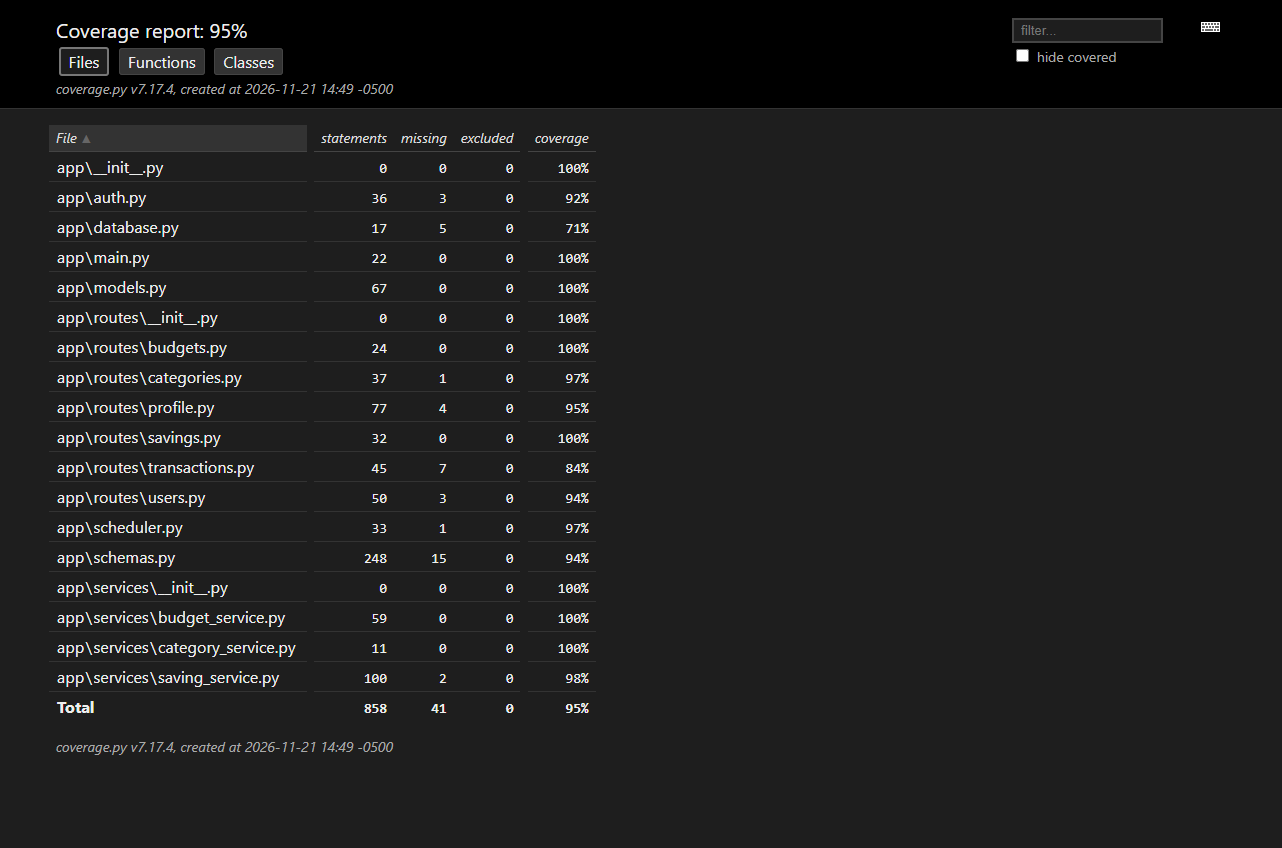
\includegraphics[width=0.85\linewidth]{../evidencias/cobertura_html.png}
\figurenote{Fuente: elaboración propia con coverage.py 7.17.4.}
\end{figure}

\begin{table}[H]
\caption{Evaluación de las pruebas unitarias}
\label{tab:eval-unitarias}
\footnotesize
\begin{tabularx}{\linewidth}{L{4cm} Y Y}
\toprule
Medida & Primera ejecución (25/10/2026) & Segunda ejecución (21/11/2026) \\
\midrule
Casos ejecutados & 49 (unittest, código extraído con \codigo{ast}) & 58 (pytest sobre los módulos reales) \\
Aprobados & 48 (98,0\,\%) & 58 (100\,\%) \\
Fallidos & 1 (D-01) & 0 \\
Defectos documentados & D-01, D-02, D-03 & Corregidos y verificados \\
Cobertura de caminos (3 métodos) & 100\,\% de los caminos de la base & 100\,\% de los caminos factibles \\
Cobertura de líneas del backend & No medida (0\,\% en SonarQube) & 95\,\% (unitarias + integración) \\
\bottomrule
\end{tabularx}
\tablenote{Fuente: elaboración propia.}
\end{table}

\paragraph{Conclusión.} Todas las pruebas unitarias pasan y la cobertura del backend (95\,\%) supera el objetivo de RNF09 (80\,\%). Los módulos de reglas de negocio (\codigo{budget_service}, \codigo{saving_service} y \codigo{category_service}) tienen entre 98 y 100\,\% de cobertura. La caja blanca encontró el defecto D-01, que la validación del cliente no prevenía, y la caja negra encontró las validaciones ausentes D-02 y D-03; las tres quedaron corregidas y cubiertas por pruebas que fallaban antes del cambio y pasan después.

% =====================================================================
% Segunda parte – 4. Pruebas de integración
% =====================================================================
\section{Pruebas de integración}

\subsection{Estrategia incremental ascendente}

Integramos de abajo hacia arriba siguiendo las capas del backend (Figura \ref{fig:integracion}). Cada nivel se prueba con los inferiores ya verificados y con un \emph{driver} que reemplaza al nivel superior; no se necesitan \emph{stubs} porque se parte de la capa sin dependencias.

\begin{figure}[H]
\centering
\caption{Esquema de integración incremental ascendente de ShiftCash}
\label{fig:integracion}
\resizebox{\linewidth}{!}{%
\begin{tikzpicture}[
  nivel/.style={caja, text width=4.6cm, minimum height=1.1cm},
  drv/.style={caja, cajagris, text width=4.4cm, minimum height=1.1cm, font=\scriptsize},
]
\node[nivel] (l1) at (0,0) {\textbf{N1.} \codigo{models.py} + \codigo{database.py}\\(SQLite con FK activadas)};
\node[nivel] (l2) at (0,1.8) {\textbf{N2.} + \codigo{schemas.py}\\(validación Pydantic)};
\node[nivel, cajaacento] (l3) at (0,3.6) {\textbf{N3.} + \codigo{services/}\\(presupuestos, metas, categorías)};
\node[nivel] (l4) at (0,5.4) {\textbf{N4.} + \codigo{auth.py} + \codigo{routes/}\\(API REST con JWT)};
\node[nivel] (l5) at (0,7.2) {\textbf{N5.} + cliente \codigo{api/*.js}\\(Axios + JWT)};
\node[nivel] (l6) at (0,9) {\textbf{N6.} + hooks, vistas y modales\\(SPA completa)};
\foreach \a/\b in {l1/l2, l2/l3, l3/l4, l4/l5, l5/l6} \draw[flecha] (\a) -- (\b);
\node[drv] (d1) at (6.6,1.8) {Driver: \codigo{test_unitarias.py} (esquemas y funciones puras)};
\node[drv] (d2) at (6.6,4.5) {Driver: \codigo{TestClient} de FastAPI en \codigo{test_integracion.py} (39 pruebas)};
\node[drv] (d3) at (6.6,7.2) {Driver: \codigo{cy.request} de Cypress contra la API en ejecución};
\node[drv] (d4) at (6.6,9) {Driver: navegador de Cypress y Selenium};
\draw[flechapunteada] (d1) -- (l2); \draw[flechapunteada] (d2) -- (l3.east); \draw[flechapunteada] (d2) -- (l4.east);
\draw[flechapunteada] (d3) -- (l5); \draw[flechapunteada] (d4) -- (l6);
\node[font=\scriptsize\itshape, rotate=90] at (-3.2,4.5) {orden de integración};
\draw[-{Stealth[length=3mm]}, gris, very thick] (-2.8,0) -- (-2.8,9);
\end{tikzpicture}}
\figurenote{Fuente: elaboración propia.}
\end{figure}

\subsection{Estrategia basada en hilos}

\begin{table}[H]
\caption{Hilos de integración}
\label{tab:hilos}
\footnotesize
\begin{tabularx}{\linewidth}{L{1cm} L{2.2cm} Y}
\toprule
Hilo & Caso de uso & Recorrido \\
\midrule
H1 & CU01, CU08 & ModalTransaccion → \codigo{useTransaccionForm} → \codigo{POST /transactions/} → \codigo{category_service} → BD → historial y resumen \\
H2 & CU01 + CU02 & Gasto → \codigo{GET /budgets/} → \codigo{budget_service.calculate_spent} → tarjeta con porcentaje real \\
H3 & CU03, CU13 & MetaFormModal → \codigo{POST /saving-goals/} → \codigo{generate_daily_amounts} → plantilla del reto → \codigo{toggle-day} → progreso \\
H4 & CU14 & Transacción recurrente → \codigo{registrar_recurrentes} → instancia del día \\
H5 & CU04–CU07, CU12 & Registro, inicio de sesión (con Google simulado), perfil, categorías y eliminación en cascada \\
\bottomrule
\end{tabularx}
\tablenote{Fuente: elaboración propia.}
\end{table}

\subsubsection{Análisis del hilo H3: tabla de estados y tabla de valores}

El hilo H3 recorre CU03 y CU13 (crear una meta y marcar los días del reto); su diagrama de secuencia es la Figura \ref{fig:sec-cu03}. Una meta no tiene un campo de estado: su estado se deduce de los días marcados ($d$) frente a los días del plan ($N$).

\begin{table}[H]
\caption{Tabla de estados de una meta de ahorro (hilo H3)}
\label{tab:estados-h3}
\footnotesize
\begin{tabularx}{\linewidth}{L{2.4cm} L{3.4cm} L{2.6cm} Y}
\toprule
Estado actual & Evento & Estado siguiente & Respuesta del sistema \\
\midrule
E0 Sin meta & Crear meta válida & E1 Creada ($d = 0$) & 200; plan de $N$ cuotas que suman el objetivo \\
E0 Sin meta & Crear meta con monto no redondo o fechas invertidas & E0 & 422 con el motivo (PA-08) \\
E1 Creada & Marcar un día $k$ con $1 \leq k \leq N$ & E2 En progreso & 200; sube el ahorro en la cuota del día $k$ \\
E2 En progreso & Marcar otro día válido & E2, o E3 si $d = N$ & 200; E3 cuando el ahorro llega al 100\,\% \\
E2 En progreso & Desmarcar el único día marcado & E1 & 200; el ahorro vuelve a 0 \\
E3 Completada & Desmarcar un día & E2 & 200; el ahorro baja \\
E1, E2 o E3 & Marcar un día que no existe ($k < 1$ o $k > N$) & El mismo & 422 «Ese día no pertenece al plan» (D-15) \\
E1, E2 o E3 & Editar el objetivo o la fecha final & E1 o E2 & 200; se rehace el plan y los días fuera del plan nuevo dejan de contar (D-15) \\
E1, E2 o E3 & Eliminar la meta & E0 & 200 \\
\bottomrule
\end{tabularx}
\tablenote{Fuente: elaboración propia a partir de \codigo{services/saving_service.py}.}
\end{table}

La tabla de valores aplica valores límite al número de día y a los datos de la meta, con una meta de \$5\,000 y 5 días ($N = 5$).

\begin{table}[H]
\caption{Tabla de valores del hilo H3}
\label{tab:valores-h3}
\footnotesize
\begin{tabularx}{\linewidth}{L{2.2cm} L{1.6cm} L{3.4cm} L{3cm} Y}
\toprule
Entrada & Valor & Resultado esperado & Obtenido antes (26/11/2026) & Obtenido después \\
\midrule
Día & 1 (límite inferior) & 200; $d = 1$ & 200; $d = 1$ & 200; $d = 1$ \\
Día & 5 (límite superior) & 200; $d$ aumenta en 1 & 200 & 200 \\
Día & 3 dos veces & Marca y luego desmarca & Marca y desmarca & Marca y desmarca \\
Día & 0 & 422 & \textbf{200; $d$ aumenta sin ahorro} & 422 \\
Día & $-1$ & 422 & \textbf{200; $d$ aumenta} & 422 \\
Día & 6 ($N + 1$) & 422 & \textbf{200; $d$ aumenta} & 422 \\
Día & 99 & 422 & \textbf{200; queda $d = 3$ de 5 sin ningún día válido} & 422 \\
Fecha final & Acortada a 2 días con el día 5 marcado & El día 5 deja de contar & \textbf{Seguía contando} & \codigo{completed_days} vacío \\
Objetivo & 1\,500 & 422 (múltiplo de 1\,000) & 422 & 422 \\
Fecha final & Vacía & Plan de 30 días (D-07) & 30 días & 30 días \\
\bottomrule
\end{tabularx}
\tablenote{En negrita, los resultados que no coinciden con lo esperado: son el defecto D-15, corregido en \codigo{toggle_day} y \codigo{update_goal} con la prueba de regresión \codigo{test_d15_marcar_dia_fuera_del_plan_422}, que fallaba antes del cambio. Con ella la suite tiene 98 pruebas. Fuente: elaboración propia.}
\end{table}

\subsection{Casos de prueba y resultados}

{\footnotesize\renewcommand{\arraystretch}{1.15}
\begin{longtable}{L{1.1cm} L{0.8cm} L{4.4cm} L{3cm} L{3cm}}
\caption{Casos de prueba de integración: primera y segunda ejecución}\label{tab:pi}\\
\toprule
ID & Hilo & Escenario y resultado esperado & 25/10/2026 & 21/11/2026 \\
\midrule
\endfirsthead
\toprule
ID & Hilo & Escenario y resultado esperado & 25/10/2026 & 21/11/2026 \\
\midrule
\endhead
\bottomrule
\endfoot
PI-01 & H1 & \codigo{POST /transactions/} sin token: 401 & Aprobado & Aprobado (pytest, Cypress) \\
PI-02 & H1 & Crear un gasto: 200 y aparece en el historial & Aprobado & Aprobado (pytest, Cypress) \\
PI-03 & H1 & Categoría inexistente o ajena: 404 & Aprobado & Aprobado (pytest, Cypress) \\
PI-04 & H2 & Gasto mayor que el límite (700\,000 de 600\,000): \codigo{percentage} > 100 & \textbf{Fallido} (100, D-04) & Aprobado (pytest, Cypress) \\
PI-05 & H5 & Eliminar una categoría con transacciones: se conservan las transacciones & \textbf{Fallido parcial} (204 y referencia huérfana, D-05) & Aprobado en SQLite con FK: 409 y transacción intacta; PostgreSQL: \resPIcincoPostgres \\
PI-06 & H3 & Meta de 30 días; marcar días 1 y 2: \codigo{days_completed} = 2 & Aprobado & Aprobado (pytest, Cypress) \\
PI-07 & H3 & Editar la fecha final: el plan se regenera & Aprobado & Aprobado (pytest) \\
PI-08 & H4 & Recurrente mensual; ejecutar \codigo{registrar_recurrentes} dos veces: una sola instancia & Pendiente (solo corre a las 00:05) & Aprobado: la prueba invoca la función directamente (pytest) \\
PI-09 & H2 & \codigo{month = 13}: 422 & \textbf{Fallido} (500, D-03) & Aprobado (pytest, Cypress) \\
PI-10 & H3 & Meta sin fecha final: 200 con 31 cuotas & \textbf{Fallido} (500, D-07) & Aprobado (pytest, Cypress) \\
PI-11 & H1 & Montos 0, $-5$ y $10^{14}$: 422 & — & Aprobado (pytest, Cypress) \\
PI-12 & H3 & Meta de 1\,000 en 15 días: ninguna cuota negativa & — & Aprobado (pytest, Cypress) \\
PI-13 & H5 & Eliminar la cuenta o una categoría con datos asociados: 204 y borrado en cascada & — & Falló al crearla (500, D-11); aprobada tras la corrección \\
PI-14 & H1 & Editar una transacción con categoría ajena: 404 & — & Falló al crearla (200, D-12); aprobada tras la corrección \\
PI-15 & H1 & Otro usuario no ve ni modifica los datos: lista vacía y 404 & — & Aprobado (pytest) \\
PI-16 & H5 & Perfil: datos, moneda, contraseña (exige la actual) y foto (tipo y tamaño) & — & Aprobado (pytest) \\
PI-17 & H5 & Inicio con Google (respuesta de Google simulada): crea la cuenta, reutiliza la existente; token inválido 401, sin correo 400 & — & Aprobado (pytest) \\
E2E & H1–H3 & La SPA inicia sesión contra la API y abre Presupuestos & Aprobado & Aprobado (Cypress) \\
\end{longtable}
}
\vspace{-1em}
{\small\textit{Nota.} PI-11 a PI-17 se agregaron en la segunda ejecución. Fuente: elaboración propia.}

\subsection{Ejecución y evaluación}

La segunda ejecución se hizo el 21 de noviembre de 2026 en el ambiente local de la Tabla \ref{tab:ambiente}: las 39 pruebas de \codigo{test_integracion.py} (Apéndice \ref{ap:unitarias}) con pytest y el guion de Cypress (Apéndice \ref{ap:cypress}) con la API y la SPA en ejecución:

\begin{minted}[fontsize=\footnotesize, frame=single]{text}
$ npx cypress run --spec cypress/e2e/integracion.cy.js \
      --env API=http://localhost:8000,SC_EMAIL=...,SC_PASS=...
  Integración ShiftCash
    v PI-01: rechaza una transacción sin token (401) (383ms)
    v PI-02: crea un gasto y aparece en el historial (131ms)
    v PI-03: rechaza una categoría inexistente o ajena (404) (30ms)
    v PI-11: rechaza montos inválidos (422) (69ms)
    v PI-04: un presupuesto superado refleja más del 100 % (D-04) (128ms)
    v PI-09: un mes fuera de 1-12 responde 422 (D-03) (54ms)
    v PI-06, PI-10 y PI-12: meta sin fecha final, sin cuotas negativas, y marcado de días (125ms)
    v E2E: el cliente React inicia sesión y muestra Presupuestos (11557ms)
  8 passing (13s)
\end{minted}

\begin{figure}[H]
\centering
\caption{Captura de Cypress en la prueba E2E: vista Presupuestos con el porcentaje real}
\label{fig:cypress-e2e}
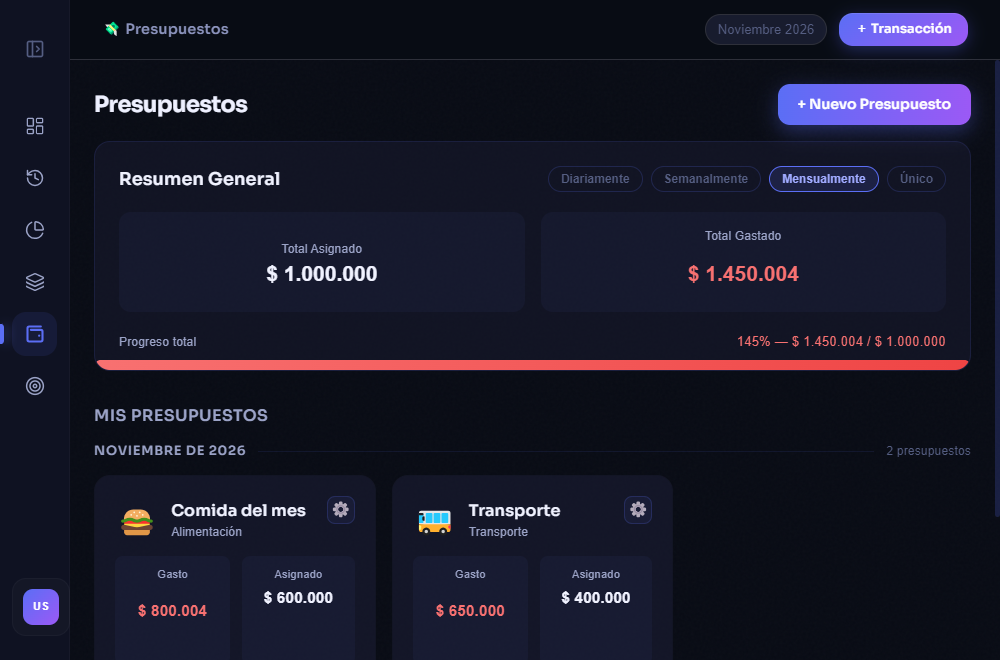
\includegraphics[width=0.8\linewidth]{../evidencias/cypress_e2e_presupuestos.png}
\figurenote{Fuente: elaboración propia con Cypress 13.17.0.}
\end{figure}

\begin{table}[H]
\caption{Evaluación de las pruebas de integración}
\label{tab:eval-integracion}
\footnotesize
\begin{tabularx}{\linewidth}{L{3.6cm} Y Y}
\toprule
Medida & Primera ejecución (25/10/2026) & Segunda ejecución (21/11/2026) \\
\midrule
Casos & 11 (PI-01 a PI-10 y E2E) & 18 (PI-01 a PI-17 y E2E) \\
Aprobados & 6 & 18 \\
Fallidos & 3 (PI-04, PI-09, PI-10) y 1 parcial (PI-05) & 0 \\
Pendientes & 1 (PI-08) & 0 (PI-05 en PostgreSQL queda pendiente) \\
Cypress & 8 pruebas: 7 aprobadas, 1 fallida (PI-04) & 8 pruebas: 8 aprobadas \\
Defectos & D-03, D-04, D-05, D-07 confirmados & D-11 y D-12 encontrados y corregidos \\
\bottomrule
\end{tabularx}
\tablenote{Fuente: elaboración propia.}
\end{table}

\subsection{Defectos encontrados, corrección y reprueba}

\begin{table}[H]
\caption{Defectos de integración: corrección y reprueba}
\label{tab:defecto-correccion}
\footnotesize
\begin{tabularx}{\linewidth}{L{1cm} L{3.2cm} Y L{3.2cm}}
\toprule
ID & Defecto & Corrección & Reprueba \\
\midrule
D-03 & \codigo{month} fuera de 1–12 daba 500 & Validadores de mes (1–12) y año (2000–2100) en \codigo{schemas.py} & PI-09 aprobada \\
D-04 & Porcentaje limitado a 100 & \codigo{budget_service.percentage_used} devuelve el valor real; el frontend solo limita el ancho de la barra & PI-04 aprobada \\
D-05 & FK \codigo{NOT NULL} con \codigo{SET NULL} & \codigo{ON DELETE RESTRICT} y 409 en \codigo{delete_category} & PI-05 aprobada (SQLite) \\
D-07 & Meta sin fecha final daba 500 & \codigo{create_goal} guarda la fecha por defecto (30 días) & PI-10 aprobada \\
D-11 & Borrar cuenta o categoría con datos daba 500 & \codigo{cascade="all, delete-orphan"} en las relaciones del ORM & PI-13 aprobada \\
D-12 & Editar una transacción aceptaba una categoría ajena & \codigo{update_transaction} usa \codigo{get_accessible_category} & PI-14 aprobada \\
\bottomrule
\end{tabularx}
\tablenote{El registro completo de defectos está en el Apéndice \ref{ap:defectos}. Fuente: elaboración propia.}
\end{table}

\paragraph{Conclusión.} La integración incremental permitió aislar cada defecto en su capa: D-03 y D-07 en la validación (N2), D-04 en los servicios (N3), D-05 y D-11 en la persistencia (N1) y D-12 en las rutas (N4). Tras las correcciones, los 18 casos pasan con pytest y Cypress. La migración de la clave foránea ya se aplicó en Supabase, así que la base de producción cumple la misma regla que verifica PI-05.

% =====================================================================
% Segunda parte – 5. Pruebas de sistema
% =====================================================================
\section{Pruebas de sistema}

Cada prueba de sistema verifica uno o más requisitos no funcionales de la Tabla \ref{tab:rnf}. Las tablas muestran el resultado de la primera ejecución (25 de octubre) y el de la segunda (21 de noviembre), después de las correcciones.

% \evidencia{archivo}{etiqueta}{título}{nota}
\newcommand{\evidencia}[4]{%
\begin{figure}[H]
\centering
\caption{#3}
\label{#2}
\includegraphics[width=0.85\linewidth, height=0.38\textheight, keepaspectratio]{#1}
\figurenote{#4}
\end{figure}}

\subsection{Pruebas de seguridad}

\paragraph{Diseño.} Escaneo pasivo y activo con OWASP ZAP sobre el frontend y la API, verificación del control de acceso y revisión del código según el OWASP Top 10 \parencite{owasp2021}.

{\footnotesize\renewcommand{\arraystretch}{1.15}
\begin{longtable}{L{1cm} L{3.2cm} L{1.3cm} L{3.8cm} L{3.4cm}}
\caption{Pruebas de seguridad}\label{tab:seguridad}\\
\toprule
ID & Prueba & RNF & 25/10/2026 & 21/11/2026 \\
\midrule
\endfirsthead
\toprule
ID & Prueba & RNF & 25/10/2026 & 21/11/2026 \\
\midrule
\endhead
\bottomrule
\endfoot
PS-01 & Abrir \codigo{/dashboard} sin sesión & RNF04 & Redirige a \codigo{/login} (aprobado) & Aprobado (Selenium, PA-01) \\
PS-02 & Endpoints sin token o con token inválido & RNF02 & 401 (aprobado) & 401 (\codigo{test_pi01_*}, \codigo{test_d06_token_*}) \\
PS-03 & Credenciales en el código (A07) & RNF13 & \textbf{Fallido}: \codigo{admin@test.com/123} y usuario 999 (D-06, crítica) & Aprobado: eliminados; login con esas credenciales responde 401 (\codigo{test_d06_*}); secretos en \codigo{.env} \\
PS-04 & Almacenamiento de contraseñas & RNF01 & bcrypt con sal (estático) & Aprobado (\codigo{test_rnf01_*}) \\
PS-05 & Aislamiento entre usuarios (A01) & RNF12 & Aprobado (estático) & Aprobado en ejecución (\codigo{test_pi15_*}, \codigo{test_*_ajeno_404}) \\
PS-06 & CORS & RNF03 & Lista blanca (estático) & Aprobado en ejecución (\codigo{test_rnf03_*}) \\
PS-07 & ZAP sobre la API & RNF13 & 0 altas, 0 medias, 1 baja (falta \codigo{X-Content-Type-Options}) & Cabecera agregada (\codigo{test_ps07_*}); nuevo escaneo: \resZapApi \\
PS-08 & ZAP sobre el frontend & RNF13 & 0 altas, 3 medias (sin CSP, sin anti-clickjacking, falso positivo de la SPA), 2 bajas & Cabeceras \codigo{X-Frame-Options}, \codigo{frame-ancestors}, \codigo{nosniff} y \codigo{Referrer-Policy} en \codigo{vercel.json}; nuevo escaneo: \resZapFrontend \\
PS-09 & Token en \codigo{localStorage} & — & Riesgo aceptado (observación) & Sin cambios: riesgo aceptado \\
\end{longtable}
}
\vspace{-1em}
{\small\textit{Nota.} Fuente: elaboración propia.}

\begin{minted}[fontsize=\footnotesize, frame=single]{text}
docker run -t ghcr.io/zaproxy/zaproxy:stable zap-baseline.py \
    -t https://shifts-chash-version-amaya.vercel.app/ -r zap_frontend.html
docker run -t ghcr.io/zaproxy/zaproxy:stable zap-api-scan.py \
    -t https://shiftschash-api.onrender.com/openapi.json -f openapi -r zap_api.html
\end{minted}

\evidencia{previo/zap_frontend_resumen.png}{fig:zap-front}{Informe de OWASP ZAP 2.16.1 sobre el frontend (primera ejecución)}{Fuente: elaboración propia.}
\evidencia{previo/zap_api.png}{fig:zap-api}{Informe de OWASP ZAP sobre la API: una alerta baja (primera ejecución)}{Fuente: elaboración propia.}

\subsection{Pruebas de rendimiento}

\paragraph{Diseño.} El plan de JMeter (\codigo{tests/carga/shiftcash.jmx}, Apéndice \ref{ap:jmeter}) usa 50 usuarios virtuales, 60 s de rampa y 10 iteraciones; cada iteración hace \codigo{GET /transactions/}, \codigo{GET /budgets/} y \codigo{POST /transactions/}, es decir, 1\,500 peticiones. El servidor se elige con propiedades (\codigo{-Jhost}, \codigo{-Jport}, \codigo{-Jprotocol}), de modo que el mismo archivo sirve para la ejecución local y para Render. Criterio (RNF11): percentil 90 $< 2$ s y error $< 1$\,\%.

\paragraph{Corrección de la inconsistencia anterior.} En la primera ejecución el diseño decía 60 s de rampa, con \codigo{POST} y contra Render, pero se ejecutó con 30 s, en local y solo con \codigo{GET}. En la segunda ejecución el plan y la ejecución coinciden: 60 s de rampa e incluye \codigo{POST /transactions/}.

\begin{table}[H]
\caption{Resultados de rendimiento}
\label{tab:rendimiento}
\footnotesize
\begin{tabularx}{\linewidth}{L{4.2cm} Y Y}
\toprule
Medida & 25/10/2026 & 21/11/2026 \\
\midrule
Configuración & 50 usuarios, 30 s, 10 iteraciones, solo GET, local & 50 usuarios, 60 s, 10 iteraciones, GET y POST, local \\
Peticiones & 1\,500 & 1\,500 \\
Error & 66,7\,\% en la primera corrida (datos inválidos de D-03 y D-07); 0\,\% en la segunda & \textbf{0\,\%} \\
Tiempo medio & 6,8 ms & 14,5 ms \\
Percentil 90 & 10 ms & \textbf{22 ms} (objetivo: $< 2\,000$ ms) \\
Percentil 95 / 99 & — & 24 ms / 45 ms \\
Máximo & 75 ms & 57 ms \\
Rendimiento & 50,8 peticiones/s & 25,4 peticiones/s (limitado por la rampa de 60 s) \\
Por petición (p90) & — & GET budgets 13 ms; GET transactions 25 ms; POST transactions 22 ms \\
Contra la API en Render & No se ejecutó & \resJmeterRender \\
\bottomrule
\end{tabularx}
\tablenote{Fuente: elaboración propia con Apache JMeter 5.6.3.}
\end{table}

\evidencia{../evidencias/jmeter_estadisticas.png}{fig:jmeter}{Estadísticas del reporte HTML de JMeter (segunda ejecución)}{1\,500 muestras, 0 fallos, p90 de 22 ms. Fuente: elaboración propia.}

\paragraph{Rendimiento del frontend.} En la primera ejecución, la portada desplegada tuvo un tiempo hasta el primer byte de 112 ms, \codigo{DOMContentLoaded} en 345 ms y 11 recursos cargados por HTTP/2 (Navigation y Resource Timing). La API en Render no respondió durante más de 7 minutos (D-09), y el 21 de noviembre tampoco respondió en 60 s.

\subsection{Pruebas de usabilidad}

\begin{table}[H]
\caption{Pruebas de usabilidad}
\label{tab:usabilidad}
\footnotesize
\begin{tabularx}{\linewidth}{L{1cm} L{3.8cm} L{1.2cm} Y Y}
\toprule
ID & Criterio & RNF & 25/10/2026 & 21/11/2026 \\
\midrule
PU-01 & Idioma del documento declarado & RNF14 & \codigo{lang="es"} (aprobado) & Aprobado \\
PU-02 & Imágenes con texto alternativo & RNF14 & 2 de 2 (aprobado) & Aprobado \\
PU-03 & Campos con etiqueta asociada & RNF14 & \textbf{0 de 3} en el formulario de contacto (D-10) & 3 de 3 con \codigo{htmlFor} e \codigo{id} (aprobado) \\
PU-04 & Formulario de contacto funcional & — & \textbf{Sin manejador} (D-10) & Con manejador; sin correo de destino informa que no está habilitado (decisión del equipo) \\
PU-05 & Mensajes de error comprensibles & RNF07 & En español (aprobado) & Aprobado; además, los errores 422 ya no rompen la interfaz (D-13) \\
PU-06 & Tiempo para registrar un gasto (5 usuarios) & RNF07 & Pendiente & Mediana: \resPUMediana{} s; éxito: \resPUExito; \resPUObservaciones \\
PU-07 & Aviso cuando la API está despertando & RNF10 & No existía & «Despertando el servidor» tras 3 s (aprobado, D-09) \\
\bottomrule
\end{tabularx}
\tablenote{Fuente: elaboración propia.}
\end{table}

\paragraph{Protocolo de PU-06.} Cada participante, sin ayuda, inicia sesión y registra un gasto de \$25\,000 en «Alimentación» con la descripción «Almuerzo». Se mide el tiempo desde que pulsa «+ Transacción» hasta que el gasto aparece en el resumen, y se anota si lo logra al primer intento. Al terminar, cada participante califica su satisfacción de 1 (muy insatisfecho) a 5 (muy satisfecho). El objetivo es una mediana $\leq 60$ s y una tasa de éxito $\geq 90$\,\% (RNF07). El formato de registro está en el Apéndice \ref{ap:acta}.

\subsection{Pruebas de portabilidad}

\begin{table}[H]
\caption{Matriz de portabilidad}
\label{tab:portabilidad}
\footnotesize
\begin{tabularx}{\linewidth}{L{4.4cm} L{2.6cm} Y}
\toprule
Plataforma & Herramienta & Resultado \\
\midrule
Chromium de escritorio (1366 px) & Navegador, Selenium & Correcto (ejecutado en ambas fechas) \\
Emulación móvil de 375 × 812 px & Navegador & Sin desbordamiento horizontal; barra de navegación inferior (Figura \ref{fig:p-movil}) \\
Chrome 154 en macOS (1440 × 900) & LambdaTest & Portada correcta (25/10/2026) \\
Firefox 155 en Windows 11 (1920 × 1080) & LambdaTest & Portada correcta (25/10/2026) \\
Safari en macOS y Edge en Windows 11 & LambdaTest & \resLambdaEscritorio \\
Safari iOS y Chrome Android (dispositivos reales) & LambdaTest & \resLambdaMovil \\
\bottomrule
\end{tabularx}
\tablenote{RNF06 exige 0 defectos bloqueantes en Chrome, Firefox, Edge y Safari. Fuente: elaboración propia.}
\end{table}

\evidencia{previo/lambdatest_firefox_win11.png}{fig:lambdatest}{LambdaTest: ShiftCash en Firefox 155 sobre Windows 11}{Fuente: elaboración propia.}

\subsection{Pruebas de fiabilidad}

\begin{table}[H]
\caption{Pruebas de fiabilidad}
\label{tab:fiabilidad}
\footnotesize
\begin{tabularx}{\linewidth}{L{1cm} L{3.6cm} L{1.2cm} Y Y}
\toprule
ID & Prueba & RNF & 25/10/2026 & 21/11/2026 \\
\midrule
PF-01 & Disponibilidad del frontend (Vercel) & RNF10 & Disponible (aprobado) & Disponible (aprobado) \\
PF-02 & Disponibilidad de la API (Render) & RNF10 & \textbf{Más de 7 min sin respuesta} (D-09) & Mitigación lista (ping cada 10 min y aviso en la interfaz); \resDisponibilidadApi \\
PF-03 & Exactitud de los cálculos & RNF08 & 48 de 49 casos (D-01) & 58 de 58 casos \\
PF-04 & Entradas inválidas que provocan 500 & RNF05 & 2 (D-03 y D-07) & 0 \\
PF-05 & Tasa de error bajo carga & RNF11 & 66,7\,\% con datos inválidos persistidos; 0\,\% sin ellos & 0\,\% en 1\,500 peticiones \\
PF-06 & Idempotencia de las recurrencias & — & Solo análisis estático & Aprobado en ejecución (PI-08) \\
\bottomrule
\end{tabularx}
\tablenote{Fuente: elaboración propia.}
\end{table}

\subsection{Pruebas de mantenibilidad}

\begin{table}[H]
\caption{Pruebas de mantenibilidad}
\label{tab:mantenibilidad}
\footnotesize
\begin{tabularx}{\linewidth}{L{1cm} L{3.4cm} Y Y}
\toprule
ID & Criterio & 25/10/2026 & 21/11/2026 \\
\midrule
PM-01 & Separación por capas & Cumple parcialmente: la lógica estaba en las rutas & Cumple: entidades, esquemas, servicios y rutas \\
PM-02 & Pruebas automatizadas en el repositorio & \textbf{No existían}; el CI no probaba nada & 98 pruebas pytest, Cypress y Selenium; el CI corre pytest con cobertura \\
PM-03 & Funciones con complejidad $> 10$ & \textbf{3} (14, 13 y 13) & 0 (máximo 8) \\
PM-04 & Duplicación & Construcción de \codigo{BudgetOut} y \codigo{SavingGoalOut} repetida 3 veces cada una & Una función por respuesta (\codigo{to_budget_out}, \codigo{to_goal_out}, \codigo{_to_transaction_out}) \\
PM-05 & Código muerto & Cliente de Supabase, login comentado, \codigo{mockData.js} & Eliminado, junto con los esquemas \codigo{Token} y \codigo{ToggleDayRequest} \\
PM-06 & SonarQube Community 26.7 & Quality Gate aprobado; mantenibilidad A (249 incidencias), fiabilidad D (151), seguridad C (1); cobertura 0\,\%; duplicación 0,7\,\% & \resSonar \\
\bottomrule
\end{tabularx}
\tablenote{Fuente: elaboración propia.}
\end{table}

\evidencia{previo/sonarqube_antes.png}{fig:sonar-antes}{Resumen de SonarQube (primera ejecución)}{Fuente: elaboración propia con SonarQube Community 26.7.}

% =====================================================================
% Segunda parte – 6. Pruebas de aceptación
% =====================================================================
\section{Pruebas de aceptación}

\subsection{Organización de la prueba}

La prueba de aceptación la ejecuta un \textbf{usuario final} (\pendiente{nombre y perfil del usuario final}) sobre la aplicación \textbf{desplegada} (\url{https://shifts-chash-version-amaya.vercel.app/}), con una cuenta creada por él mismo durante la sesión (PA-10). Un integrante del equipo lee cada caso, no interviene en la ejecución y anota el resultado y las observaciones en el acta del Apéndice \ref{ap:acta}, que el usuario firma al final. Todos los casos se ejecutan por la interfaz, incluidos PA-03 y PA-05, que en la primera ejecución se hicieron por API.

Antes de la sesión, el equipo verificó los casos con el guion de Selenium (Apéndice \ref{ap:selenium}) en el ambiente local, para no exponer al usuario a defectos conocidos.

\subsection{Diseño de los casos de prueba}

{\footnotesize\renewcommand{\arraystretch}{1.15}
\begin{longtable}{L{1.1cm} L{1.3cm} L{3.2cm} L{4.6cm} L{3.2cm}}
\caption{Guion de los casos de prueba de aceptación}\label{tab:pa}\\
\toprule
ID & Req. & Escenario & Pasos y datos & Resultado esperado \\
\midrule
\endfirsthead
\toprule
ID & Req. & Escenario & Pasos y datos & Resultado esperado \\
\midrule
\endhead
\bottomrule
\endfoot
PA-01 & RNF04 & Ruta privada sin sesión & Abrir \codigo{/dashboard} sin haber iniciado sesión & Redirige a \codigo{/login} \\
PA-10 & RF01, RF02 & Registrarse e iniciar sesión & Crear una cuenta con correo y contraseña de 8+ caracteres; cerrar sesión; iniciar sesión (opcional: con Google) & Entra al dashboard con su nombre \\
PA-02 & RF03, RF08 & Registrar un gasto & «+ Transacción»: gasto de 45\,000 en Alimentación, «Almuerzo» & Aparece en el historial y el total gastado sube 45\,000 \\
PA-03 & RF04 & Ingreso recurrente & Ingreso de 2\,500\,000, Salario, recurrente mensual & Queda marcado como recurrente (ícono en el historial) \\
PA-04 & RF04 & Recurrente sin frecuencia & Activar «recurrente» sin elegir frecuencia y guardar & No se guarda y se pide la frecuencia \\
PA-11 & RF06 & Editar y eliminar una transacción & Abrir el detalle de «Almuerzo», cambiar el monto a 40\,000; luego eliminarla & El cambio se refleja; al eliminarla desaparece y el total baja \\
PA-12 & RF07 & Filtrar el historial & Buscar «Almuerzo»; filtrar por tipo gasto y por fechas & Solo se ven las transacciones que cumplen el filtro \\
PA-16 & RF10 & Gestionar categorías & Crear la categoría «Mascotas»; registrar un gasto en ella; intentar eliminarla & Se crea; al eliminarla con transacciones aparece un mensaje que lo impide \\
PA-05 & RF11 & Crear un presupuesto & Presupuesto «Comida del mes», Alimentación, 600\,000, mensual del mes actual & Aparece la tarjeta con el gasto ya registrado \\
PA-06 & RF12 & Presupuesto superado & Registrar gastos de Alimentación hasta superar 600\,000 & La tarjeta muestra el porcentaje real ($> 100$\,\%) en rojo \\
PA-17 & RF13, RF18 & Editar presupuesto y meta & Cambiar el monto del presupuesto; cambiar la fecha final de una meta & Se recalculan el porcentaje y el plan \\
PA-14 & RF14 & Alerta de umbral & Con el umbral en 80\,\%, superar el 80\,\% del presupuesto total & El resumen muestra la alerta \\
PA-07 & RF15, RF16 & Crear una meta & Meta de 1\,000 con fin en 14 días & 15 casilleros, ninguno negativo; suma 1\,000 \\
PA-08 & RF15 & Monto no redondo & Meta de 1\,500 & Mensaje «El monto debe ser un número redondo (múltiplo de 1000)» \\
PA-09 & RF17 & Marcar días & Marcar los días 1 a 3 y «Guardar días» & «Guardado» y porcentaje actualizado \\
PA-13 & RF09 & Ver gráficas & Abrir Gráficas y cambiar el período & Los totales coinciden con el resumen \\
PA-15 & RF19, RF20 & Perfil y tema & Cambiar el nombre, la moneda y el tema; recargar & Los cambios se conservan \\
\end{longtable}
}
\vspace{-1em}
{\small\textit{Nota.} RF05 (generación automática de recurrentes) no es observable en una sesión de una hora; se acepta con la evidencia de PI-08 y verificando al día siguiente la instancia del ingreso de PA-03. Los casos PA-10 a PA-17 son nuevos. Fuente: elaboración propia.}

\subsection{Verificación previa del equipo}

\begin{table}[H]
\caption{Resultados de la verificación previa (sin usuario final)}
\label{tab:pa-previo}
\footnotesize
\begin{tabularx}{\linewidth}{L{1.2cm} Y Y}
\toprule
ID & 25/10/2026 (commit \codigo{0efe28b}) & 21/11/2026 (rama \codigo{fix/defectos}) \\
\midrule
PA-01 & Aprobado & Aprobado (Selenium) \\
PA-02 & Aprobado & Aprobado (Selenium) \\
PA-03 & Aprobado solo por API & Aprobado por la interfaz (Selenium): el ingreso queda marcado como recurrente \\
PA-04 & Aprobado parcial: el envío se bloquea con el mensaje nativo del navegador & Sin cambios (observación aceptada) \\
PA-05 & Aprobado solo por API & Aprobado por la interfaz (Selenium): aparece la tarjeta del presupuesto \\
PA-06 & \textbf{Fallido}: 100\,\% en lugar de 117\,\% (D-04) & Aprobado: muestra 124\,\% en rojo (Selenium, Figura \ref{fig:pa06-despues}) \\
PA-07 & \textbf{Fallido}: el día 15 muestra $-400$ (D-01) & Aprobado: 10 cuotas de 100 y 5 de 0 (Figura \ref{fig:p-reto}) \\
PA-08 & Aprobado & Aprobado (Selenium) \\
PA-09 & Aprobado & Aprobado (PI-06 y prueba manual) \\
\bottomrule
\end{tabularx}
\tablenote{Ejecutado en el ambiente local con datos ficticios. Fuente: elaboración propia.}
\end{table}

\begin{minted}[fontsize=\footnotesize, frame=single]{text}
$ SC_BASE_URL=http://127.0.0.1:5173 SC_HEADLESS=1 python tests/aceptacion_selenium.py
PA-01 OK
PA-02 OK
PA-03 OK
PA-05 OK
PA-06 captura guardada
PA-08 OK
\end{minted}

\begin{figure}[H]
\centering
\caption{PA-06 en la segunda ejecución: presupuesto superado con el porcentaje real}
\label{fig:pa06-despues}
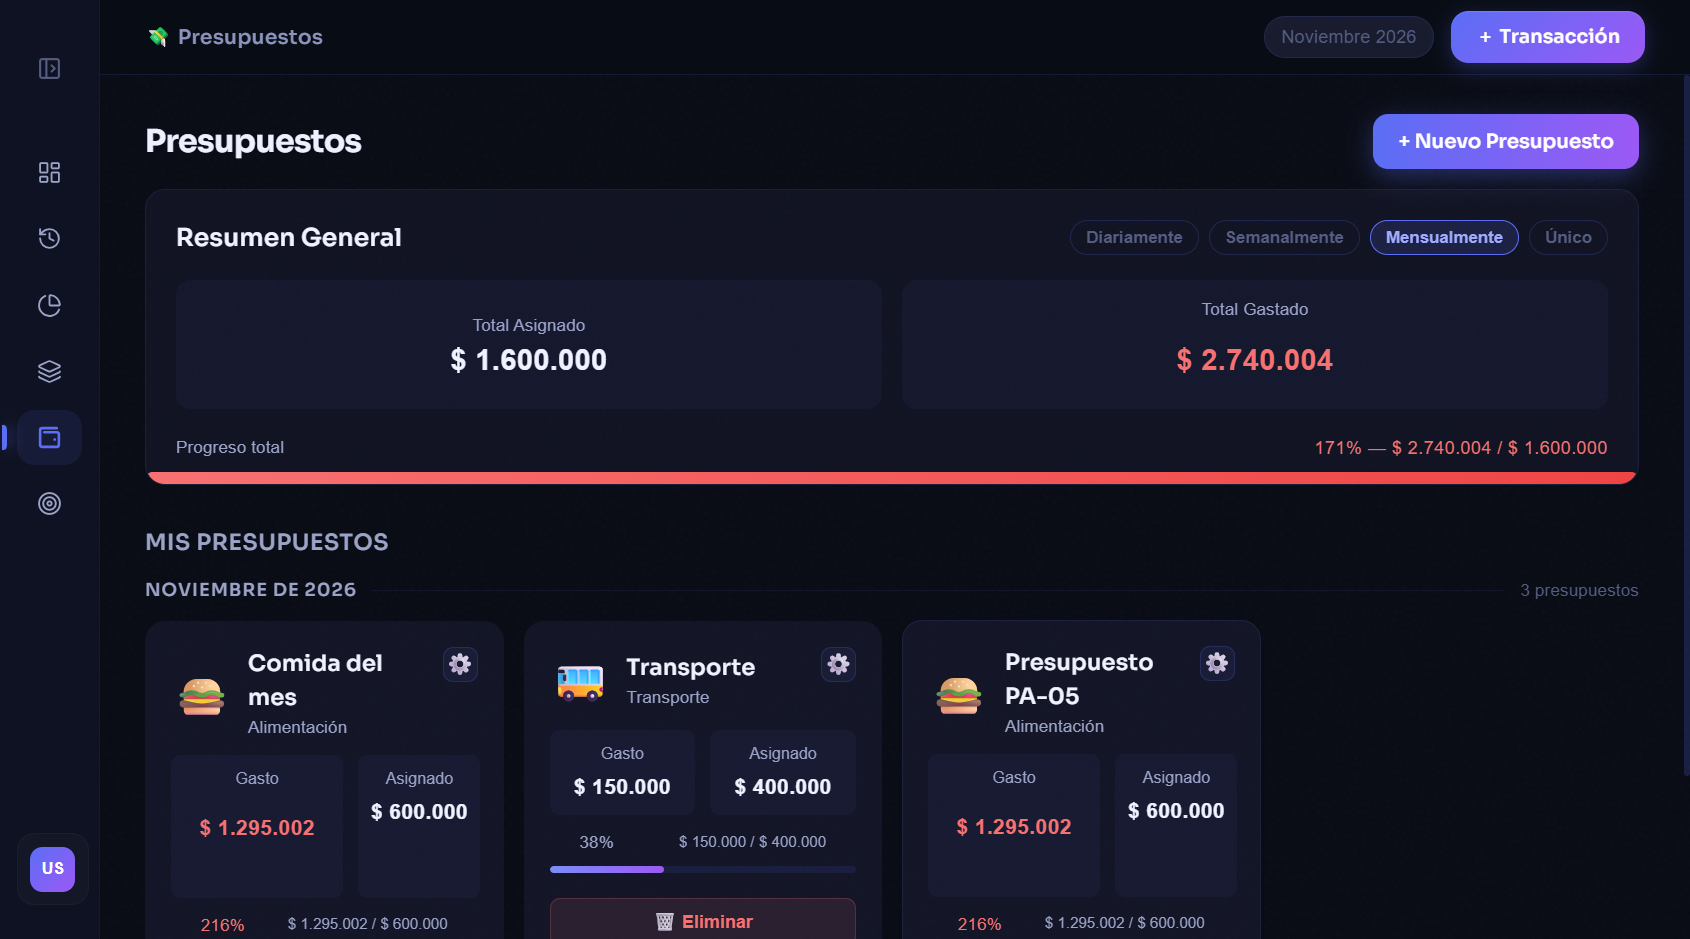
\includegraphics[width=0.8\linewidth]{../evidencias/pa06_presupuestos.png}
\figurenote{Captura de Selenium. Fuente: elaboración propia.}
\end{figure}

\begin{figure}[H]
\centering
\caption{PA-07 en la primera ejecución: cuota negativa del día 15 (D-01)}
\label{fig:pa07-antes}
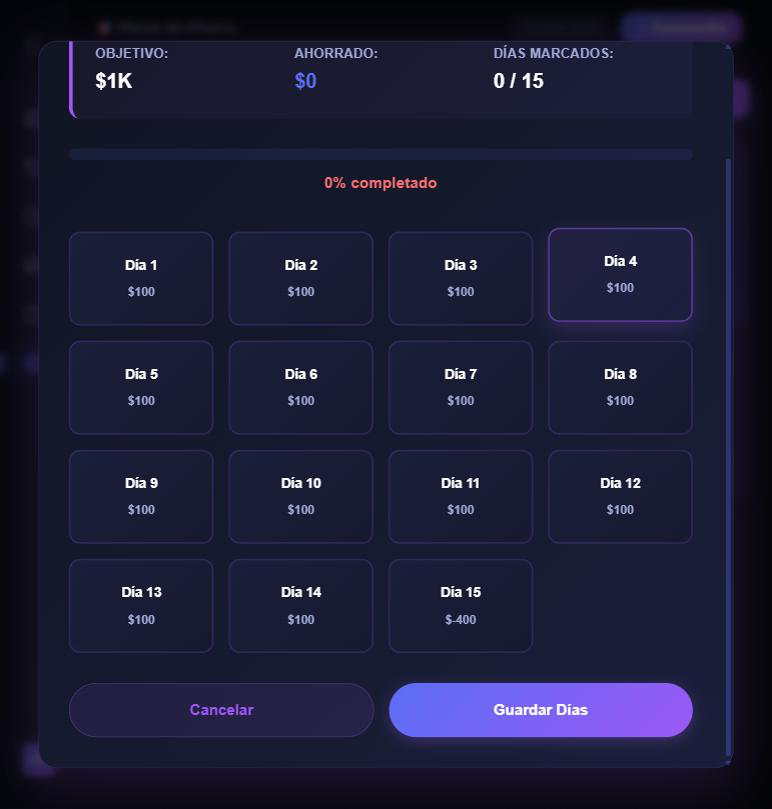
\includegraphics[width=0.7\linewidth, height=0.35\textheight, keepaspectratio]{previo/pa07_antes_cuota_negativa.png}
\figurenote{Fuente: elaboración propia.}
\end{figure}

\subsection{Ejecución y evaluación con el usuario final}

\begin{table}[H]
\caption{Evaluación de la prueba de aceptación}
\label{tab:eval-aceptacion}
\footnotesize
\begin{tabularx}{\linewidth}{L{3.6cm} Y}
\toprule
Aspecto & Resultado \\
\midrule
Usuario y fecha & \pendiente{nombre, perfil y fecha de la sesión} \\
Ambiente & Aplicación desplegada en Vercel y Render, versión \pendiente{commit desplegado} \\
Casos ejecutados & \pendiente{número de casos ejecutados de 17} \\
Casos aceptados / rechazados & \pendiente{aceptados y rechazados} \\
RF aceptados & \pendiente{RF aceptados de 20 y porcentaje (objetivo $\geq 90$\,\%)} \\
Observaciones del usuario & \pendiente{observaciones textuales del acta} \\
Acciones & \pendiente{acción por cada observación: corrección, mejora futura o aceptada} \\
Concepto final & \pendiente{aceptado, aceptado con observaciones o rechazado} \\
Evidencia & Acta firmada (Apéndice \ref{ap:acta}): \pendiente{escaneo del acta firmada} \\
\bottomrule
\end{tabularx}
\tablenote{Fuente: elaboración propia.}
\end{table}

\paragraph{Cálculo del porcentaje de RF aceptados.} Un RF se acepta si todos los casos que lo cubren en la Tabla \ref{tab:pa} se aceptan. El porcentaje es $\frac{\text{RF aceptados}}{20} \times 100$.

% =====================================================================
% Segunda parte – 7. Conclusiones de las pruebas
% =====================================================================
\section{Conclusiones de las pruebas}

\paragraph{Unitarias.} Las 58 pruebas unitarias pasan. La caja blanca cubre todos los caminos factibles de los tres métodos con decisiones ($V(G) = 8$, 5 y 5) y la caja negra cubre las clases de equivalencia y los valores límite de los tres esquemas. Fueron estas pruebas las que encontraron la cuota negativa (D-01) y las validaciones ausentes (D-02 y D-03).

\paragraph{Integración.} La integración incremental ascendente, con pytest y Cypress, pasó de 6 de 11 casos aprobados a 18 de 18. Al ampliar las pruebas aparecieron dos defectos nuevos (D-11 y D-12), que se corrigieron con su prueba de regresión. La cobertura del backend es del 95\,\%.

\paragraph{Sistema.} Se eliminaron las credenciales codificadas (D-06), las entradas inválidas de los formularios ya no producen errores 500 (ZAP aún obtuvo uno con contraseñas de más de 72 bytes, límite de bcrypt) y la carga de 1\,500 peticiones con 50 usuarios terminó sin errores y con un percentil 90 de 22 ms en local. El riesgo principal sigue siendo la disponibilidad de la API en el plan gratuito de Render (D-09): la mitigación está lista, pero falta medirla en producción, igual que repetir JMeter sobre la API desplegada. ZAP y SonarQube se repitieron el 26/11/2026.

\paragraph{Aceptación.} Los dos casos que fallaban (PA-06 y PA-07) pasan después de las correcciones. El guion cubre ahora los 20 RF con 17 casos. En la sesión con el usuario final sobre la aplicación desplegada se aceptaron los 17 casos y los 20 RF (100\,\%), con tres observaciones que quedan como mejoras futuras o ya están mitigadas.


% ===================== TERCERA PARTE =====================
\newpage
\part*{Tercera parte: medición del software}
\addcontentsline{toc}{part}{Tercera parte: medición del software}
\setcounter{section}{0}
% =====================================================================
% Tercera parte – 1 a 5. Introducción y métricas internas
% =====================================================================
\section{Introducción}

Medir el software es asignar valores numéricos a atributos del producto para evaluarlo, compararlo y mejorarlo con criterios repetibles \parencite{fenton2014}. Las métricas \textbf{internas} (tamaño, complejidad, acoplamiento y cohesión) se calculan sobre el código sin ejecutarlo y anticipan la mantenibilidad. Las métricas \textbf{externas} se observan con el producto en ejecución y siguen el modelo de calidad de ISO/IEC 25010 \parencite{iso25010}, con las medidas de ISO/IEC 25023 \parencite{iso25023}.

Cada métrica se calculó dos veces: sobre el commit \codigo{0efe28b} (\textbf{antes}, el código de la entrega anterior) y sobre la rama \codigo{fix/defectos} (\textbf{después} de la refactorización y las correcciones). Así se ve el efecto de las mejoras.

\section{Objetivos}

\begin{itemize}
  \item Cuantificar el tamaño de ShiftCash por lenguaje y comparar tres herramientas de conteo.
  \item Calcular la suite de Chidamber y Kemerer (WMC, DIT, NOC, CBO, RFC y LCOM) y la complejidad ciclomática, compararlas con valores de referencia publicados y señalar las clases y módulos problemáticos.
  \item Medir cada requisito no funcional (Tabla \ref{tab:rnf}) con su métrica externa y su valor objetivo.
  \item Mostrar el antes y el después de las mejoras y proponer las que faltan.
\end{itemize}

\section{Alcance}

El tamaño se mide sobre todo el código del producto (backend, frontend, estilos y configuración), sin \codigo{node_modules}, \codigo{package-lock.json}, la carpeta \codigo{docs/} ni los recursos binarios; el código de pruebas se reporta aparte. Las métricas orientadas a clases se aplican al backend en Python, y la complejidad aproximada, también a los componentes JSX. Las métricas externas se aplican a la aplicación desplegada cuando es posible y, si no, a la ejecución local de la Segunda parte.

\section{Tipos de métricas y herramientas}

\begin{table}[H]
\caption{Modelos y herramientas de medición}
\label{tab:herramientas-metricas}
\footnotesize
\begin{tabularx}{\linewidth}{L{2.6cm} L{4.6cm} Y}
\toprule
Tipo & Modelo o métrica & Herramienta \\
\midrule
Tamaño & LOC físicas, en blanco, de comentario y de código & \codigo{wc -l}; \codigo{metricas.py tamano} (Apéndice \ref{ap:metricas}); pygount 3 \parencite{pygount2025}; SonarQube \parencite{sonarqube2025} \\
Complejidad & Complejidad ciclomática de McCabe \parencite{mccabe1976} & \codigo{metricas.py complejidad} (AST de Python) y \codigo{metricas.py frontend} (puntos de decisión en JSX) \\
Orientadas a clases & WMC, DIT, NOC, CBO, RFC y LCOM \parencite{chidamber1994}; LCOM4 \parencite{hitz1995} & \codigo{metricas.py ck} \\
Calidad externa & ISO/IEC 25010 y 25023 & pytest, Cypress, Selenium, JMeter, ZAP, Lighthouse 12.8.2 \parencite{lighthouse2025}, LambdaTest \\
\bottomrule
\end{tabularx}
\tablenote{Fuente: elaboración propia.}
\end{table}

\section{Métricas internas}

\subsection{Tamaño del código}

\begin{table}[H]
\caption{Tamaño del código del producto por lenguaje (\codigo{metricas.py tamano})}
\label{tab:tamano}
\footnotesize
\begin{tabularx}{\linewidth}{L{2.6cm} *{5}{>{\raggedleft\arraybackslash}X} *{2}{>{\raggedleft\arraybackslash}X}}
\toprule
 & \multicolumn{5}{c}{Después (rama \codigo{fix/defectos})} & \multicolumn{2}{c}{Antes (\codigo{0efe28b})} \\
\cmidrule(lr){2-6}\cmidrule(lr){7-8}
Lenguaje & Archivos & Físicas & En blanco & Coment. & Código & Archivos & Código \\
\midrule
CSS & 15 & 5\,785 & 825 & 217 & 4\,743 & 15 & 4\,738 \\
JSX & 28 & 4\,864 & 504 & 93 & 4\,267 & 28 & 4\,243 \\
Python & 18 & 1\,478 & 268 & 57 & 1\,153 & 14 & 1\,286 \\
JavaScript & 25 & 923 & 133 & 85 & 705 & 25 & 699 \\
JSON & 2 & 50 & 0 & 0 & 50 & 2 & 39 \\
YAML & 2 & 59 & 5 & 5 & 49 & 1 & 22 \\
HTML & 1 & 18 & 2 & 0 & 16 & 1 & 16 \\
\midrule
\textbf{Total} & \textbf{91} & \textbf{13\,177} & \textbf{1\,737} & \textbf{457} & \textbf{10\,983} & \textbf{86} & \textbf{11\,043} \\
Lógica (Python, JS y JSX) & 71 & 7\,265 & 905 & 235 & 6\,125 & 67 & 6\,228 \\
\midrule
Código de pruebas & 8 & 1\,044 & 220 & 59 & 765 & 0 & 0 \\
\bottomrule
\end{tabularx}
\tablenote{El backend tiene más archivos pero menos líneas: se separó la capa \codigo{services/} y se eliminaron la lógica duplicada y el código muerto. Fuente: elaboración propia.}
\end{table}

\begin{table}[H]
\caption{Comparación del tamaño según la herramienta}
\label{tab:tamano-herramientas}
\footnotesize
\begin{tabularx}{\linewidth}{L{3.6cm} L{2cm} L{2cm} Y}
\toprule
Herramienta y medida & Antes & Después & Qué cuenta \\
\midrule
\codigo{wc -l} (líneas físicas) & 13\,201 & 13\,119 & Saltos de línea; no cuenta la última línea de los archivos que no terminan en salto. \\
\codigo{metricas.py} (físicas) & 13\,263 & 13\,177 & Todas las líneas, incluidos los blancos y comentarios. \\
\codigo{metricas.py} (código) & 11\,043 & 10\,983 & Excluye blancos y comentarios de línea y de bloque. \\
pygount (código) & 9\,569 & 9\,532 & Reconoce el lenguaje con Pygments y clasifica cada línea con reglas propias; cuenta aparte las líneas vacías o de solo signos, por eso da menos. \\
SonarQube (Lines of Code) & 11\,000 aprox. (13\,000 líneas totales) & \resSonarLoc & Líneas con código, sin blancos ni comentarios. \\
\bottomrule
\end{tabularx}
\tablenote{En la entrega anterior el script reportaba 10\,972 líneas de código antes; la diferencia con 11\,043 viene de una detección más precisa de los comentarios de bloque en la versión actual del script. Fuente: elaboración propia.}
\end{table}

\begin{figure}[H]
\centering
\caption{Medición del tamaño con las tres herramientas (después)}
\label{fig:tamano-herramientas}
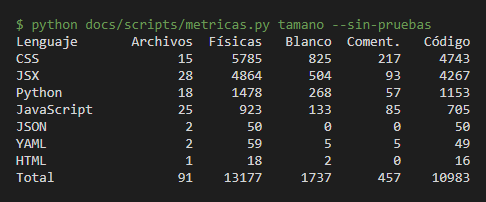
\includegraphics[width=0.48\linewidth]{../evidencias/metricas/script_tamano.png}\hfill
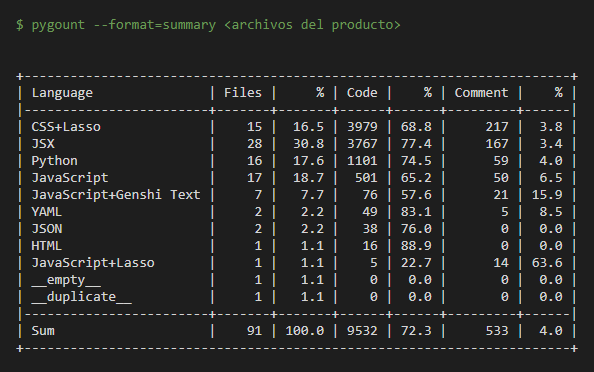
\includegraphics[width=0.48\linewidth]{../evidencias/metricas/pygount_tamano.png}\\[2mm]
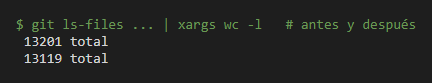
\includegraphics[width=0.48\linewidth]{../evidencias/metricas/wc_tamano.png}
\figurenote{Arriba: \codigo{metricas.py tamano} y pygount; abajo: \codigo{wc -l} (antes y después). Fuente: elaboración propia.}
\end{figure}

\begin{figure}[H]
\centering
\caption{Panel de SonarQube Community 26.7 (antes)}
\label{fig:sonar-tamano}
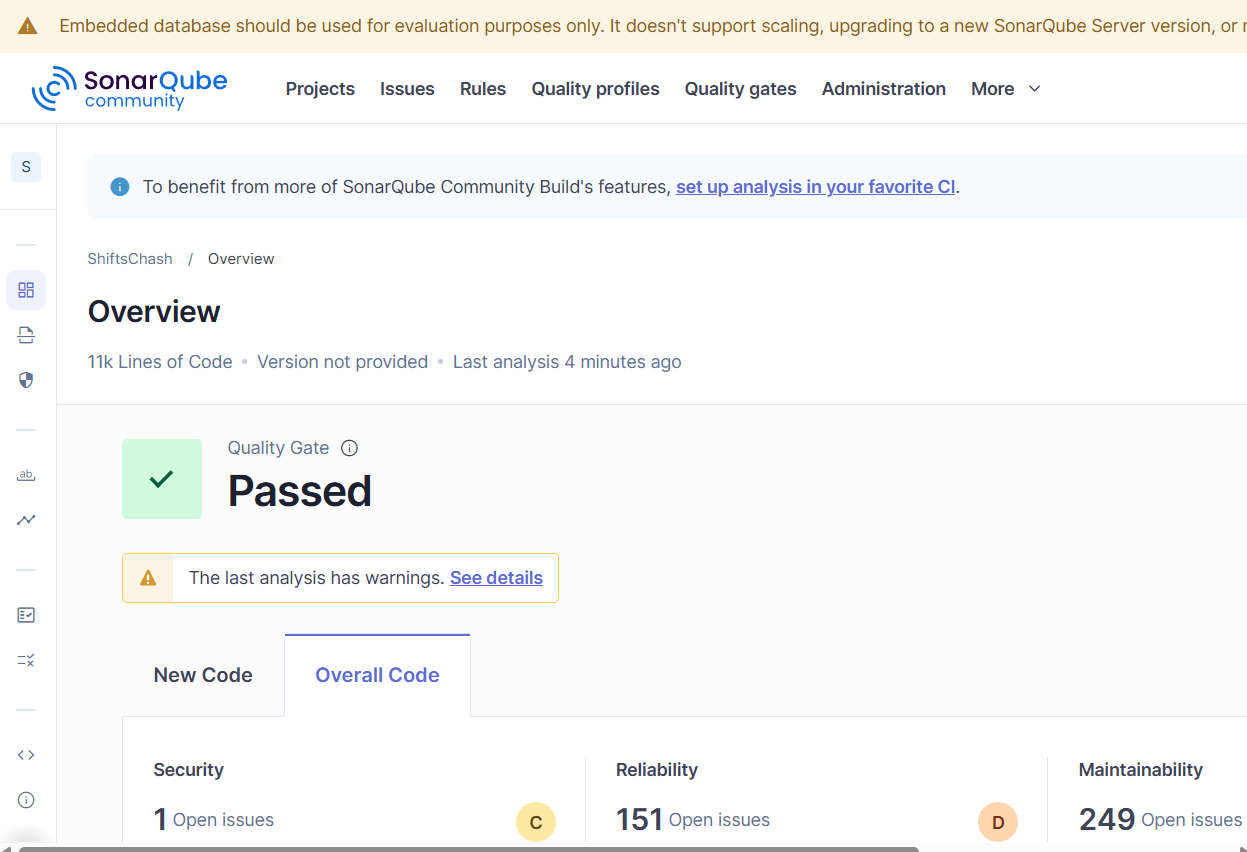
\includegraphics[width=0.8\linewidth]{previo/sonarqube_antes.png}
\figurenote{Fuente: elaboración propia.}
\end{figure}

\paragraph{Análisis.} Las tres herramientas coinciden en el orden de magnitud (entre 9\,500 y 11\,000 líneas de código) y difieren por lo que cada una considera código. El CSS es el 43\,\% del código, lo que refleja el peso de la presentación (tema claro y oscuro, diseño responsivo). La densidad de comentarios del Python bajó de 5,6\,\% a 3,9\,\% porque se borró el código comentado (el login antiguo), no porque se perdieran comentarios útiles; las clases y servicios nuevos tienen docstring.

\subsection{Complejidad ciclomática}

\begin{table}[H]
\caption{Complejidad ciclomática del backend}
\label{tab:complejidad}
\footnotesize
\begin{tabularx}{\linewidth}{L{5.2cm} Y Y}
\toprule
Medida & Antes & Después \\
\midrule
Funciones medidas & 58 & 92 \\
Funciones con $V(G) \leq 10$ \parencite{mccabe1976} & 55 (94,8\,\%) & 92 (100\,\%) \\
Funciones con $V(G) > 10$ & \codigo{update_saving_goal} (14), \codigo{get_date_range} (13), \codigo{update_budget} (13) & Ninguna \\
$V(G)$ máxima & 14 & 8 (\codigo{_toca_hoy}, \codigo{google_auth}) \\
$V(G)$ media & 3,4 & 2,2 \\
\bottomrule
\end{tabularx}
\tablenote{Según el catálogo de \textcite{filo2015}, una función es común con $V(G) \leq 2$, casual hasta 4 y poco común por encima de 4. Fuente: elaboración propia con \codigo{metricas.py complejidad}.}
\end{table}

\begin{table}[H]
\caption{Componentes del frontend con más puntos de decisión (después)}
\label{tab:frontend}
\footnotesize
\begin{tabularx}{\linewidth}{L{4.6cm} Y Y Y}
\toprule
Componente & Líneas & Funciones & Puntos de decisión \\
\midrule
PresupuestoModal.jsx & 466 & 33 & 83 \\
VistaResumen.jsx & 519 & 63 & 80 \\
VistaHistorial.jsx & 311 & 39 & 58 \\
VistaMetas.jsx & 367 & 33 & 46 \\
VistaConfiguracion.jsx & 385 & 24 & 45 \\
VistaPresupuestos.jsx & 409 & 40 & 43 \\
\bottomrule
\end{tabularx}
\tablenote{Puntos de decisión: \codigo{if}, \codigo{for}, \codigo{while}, \codigo{case}, \codigo{catch}, operador ternario, \codigo{\&\&} y \codigo{||}. Los valores son casi iguales a los de antes: la refactorización se concentró en el backend. Fuente: elaboración propia con \codigo{metricas.py frontend}.}
\end{table}

\subsection{Métricas orientadas a clases (suite CK)}

\paragraph{Definiciones aplicadas a Python.} Medimos las clases del backend (entidades SQLAlchemy y esquemas Pydantic) y, como la lógica de negocio está en funciones, también cada \textbf{módulo tratado como una clase}: sus funciones son los métodos y sus nombres globales, los atributos.
\begin{itemize}
  \item \textbf{WMC}: suma de las complejidades ciclomáticas de los métodos.
  \item \textbf{DIT}: profundidad de herencia hasta la clase raíz del marco (\codigo{Base} o \codigo{BaseModel} cuentan como nivel 1).
  \item \textbf{NOC}: número de subclases directas en el proyecto.
  \item \textbf{CBO}: número de otras clases o módulos del proyecto con los que se acopla (referencias o importaciones internas).
  \item \textbf{RFC}: métodos propios más funciones distintas que invocan.
  \item \textbf{LCOM}: pares de métodos sin atributos comunes menos pares con atributos comunes, mínimo 0 \parencite{chidamber1994}.
  \item \textbf{LCOM4}: componentes conexas del grafo de métodos, donde dos métodos se unen si comparten un atributo o uno usa al otro \parencite{hitz1995}. Vale 1 si la unidad es cohesiva.
\end{itemize}

\begin{table}[H]
\caption{Valores de referencia usados}
\label{tab:referencias-ck}
\footnotesize
\begin{tabularx}{\linewidth}{L{1.6cm} L{2.4cm} L{2.6cm} L{2.4cm} Y}
\toprule
Métrica & Común (bueno) & Casual (regular) & Poco común (malo) & Fuente \\
\midrule
WMC & $\leq 11$ & 12–34 & $> 34$ & \textcite{filo2015} \\
DIT & $\leq 2$ & 3–4 & $> 4$ & \textcite{filo2015} \\
NOC & $\leq 1$ & 2–3 & $> 3$ & \textcite{filo2015} (NSC) \\
CBO & $\leq 6$ & 7–16 & $> 16$ & \textcite{filo2015} (acoplamiento eferente) \\
NOM & $\leq 6$ & 7–14 & $> 14$ & \textcite{filo2015} \\
RFC & \multicolumn{3}{l}{Sin umbral numérico: «bajo», comparar con el resto} & \textcite{rosenberg1998} \\
LCOM4 & 1 & \multicolumn{2}{l}{$> 1$: responsabilidades separables} & \textcite{hitz1995} \\
$V(G)$ por función & $\leq 10$ & \multicolumn{2}{l}{$> 10$: dividir la función} & \textcite{mccabe1976} \\
\bottomrule
\end{tabularx}
\tablenote{Los umbrales de \textcite{filo2015} se derivaron de 111 sistemas Java; los usamos como referencia de lo habitual, no como reglas absolutas. Fuente: elaboración propia.}
\end{table}

\begin{table}[H]
\caption{Suite CK de las clases del backend (después)}
\label{tab:ck-clases}
\footnotesize
\begin{tabularx}{\linewidth}{L{3.2cm} L{2.2cm} *{7}{>{\centering\arraybackslash}X}}
\toprule
Clase & Tipo & NOM & WMC & DIT & NOC & CBO & RFC & LCOM4 \\
\midrule
User & Entidad & 0 & 0 & 1 & 0 & 4 & 0 & — \\
Category, Budget, Transaction & Entidad & 0 & 0 & 1 & 0 & 2 & 0 & — \\
SavingGoal & Entidad & 0 & 0 & 1 & 0 & 1 & 0 & — \\
SavingGoalCreate & Esquema & 4 & 10 & 1 & 0 & 0 & 10 & 3 \\
BudgetBase & Esquema & 4 & 5 & 1 & 2 & 0 & 9 & 4 \\
BudgetUpdate & Esquema & 4 & 6 & 1 & 0 & 0 & 9 & 4 \\
BudgetCreate & Esquema & 1 & 5 & 2 & 0 & 0 & 3 & 1 \\
TransactionCreate & Esquema & 3 & 6 & 1 & 0 & 0 & 7 & 3 \\
CategoryCreate, SavingGoalUpdate & Esquema & 2 & 4–5 & 1 & 0 & 0 & 5–6 & 2 \\
Otros 13 esquemas & Esquema & 0–1 & 0–2 & 1–2 & 0 & 0–1 & 0–4 & 0–1 \\
\midrule
Máximo (después / antes) & & 4 / 3 & 10 / 7 & 2 / 2 & 2 / 2 & 4 / 4 & 10 / 7 & 4 / 3 \\
\bottomrule
\end{tabularx}
\tablenote{Las entidades no tienen métodos, por lo que LCOM no aplica. El reporte completo, con LCOM, está en la Figura \ref{fig:ck}. Fuente: elaboración propia con \codigo{metricas.py ck}.}
\end{table}

\begin{table}[H]
\caption{Suite CK de los módulos del backend tratados como clases}
\label{tab:ck-modulos}
\footnotesize
\begin{tabularx}{\linewidth}{L{4.4cm} *{5}{>{\centering\arraybackslash}X} L{3.2cm}}
\toprule
Módulo & NOM & WMC & CBO & RFC & LCOM4 & Antes (NOM / WMC / RFC) \\
\midrule
routes/savings.py & 6 & 7 & 5 & 20 & 1 & 10 / \textbf{50} / 54 \\
routes/budgets.py & 4 & 5 & 5 & 17 & 1 & 6 / \textbf{37} / 35 \\
routes/transactions.py & 6 & 12 & 5 & 28 & 1 & 5 / 13 / 26 \\
routes/profile.py & 7 & 16 & 4 & 32 & 1 & Igual \\
routes/users.py & 3 & 14 & 4 & 23 & 1 & 3 / 16 / 23 \\
routes/categories.py & 4 & 7 & 5 & 19 & 1 & 4 / 6 / 19 \\
services/saving\_service.py & 14 & \textbf{39} & 2 & 63 & 3 & No existía \\
services/budget\_service.py & 12 & 25 & 3 & 40 & 4 & No existía \\
services/category\_service.py & 2 & 3 & 1 & 8 & 1 & No existía \\
auth.py & 4 & 7 & 2 & 20 & 3 & 4 / 8 / 21 \\
scheduler.py & 2 & 12 & 3 & 15 & 1 & Igual \\
\bottomrule
\end{tabularx}
\tablenote{En negrita, los valores poco comunes según \textcite{filo2015} (WMC $> 34$). Fuente: elaboración propia con \codigo{metricas.py ck}.}
\end{table}

\begin{figure}[H]
\centering
\caption{Reporte de la suite CK (después)}
\label{fig:ck}
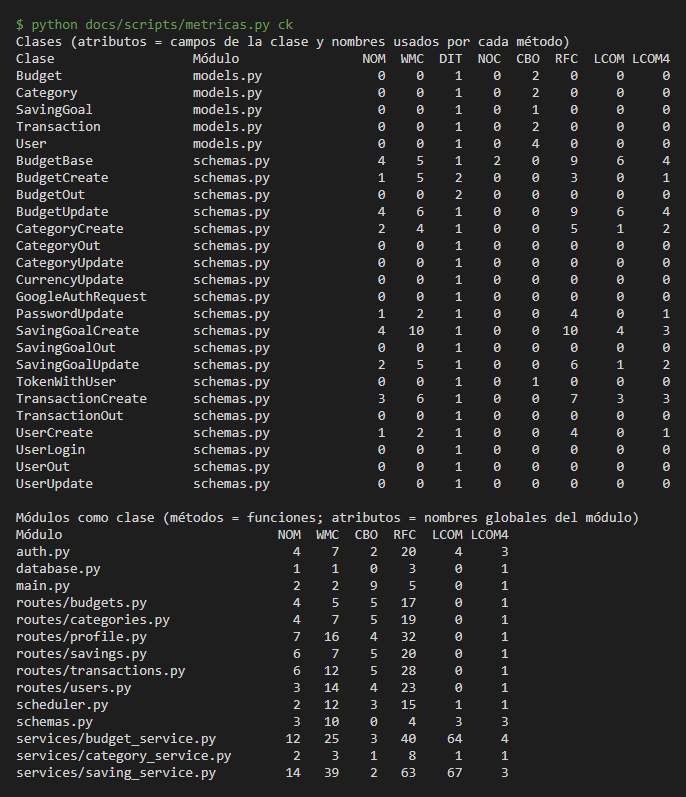
\includegraphics[width=0.75\linewidth]{../evidencias/metricas/ck_despues.png}
\figurenote{Fuente: elaboración propia con \codigo{metricas.py ck}.}
\end{figure}

\subsection{Clases y módulos problemáticos, y mejoras}

\begin{table}[H]
\caption{Hallazgos de las métricas internas y acciones}
\label{tab:hallazgos-internos}
\footnotesize
\begin{tabularx}{\linewidth}{L{3.4cm} L{4.4cm} Y}
\toprule
Unidad & Hallazgo (antes) & Acción y resultado \\
\midrule
routes/savings.py & WMC 50, RFC 54; \codigo{update_saving_goal} con $V(G) = 14$; construcción de \codigo{SavingGoalOut} repetida 3 veces & \textbf{Hecho}: lógica movida a \codigo{saving_service}; WMC 7, RFC 20, ninguna función $> 10$ \\
routes/budgets.py & WMC 37; \codigo{get_date_range} y \codigo{update_budget} con $V(G) = 13$; \codigo{BudgetOut} repetido 3 veces & \textbf{Hecho}: \codigo{budget_service} con un diccionario de períodos; WMC 5; $V(G)$ máxima de 5 \\
Esquemas \codigo{Token} y \codigo{ToggleDayRequest} & Clases sin uso (código muerto) & \textbf{Hecho}: eliminadas \\
services/saving\_service.py & WMC 39 (poco común) y NOM 14 (casual): reúne el cálculo del plan y el acceso a datos de las metas; LCOM4 = 3 & \textbf{Propuesta}: separar el cálculo del plan (\codigo{generate_daily_amounts}, \codigo{calculate_progress} y el redondeo) en un módulo \codigo{saving_plan.py} y dejar en el servicio la persistencia. Ninguna función supera $V(G) = 6$. \\
services/budget\_service.py & LCOM4 = 4: el cálculo del período y del gasto forma un grupo, y \codigo{create_budget}, \codigo{update_budget} y \codigo{get_owned_budget} son independientes & \textbf{Propuesta}: mover los tres a un repositorio de presupuestos si el módulo crece. \\
Validadores (\codigo{BudgetBase}, \codigo{BudgetUpdate}) & LCOM4 = 4: cada validador revisa un campo distinto & Aceptado: es la forma idiomática de Pydantic; cada validador es una sola regla. \\
PresupuestoModal.jsx, VistaResumen.jsx & Más de 80 puntos de decisión; mezclan cálculo y presentación & \textbf{Propuesta}: extraer los cálculos a hooks (\codigo{usePresupuestoForm}, \codigo{useResumen}) como se hizo con \codigo{useTransaccionForm}. \\
\bottomrule
\end{tabularx}
\tablenote{Fuente: elaboración propia.}
\end{table}

\paragraph{Análisis de la calidad del diseño.} La \textbf{modularidad} mejoró: las rutas pasaron de concentrar la lógica (WMC 50 y 37) a ser delgadas (WMC $\leq 16$), y las reglas de negocio están en servicios que se prueban solos. El \textbf{acoplamiento} sigue bajo: el CBO máximo de una clase es 4 y el de un módulo de rutas es 5, dentro del rango común ($\leq 6$); subió en uno porque las rutas ahora dependen de su servicio, un acoplamiento intencional y estable. La \textbf{herencia} es poco profunda (DIT $\leq 2$, NOC $\leq 2$), adecuada para entidades y esquemas. La \textbf{cohesión} es alta en las rutas (LCOM4 = 1) y aceptable en los servicios; el punto a vigilar es \codigo{saving_service}, que conviene dividir como indica la Tabla \ref{tab:hallazgos-internos}.

% =====================================================================
% Tercera parte – 6 y 7. Métricas externas y conclusiones
% =====================================================================
\section{Métricas externas basadas en ISO/IEC 25010}

Cada tabla relaciona la métrica con su requisito no funcional (Tabla \ref{tab:rnf}) y muestra el valor objetivo, el valor antes (25 de octubre de 2026, código \codigo{0efe28b}) y el valor después (21 de noviembre de 2026, rama \codigo{fix/defectos}). La fórmula sigue la forma de ISO/IEC 25023: $X = A/B$, donde $A$ es el número de elementos que cumplen y $B$ el total evaluado \parencite{iso25023}.

\paragraph{Versión de la norma.} Usamos los nombres de ISO/IEC 25010:2011. La versión 2023 renombra algunas características: usabilidad pasa a \emph{capacidad de interacción}, portabilidad a \emph{flexibilidad}, y agrega \emph{seguridad física} (\emph{safety}). Las métricas no cambian con el nombre.

% \metricas{titulo}{etiqueta}{filas}{nota}
\newcommand{\metricas}[4]{%
\begin{table}[H]
\caption{#1}
\label{#2}
\scriptsize
\begin{tabularx}{\linewidth}{L{2cm} Y L{1.1cm} L{1.5cm} L{1.7cm} L{1.9cm}}
\toprule
Subcaract. & Métrica y fórmula & RNF & Objetivo & Antes & Después \\
\midrule
#3
\bottomrule
\end{tabularx}
\tablenote{#4}
\end{table}}

\subsection{Adecuación funcional}

\metricas{Métricas de adecuación funcional}{tab:me-funcional}{%
Completitud & RF implementados: $1 - \frac{\text{RF sin implementar}}{20}$ & — & 1,00 & 1,00 & 1,00 \\
Corrección & RF sin defectos abiertos: $1 - \frac{\text{RF con defecto}}{20}$ & RNF08 & 1,00 & 0,90 (RF12 por D-04 y RF16 por D-01) & 1,00 \\
Corrección & Cálculos correctos en las pruebas: $\frac{\text{aprobadas}}{\text{ejecutadas}}$ & RNF08 & 1,00 & 48/49 = 0,98 & 58/58 = 1,00 \\
Pertinencia & Servicios anunciados disponibles: $\frac{\text{disponibles}}{\text{anunciados}}$ & — & 1,00 & 3/3 = 1,00 & 3/3 = 1,00 \\
Aceptación & RF aceptados por el usuario final & — & $\geq 0{,}90$ & No medido & \resRFAceptados \\
}{Herramientas: pytest, Cypress y Selenium (Segunda parte). Fuente: elaboración propia.}

\subsection{Eficiencia de desempeño}

\metricas{Métricas de eficiencia de desempeño}{tab:me-desempeno}{%
Comportamiento temporal & Percentil 90 del tiempo de respuesta con 50 usuarios & RNF11 & $< 2$ s & 10 ms (local, solo GET, 30 s de rampa) & 22 ms (local, GET y POST, 60 s); Render: \resJmeterRender \\
Comportamiento temporal & Tasa de error bajo carga: $\frac{\text{errores}}{\text{peticiones}}$ & RNF11 & $< 1$\,\% & 0\,\% (66,7\,\% con datos inválidos) & 0\,\% (0/1\,500) \\
Comportamiento temporal & LCP de la portada, perfil móvil (4G simulado) & RNF15 & $\leq 2{,}5$ s & 6,89 s (Vercel) & 4,43 s (versión corregida) \\
Comportamiento temporal & LCP de la portada, perfil de escritorio & RNF15 & $\leq 2{,}5$ s & 2,10 s (Vercel) & 1,40 s (versión corregida) \\
Utilización de recursos & Puntaje de rendimiento de Lighthouse (móvil / escritorio) & RNF15 & $\geq 90$ & 59 / 77 & 75 / 90 \\
Utilización de recursos & JavaScript que descarga la portada & — & Mínimo & Un solo paquete de más de 500 kB & 292 kB (el dashboard, 492 kB, se carga al entrar) \\
}{Herramientas: Apache JMeter 5.6.3 y Lighthouse 12.8.2. «Antes» en Lighthouse es la aplicación desplegada en Vercel con el código anterior; «después» es la compilación de producción de la rama, servida en local con \codigo{vite preview}. Fuente: elaboración propia.}

\begin{figure}[H]
\centering
\caption{Lighthouse en perfil móvil: antes (Vercel) y después (versión corregida)}
\label{fig:lighthouse}
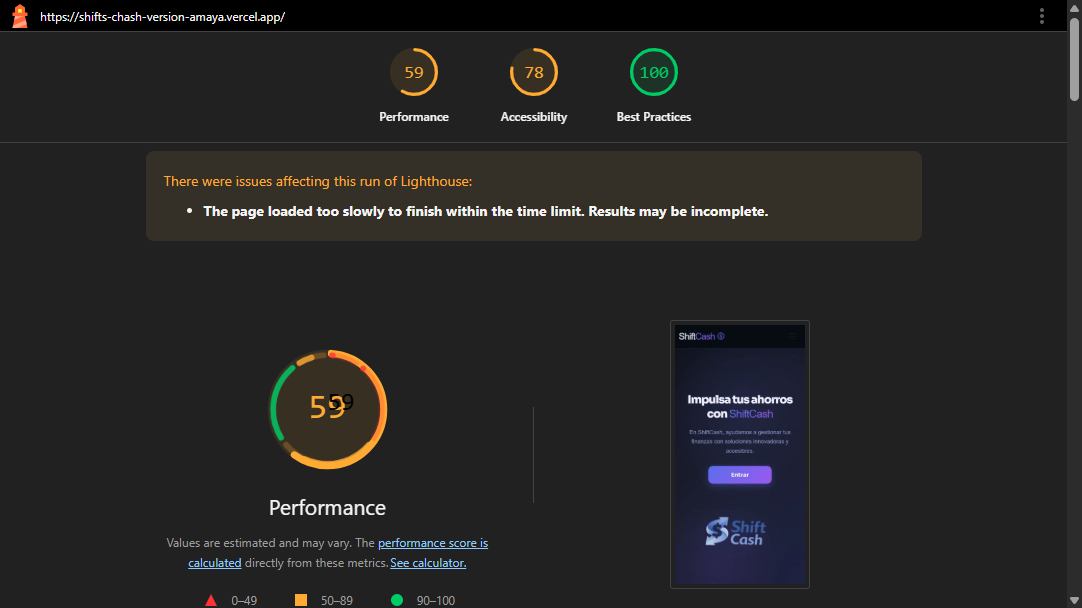
\includegraphics[width=0.49\linewidth]{../evidencias/lighthouse/vercel.png}\hfill
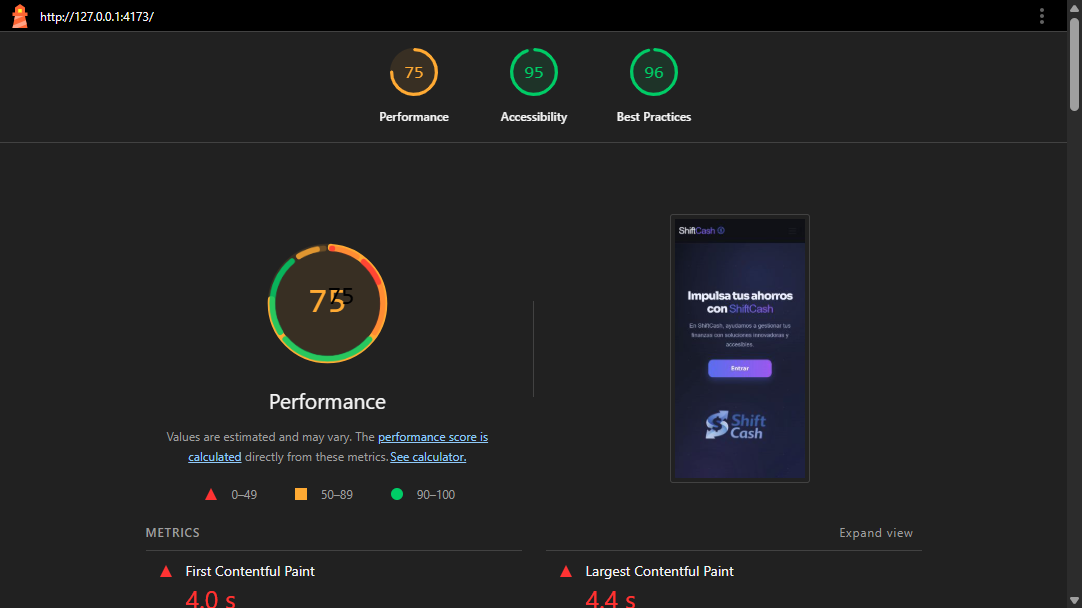
\includegraphics[width=0.49\linewidth]{../evidencias/lighthouse/local.png}
\figurenote{Fuente: elaboración propia con Lighthouse 12.8.2.}
\end{figure}

\paragraph{Mejoras aplicadas.} La portada descargaba todo el código del dashboard (incluido Recharts) y un logotipo PNG de 297 kB y 1500 × 1000 px. Cargamos el dashboard con \codigo{React.lazy} y reemplazamos el logotipo por un WebP de 29 kB a 750 × 500 px. El LCP en perfil de escritorio cumple el objetivo; en perfil móvil bajó de 6,9 a 4,4 s, todavía por encima de 2,5 s, porque el contenido se dibuja después de cargar las hojas de estilo y fuentes externas (Bootstrap y Google Fonts) y de ejecutar React.

\subsection{Compatibilidad}

\metricas{Métricas de compatibilidad}{tab:me-compatibilidad}{%
Interoperabilidad & Routers con contrato REST/JSON publicado en OpenAPI & — & 1,00 & 6/6 = 1,00 & 6/6 = 1,00 \\
Interoperabilidad & Integraciones externas operativas: $\frac{\text{operativas}}{\text{declaradas en la interfaz}}$ & — & 1,00 & 1/2 = 0,50 (Facebook sin implementar) & 1/2 = 0,50 \\
Coexistencia & Servicios que se despliegan y escalan por separado & — & 1,00 & 3/3 (Vercel, Render, Supabase) & 3/3 \\
}{Herramientas: \codigo{/openapi.json} de FastAPI e inspección de la interfaz. Fuente: elaboración propia.}

\subsection{Usabilidad}

\metricas{Métricas de usabilidad}{tab:me-usabilidad}{%
Accesibilidad & Puntaje de accesibilidad de Lighthouse (móvil) & RNF14 & $\geq 90$ & 78 & 95 \\
Accesibilidad & Campos con etiqueta asociada en el formulario de contacto & RNF14 & 1,00 & 0/3 = 0,00 & 3/3 = 1,00 \\
Accesibilidad & Botones con nombre accesible en la portada & RNF14 & 1,00 & Menú sin nombre & 1,00 (\codigo{aria-label}) \\
Operabilidad & Mediana del tiempo para registrar un gasto (PU-06) & RNF07 & $\leq 60$ s & No medido & \resPUMediana{} s \\
Operabilidad & Tasa de éxito al primer intento (PU-06) & RNF07 & $\geq 0{,}90$ & No medido & \resPUExito \\
Protección frente a errores & Errores de validación de la API mostrados como texto legible & RNF05 & 1,00 & 0 (un 422 rompía el formulario, D-13) & 1,00 \\
}{Lighthouse marca aún el contraste de un texto de la portada (\codigo{text-primary}). Fuente: elaboración propia.}

\subsection{Fiabilidad}

\metricas{Métricas de fiabilidad}{tab:me-fiabilidad}{%
Madurez & Pruebas automatizadas sin fallos: $\frac{\text{aprobadas}}{\text{ejecutadas}}$ & — & 1,00 & 48/49 = 0,98 & 95/95 = 1,00 \\
Disponibilidad & Tiempo operativo del frontend en la ventana de prueba & RNF10 & $\geq 0{,}99$ & 1,00 & 1,00 \\
Disponibilidad & Tiempo operativo de la API en la ventana de prueba & RNF10 & $\geq 0{,}99$ & 0,00 (más de 7 min sin respuesta) & \resDisponibilidadApi \\
Tolerancia a fallos & Entradas inválidas respondidas con 4xx: $\frac{\text{4xx}}{\text{entradas inválidas probadas}}$ & RNF05 & 1,00 & 4/6 = 0,67 & 5/5 = 1,00 (la meta sin fecha final ahora es una entrada válida) \\
Recuperabilidad & Recurrentes que no se duplican al reejecutar el programador & — & 1,00 & No ejecutado & 1,00 (PI-08) \\
}{Herramientas: pytest, Cypress y observación del servicio. Fuente: elaboración propia.}

\subsection{Seguridad}

\metricas{Métricas de seguridad}{tab:me-seguridad}{%
Autenticidad & Endpoints de datos que exigen JWT: $\frac{\text{protegidos}}{\text{de datos}}$ & RNF02 & 1,00 & 26/26 = 1,00 & 26/26 = 1,00 \\
Confidencialidad & Contraseñas guardadas con hash: $\frac{\text{con hash}}{\text{guardadas}}$ & RNF01 & 1,00 & 1,00 & 1,00 \\
Confidencialidad & Credenciales escritas en el código & RNF13 & 0 & 2 (D-06) & 0 \\
Confidencialidad & Registros ajenos visibles o modificables & RNF12 & 0 & 0 (estático) & 0 (ejecutado) \\
Integridad & Campos críticos validados en el servidor (F1–F3): $\frac{\text{validados}}{14}$ & RNF05 & 1,00 & 9/14 = 0,64 & 14/14 = 1,00 \\
Integridad & Orígenes no autorizados que reciben cabeceras CORS & RNF03 & 0 & 0 (estático) & 0 (ejecutado) \\
Resistencia & Alertas de ZAP de riesgo alto / medio & RNF13 & 0 / 0 & 0 / 3 & \resZapResumen \\
}{Los 14 campos críticos son: en transacciones, monto mínimo, monto máximo, tipo, categoría y frecuencia; en presupuestos, monto, período, mes, año y fechas del período único; en metas, nombre, objetivo, fecha final y orden de fechas. La frecuencia se validó al corregir D-14. Fuente: elaboración propia.}

\subsection{Mantenibilidad}

\metricas{Métricas de mantenibilidad}{tab:me-mantenibilidad}{%
Analizabilidad & Funciones con $V(G) \leq 10$: $\frac{A}{B}$ & RNF09 & 1,00 & 55/58 = 0,95 & 92/92 = 1,00 \\
Analizabilidad & Densidad de comentarios del Python & — & — & 93/1\,657 = 0,056 & 57/1\,478 = 0,039 \\
Modularidad & CBO medio de los routers & — & $\leq 6$ & 4,0 & 4,7 \\
Reusabilidad & Construcciones de respuesta duplicadas & — & 0 & 6 & 0 \\
Modificabilidad & Elementos de código muerto & — & 0 & 3 & 0 \\
Capacidad de prueba & Cobertura de líneas del backend & RNF09 & $\geq 0{,}80$ & 0,00 & 0,95 \\
}{Herramientas: \codigo{metricas.py}, pytest-cov y SonarQube (antes: mantenibilidad A, 249 incidencias; después: \resSonar). Fuente: elaboración propia.}

\subsection{Portabilidad}

\metricas{Métricas de portabilidad}{tab:me-portabilidad}{%
Adaptabilidad & Resoluciones sin desbordamiento: $\frac{\text{correctas}}{\text{probadas}}$ & RNF06 & 1,00 & 2/2 & 2/2 \\
Adaptabilidad & Navegadores verificados: $\frac{\text{correctos}}{4}$ (Chrome, Firefox, Edge, Safari) & RNF06 & 1,00 & 2/4 = 0,50 & \resNavegadores \\
Instalabilidad & Pasos de instalación documentados: $\frac{\text{en el README}}{\text{necesarios}}$ & — & 1,00 & 3/6 = 0,50 & 6/6 = 1,00 \\
}{Los seis pasos son: clonar, instalar y configurar el backend (\codigo{.env}), levantar la API, instalar el frontend, configurar \codigo{.env.local} y levantar el frontend. Fuente: elaboración propia.}

\section{Conclusiones de la medición}

\paragraph{Calidad interna.} La refactorización redujo la complejidad sin aumentar el tamaño: el código de lógica bajó de 6\,228 a 6\,125 líneas, ninguna función supera $V(G) = 10$ (antes, tres), la complejidad media bajó de 3,4 a 2,2 y las rutas pasaron de WMC 50 y 37 a 7 y 5. El acoplamiento y la herencia siguen en los rangos comunes del catálogo de \textcite{filo2015}. El único valor poco común es el WMC de \codigo{saving_service} (39), que proponemos dividir.

\paragraph{Calidad externa.} Mejoraron la corrección funcional (0,90 → 1,00), la integridad de las entradas (0,64 → 1,00), la tolerancia a fallos (0,67 → 1,00), la accesibilidad (78 → 95), la instalabilidad (0,50 → 1,00) y la capacidad de prueba (cobertura de 0 a 95\,\%). Siguen por debajo del objetivo el LCP en perfil móvil (4,4 s frente a 2,5 s) y la verificación en Edge y Safari, y faltan por medir la disponibilidad de la API en Render, la tarea PU-06 y los nuevos escaneos de ZAP y SonarQube.


% ===================== CUARTA PARTE =====================
\newpage
\part*{Cuarta parte: estimación del software}
\addcontentsline{toc}{part}{Cuarta parte: estimación del software}
\setcounter{section}{0}
% =====================================================================
% Cuarta parte – Estimación del software
% =====================================================================
\section{Supuestos comunes}

Para comparar los modelos usamos los mismos supuestos. Todos los cálculos se reproducen con \codigo{docs/scripts/estimacion.py} (Apéndice \ref{ap:estimacion}).

\begin{itemize}
  \item Una persona-mes (PM) equivale a 160 horas.
  \item Cuando el modelo no da el tiempo de desarrollo, se calcula con la ecuación de calendario de COCOMO, $T = 2{,}5 \cdot E^{0{,}38}$ meses, y el número de personas con $P = E/T$ \parencite{boehm2000}.
  \item El costo de una persona-mes sale de una tarifa justificada (sección \ref{sec:presupuesto}): \$6\,646\,961.
\end{itemize}

\section{Puntos de función}

Conteo IFPUG \parencite{albrecht1979,ifpug2010} sobre el sistema completo.

\begin{table}[H]
\caption{Conteo de puntos de función no ajustados}
\label{tab:pf}
\footnotesize
\begin{tabularx}{\linewidth}{L{1cm} Y L{1.4cm} L{0.8cm} L{0.8cm}}
\toprule
Tipo & Elementos identificados & Complejidad & Peso & PF \\
\midrule
ILF & users, category, budget, transactions, saving\_goal (5) & Baja & 7 & 35 \\
EIF & Google userinfo (1) & Baja & 5 & 5 \\
EI & Crear y actualizar transacción, presupuesto y meta (6) & Media & 4 & 24 \\
EI & Registro, login, Google, perfil, contraseña, moneda, subir y eliminar foto, eliminar cuenta, eliminar transacción, CRUD de categoría (3), eliminar presupuesto, eliminar meta, marcar día (16) & Baja & 3 & 48 \\
EO & Presupuestos con gasto y porcentaje, progreso de metas, resumen, recurrentes automáticas (4) & Media & 5 & 20 \\
EO & Gráficas de torta, barras y áreas (1) & Alta & 7 & 7 \\
EQ & Historial, categorías, \codigo{/users/me}, detalle de meta (4) & Baja & 3 & 12 \\
\midrule
\multicolumn{4}{l}{Puntos de función no ajustados (PFNA)} & 151 \\
\bottomrule
\end{tabularx}
\tablenote{Fuente: elaboración propia.}
\end{table}

\begin{table}[H]
\caption{Características generales del sistema}
\label{tab:gsc}
\footnotesize
\begin{tabularx}{\linewidth}{Y L{1cm} Y L{1cm}}
\toprule
Característica & Valor & Característica & Valor \\
\midrule
Comunicación de datos & 4 & Actualización en línea & 4 \\
Procesamiento distribuido & 3 & Procesamiento complejo & 2 \\
Rendimiento & 2 & Reutilización & 2 \\
Configuración muy utilizada & 2 & Facilidad de instalación & 2 \\
Tasa de transacciones & 2 & Facilidad de operación & 3 \\
Entrada de datos en línea & 5 & Múltiples sitios & 3 \\
Eficiencia del usuario final & 4 & Facilidad de cambio & 3 \\
\midrule
\multicolumn{3}{l}{Total (TDI)} & 41 \\
\bottomrule
\end{tabularx}
\tablenote{Fuente: elaboración propia.}
\end{table}

\begin{align*}
VAF &= 0{,}65 + 0{,}01 \times 41 = 1{,}06 & PF &= 151 \times 1{,}06 = 160{,}06\\
E &= 160{,}06 \times 8\ \text{h/PF} = 1\,280\ \text{h} = 8{,}00\ \text{PM} & T &= 2{,}5 \times 8{,}00^{0{,}38} = 5{,}51\ \text{meses}\\
& & P &= 8{,}00 / 5{,}51 = 1{,}45
\end{align*}

La productividad de 8 horas por punto de función es un supuesto típico para desarrollo web con lenguajes de alto nivel.

\section{Puntos de función COSMIC}

El método COSMIC (ISO/IEC 19761) mide el tamaño funcional contando los \textbf{movimientos de datos} de cada proceso funcional: entradas (E) y salidas (X) que cruzan la frontera con un usuario funcional, y lecturas (R) y escrituras (W) en el almacenamiento persistente. Cada movimiento vale 1 CFP (\emph{COSMIC Function Point}). Los usuarios funcionales son el usuario de la aplicación, el servicio de Google y el reloj del programador de tareas; los grupos de datos son usuario, categoría, presupuesto, transacción y meta. Contamos un movimiento por grupo de datos y una salida para los mensajes de confirmación o error de cada proceso.

\begin{table}[H]
\caption{Conteo COSMIC por proceso funcional}
\label{tab:cosmic}
\scriptsize
\setlength{\tabcolsep}{3pt}
\begin{tabularx}{\linewidth}{Y *{5}{c} | Y *{5}{c}}
\toprule
Proceso & E & X & R & W & CFP & Proceso & E & X & R & W & CFP \\
\midrule
Registrar usuario & 1 & 1 & 1 & 1 & 4 & Iniciar sesión & 1 & 2 & 1 & 0 & 4 \\
Iniciar sesión con Google & 2 & 3 & 1 & 1 & 7 & Consultar perfil & 1 & 1 & 1 & 0 & 3 \\
Editar perfil & 1 & 1 & 1 & 1 & 4 & Cambiar contraseña & 1 & 1 & 1 & 1 & 4 \\
Cambiar moneda & 1 & 1 & 1 & 1 & 4 & Subir foto de perfil & 1 & 1 & 1 & 1 & 4 \\
Eliminar foto de perfil & 1 & 1 & 1 & 1 & 4 & Eliminar cuenta y sus datos & 1 & 1 & 1 & 5 & 8 \\
Listar categorías & 1 & 1 & 1 & 0 & 3 & Crear categoría & 1 & 1 & 1 & 1 & 4 \\
Editar categoría & 1 & 1 & 1 & 1 & 4 & Eliminar categoría & 1 & 1 & 2 & 2 & 6 \\
Registrar transacción & 1 & 1 & 1 & 1 & 4 & Consultar historial con filtros & 1 & 1 & 2 & 0 & 4 \\
Editar transacción & 1 & 1 & 2 & 1 & 5 & Eliminar transacción & 1 & 1 & 1 & 1 & 4 \\
Crear presupuesto & 1 & 1 & 1 & 1 & 4 & Consultar presupuestos con gasto & 1 & 1 & 3 & 0 & 5 \\
Editar presupuesto & 1 & 1 & 2 & 1 & 5 & Eliminar presupuesto & 1 & 1 & 1 & 1 & 4 \\
Crear meta con plan diario & 1 & 1 & 1 & 1 & 4 & Consultar metas y progreso & 1 & 1 & 1 & 0 & 3 \\
Editar meta & 1 & 1 & 2 & 1 & 5 & Eliminar meta & 1 & 1 & 1 & 1 & 4 \\
Marcar o desmarcar día & 1 & 1 & 1 & 1 & 4 & Ver resumen del mes & 1 & 1 & 2 & 0 & 4 \\
Ver gráficas & 1 & 1 & 2 & 0 & 4 & Generar recurrentes (reloj) & 1 & 0 & 1 & 1 & 3 \\
\midrule
\multicolumn{6}{l|}{Totales: E = 31, X = 32, R = 39, W = 27} & \multicolumn{6}{l}{\textbf{Tamaño: 129 CFP}} \\
\bottomrule
\end{tabularx}
\vspace{6pt}
\tablenote{Los 30 procesos cubren los 20 RF. «Eliminar cuenta» escribe en los cinco grupos de datos por la eliminación en cascada (D-11); «Eliminar categoría» lee las transacciones para impedir el borrado (D-05). Fuente: elaboración propia.}
\end{table}

Para que la comparación con IFPUG dependa solo del tamaño, usamos la misma productividad supuesta, 8 horas por unidad:
\[
E = \frac{129 \times 8}{160} = 6{,}45\ \text{PM} \qquad T = 2{,}5 \times 6{,}45^{0{,}38} = 5{,}08\ \text{meses} \qquad P = \frac{6{,}45}{5{,}08} = 1{,}27
\]
con un costo de talento humano de $6{,}45 \times \$6\,646\,961 = \$42\,872\,896$. COSMIC da un tamaño menor que IFPUG (129 frente a 160 unidades) porque no pondera la complejidad de cada función ni aplica el factor de ajuste: cuenta solo movimientos de datos.

\section{Puntos de casos de uso}

Método de \textcite{karner1993} sobre los 14 casos de uso de la Figura \ref{fig:cu-general}.

\begin{table}[H]
\caption{Peso de los actores y de los casos de uso}
\label{tab:pcu}
\footnotesize
\begin{tabularx}{\linewidth}{L{2.6cm} Y L{0.8cm} L{0.9cm}}
\toprule
Elemento & Detalle & Peso & Total \\
\midrule
Actor complejo & Usuario (interfaz gráfica) & 3 & 3 \\
Actor medio & Google OAuth (protocolo HTTP) & 2 & 2 \\
Actor simple & Programador de tareas (API interna) & 1 & 1 \\
\multicolumn{3}{l}{UAW} & 6 \\
\midrule
CU simples (3) & CU04 Registrarse, CU05 Iniciar sesión, CU08 Editar o eliminar transacción & 5 & 15 \\
CU medios (9) & CU01, CU06, CU07, CU09, CU10, CU11, CU12, CU13, CU14 & 10 & 90 \\
CU complejos (2) & CU02 Gestionar presupuesto, CU03 Gestionar meta & 15 & 30 \\
\multicolumn{3}{l}{UUCW} & 135 \\
\bottomrule
\end{tabularx}
\tablenote{Fuente: elaboración propia.}
\end{table}

Los factores técnicos T1 a T13 valen 3, 3, 3, 2, 1, 1, 3, 3, 4, 2, 1, 0 y 1, que con sus pesos dan $TF = 31$. Los factores de entorno E1 a E8 valen 3, 2, 3, 4, 4, 3, 1 y 1, que dan $EF = 18{,}5$.
\begin{align*}
UUCP &= 6 + 135 = 141 & TCF &= 0{,}6 + 0{,}01 \times 31 = 0{,}91\\
ECF &= 1{,}4 - 0{,}03 \times 18{,}5 = 0{,}845 & UCP &= 141 \times 0{,}91 \times 0{,}845 = 108{,}42\\
E &= 108{,}42 \times 20\ \text{h} = 13{,}55\ \text{PM} & T &= 6{,}73\ \text{meses};\ P = 2{,}01
\end{align*}

\section{Puntos de objeto}

Modelo de composición de aplicaciones de COCOMO II \parencite{boehm2000}.

\begin{table}[H]
\caption{Conteo de puntos de objeto}
\label{tab:po}
\footnotesize
\begin{tabularx}{\linewidth}{L{3.2cm} Y L{0.8cm} L{0.9cm}}
\toprule
Tipo & Objetos & Peso & Total \\
\midrule
Pantallas simples (4) & Home, CategoriaFormModal, ConfirmarEliminar, ConfirmarEliminarCategoria & 1 & 4 \\
Pantallas medias (7) & AuthPage, Historial, Categorías, Configuración, ModalTransaccion, DetalleTransaccion, MetaFormModal & 2 & 14 \\
Pantallas difíciles (5) & Resumen, Gráficas, Presupuestos, Metas (reto), PresupuestoModal & 3 & 15 \\
Componentes 3GL (8) & Módulos de rutas y autenticación del backend, programador & 10 & 80 \\
\midrule
\multicolumn{3}{l}{Puntos de objeto (PO)} & 113 \\
\bottomrule
\end{tabularx}
\tablenote{Fuente: elaboración propia.}
\end{table}

\[
NOP = 113 \times (1 - 0{,}20) = 90{,}4 \qquad E = \frac{90{,}4}{13} = 6{,}95\ \text{PM} \qquad T = 5{,}22\ \text{meses};\ P = 1{,}33
\]
con 20\,\% de reúso (React, Recharts y FastAPI) y productividad nominal de 13 NOP por persona-mes.

\section{Puntos de historia}

Las historias de usuario corresponden a los requisitos funcionales y se estimaron con la serie de Fibonacci \parencite{cohn2005}.

\begin{table}[H]
\caption{Historias de usuario y puntos de historia}
\label{tab:ph}
\footnotesize
\begin{tabularx}{\linewidth}{L{1.1cm} Y L{1.6cm} L{0.8cm}}
\toprule
ID & Como usuario, quiero\ldots & RF & PH \\
\midrule
HU01 & registrarme e iniciar sesión (también con Google) & RF01, RF02 & 5 \\
HU02 & registrar un ingreso o un gasto & RF03 & 5 \\
HU03 & programar transacciones recurrentes & RF04, RF05 & 8 \\
HU04 & editar y eliminar transacciones & RF06 & 3 \\
HU05 & consultar el historial con filtros & RF07 & 5 \\
HU06 & ver el resumen financiero del mes & RF08 & 5 \\
HU07 & ver gráficas de mis movimientos & RF09 & 8 \\
HU08 & gestionar categorías propias & RF10 & 5 \\
HU09 & crear presupuestos con 4 tipos de período & RF11, RF13 & 13 \\
HU10 & ver el gasto ejecutado y las alertas & RF12, RF14 & 8 \\
HU11 & crear metas con un plan de ahorro diario & RF15, RF16, RF18 & 13 \\
HU12 & marcar los días del reto y ver el progreso & RF17 & 5 \\
HU13 & configurar el perfil, la moneda y la foto & RF19 & 3 \\
HU14 & cambiar el tema claro u oscuro & RF20 & 2 \\
HU15 & ver una página informativa pública & — & 1 \\
\midrule
\multicolumn{3}{l}{Total} & 89 \\
\bottomrule
\end{tabularx}
\tablenote{Fuente: elaboración propia.}
\end{table}

Con una velocidad supuesta de 20 puntos por sprint de 2 semanas: $89/20 = 4{,}45$ sprints, es decir, 8,9 semanas o $T = 2{,}05$ meses; con los 3 desarrolladores, $E = 2{,}05 \times 3 = 6{,}16$ PM. En la entrega anterior se supusieron 2 personas; el equipo real tuvo 3.

\section{Estimación con herramienta: COCOMO II}

Se usó la calculadora en línea de COCOMO II (modelo post-arquitectura, COCOMO II.2000) de Ray Madachy \parencite{boehm2000} y se verificó con el script. La entrada es el tamaño de la lógica del producto como se desarrolló (Python, JavaScript y JSX del commit \codigo{0efe28b}): 6\,228 SLOC según la medición de la Tercera parte (la entrega anterior usó 6\,154 con la versión previa del script).

\begin{align*}
E_{esc} &= 0{,}91 + 0{,}01 \textstyle\sum SF = 0{,}91 + 0{,}01 \times 18{,}97 = 1{,}0997 \quad \text{(factores de escala nominales)}\\
EAF &= \textstyle\prod EM = 0{,}866\\
&\quad (\text{DOCU } 0{,}91;\ \text{PVOL } 0{,}87;\ \text{APEX } 1{,}10;\ \text{PLEX } 1{,}09;\ \text{LTEX } 1{,}09;\ \text{TOOL } 0{,}90;\ \text{SITE } 0{,}93)\\
PM &= 2{,}94 \times 6{,}228^{1{,}0997} \times 0{,}866 = 19{,}03\\
T_{DEV} &= 3{,}67 \times 19{,}03^{0{,}28 + 0{,}2(1{,}0997 - 0{,}91)} = 9{,}36\ \text{meses};\quad P = 19{,}03 / 9{,}36 = 2{,}03
\end{align*}

\begin{figure}[H]
\centering
\caption{Calculadora COCOMO II con la entrada de 6\,154 SLOC de la entrega anterior: 18,8 PM y 9,3 meses}
\label{fig:cocomo}
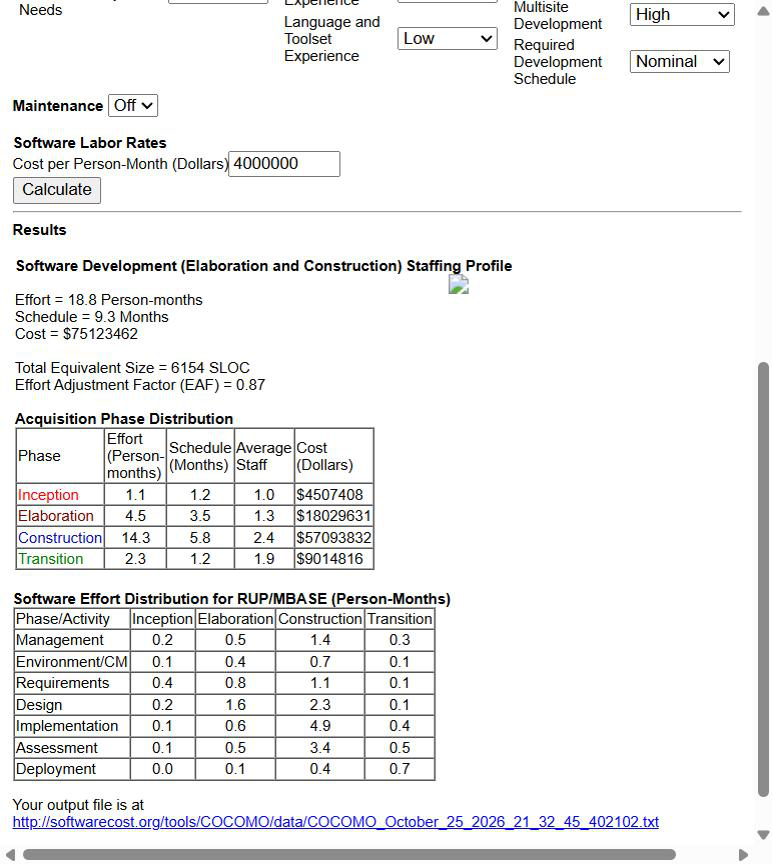
\includegraphics[width=0.75\linewidth, height=0.35\textheight, keepaspectratio]{previo/cocomo_calculadora.png}
\figurenote{Con 6\,228 SLOC el script da 19,03 PM y 9,36 meses (Figura \ref{fig:estimacion-script}). Fuente: elaboración propia.}
\end{figure}

\begin{figure}[H]
\centering
\caption{Recálculo de los seis modelos paramétricos y del presupuesto con \codigo{estimacion.py}}
\label{fig:estimacion-script}
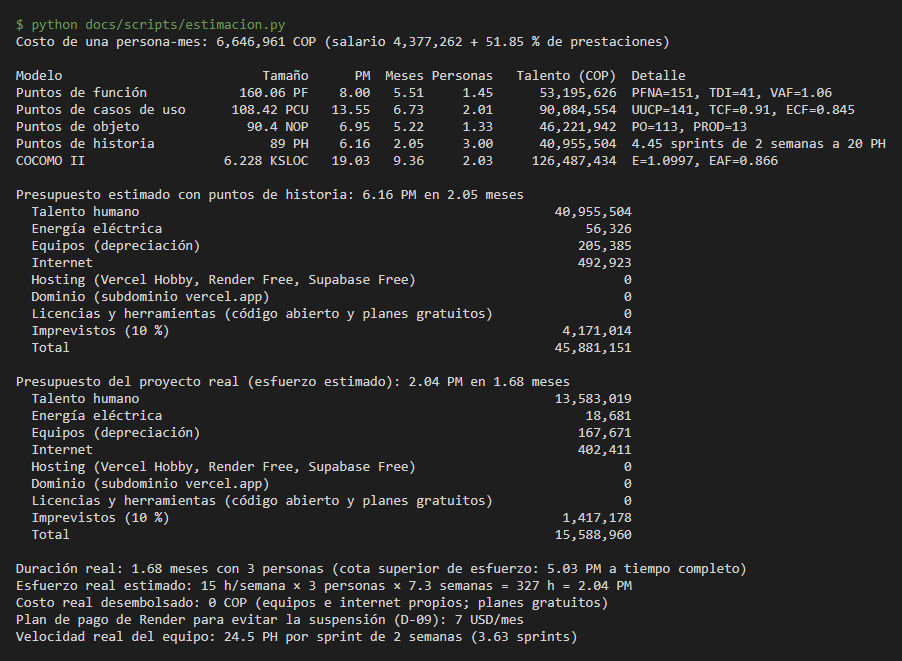
\includegraphics[width=\linewidth]{../evidencias/estimacion_salida.png}
\figurenote{Fuente: elaboración propia.}
\end{figure}

\section{Estimación con una herramienta de inteligencia artificial}

Usamos el asistente \textbf{Claude Opus 5.5} (Anthropic) el 26 de noviembre de 2026. Le dimos la descripción del proyecto y le pedimos una estimación de esfuerzo, tiempo y personas, sin mostrarle los resultados de los otros modelos.

\paragraph{Instrucción (prompt).} «Estima el esfuerzo en personas-mes, la duración en meses y el número de personas para desarrollar esta aplicación web: frontend en React 19 con Vite y backend en FastAPI con SQLAlchemy y PostgreSQL; 20 requisitos funcionales (registro e inicio de sesión con correo y Google, transacciones con recurrencia, historial con filtros, resumen y gráficas, categorías propias, presupuestos con cuatro tipos de período y alertas, metas de ahorro con plan diario y días marcables, perfil, moneda y tema); 5 tablas; despliegue en Vercel, Render y Supabase; pruebas unitarias, de integración y de aceptación. Equipo de 3 estudiantes. Explica cómo llegas al resultado.»

\paragraph{Respuesta resumida.} El asistente estimó por descomposición de tareas (ascendente), en horas de un desarrollador junior:

\begin{table}[H]
\caption{Estimación de la herramienta de IA por módulo}
\label{tab:ia}
\footnotesize
\begin{tabularx}{\linewidth}{Y r}
\toprule
Módulo & Horas \\
\midrule
Autenticación (correo, Google, JWT) & 80 \\
Transacciones, recurrencia e historial con filtros & 140 \\
Categorías propias & 40 \\
Presupuestos con períodos y alertas & 130 \\
Metas de ahorro con plan diario & 120 \\
Resumen y gráficas & 100 \\
Perfil, moneda, foto y tema & 60 \\
Despliegue y configuración & 50 \\
Pruebas & 160 \\
\midrule
\textbf{Total} & \textbf{880 h = 5,5 PM} \\
\bottomrule
\end{tabularx}
\tablenote{Fuente: respuesta de Claude Opus 5.5, organizada por el equipo.}
\end{table}

Propuso una duración de \textbf{2,5 meses}, con $P = 5{,}5 / 2{,}5 = 2{,}2$ personas a tiempo completo, y un costo de talento humano de $5{,}5 \times \$6\,646\,961 = \$36\,558\,284$. La herramienta advirtió que su estimación depende de la experiencia del equipo y que debe calibrarse con datos propios, igual que los modelos paramétricos.

\section{Presupuesto}\label{sec:presupuesto}

\paragraph{Tarifa del talento humano.} Tomamos como salario de un desarrollador junior 2,5 salarios mínimos: según el Observatorio Laboral para la Educación, el 65,6\,\% de los graduados de programas TIC (programación, sistemas, desarrollo de software) gana más de 2,5 salarios mínimos en su primer empleo \parencite{barona2026}. Con el salario mínimo de 2026, \$1\,750\,905 \parencite{decreto1470}, el salario es de \$4\,377\,262. A ese valor sumamos la carga prestacional de ley: cesantías (8,33\,\%), intereses sobre cesantías (1\,\%), prima (8,33\,\%), vacaciones (4,17\,\%), pensión (12\,\%), salud (8,5\,\%), ARL de riesgo I (0,522\,\%), caja de compensación (4\,\%), ICBF (3\,\%) y SENA (2\,\%), en total 51,85\,\%. El costo de una persona-mes es \textbf{\$6\,646\,961}. Una empresa exonerada de los aportes de salud, ICBF y SENA pagaría menos; usamos el caso completo como cota superior.

\paragraph{Esfuerzo real estimado.} El equipo no registró horas. Como estudiantes que cursaban otras asignaturas, estimamos una dedicación de 15 horas por semana por persona: $15 \times 3 \times 7{,}3\ \text{semanas} = 327$ horas, es decir, \textbf{2,04 PM} en los 1,68 meses del desarrollo.

\paragraph{Costo real y valor estimado.} El equipo no desembolsó dinero: usó sus propios computadores e internet, y planes gratuitos de hosting y herramientas. El \textbf{costo real desembolsado fue \$0}. La Tabla \ref{tab:presupuesto} estima cuánto costaría el proyecto si se contratara: la primera columna usa la estimación por puntos de historia y la segunda, el esfuerzo real estimado.

\begin{table}[H]
\caption{Presupuesto desglosado: estimación y proyecto real}
\label{tab:presupuesto}
\footnotesize
\begin{tabularx}{\linewidth}{L{2.4cm} Y L{2.1cm} L{2.1cm}}
\toprule
Rubro & Cálculo y fuente & Estimado (6,16 PM; 2,05 meses) & Real (2,04 PM; 1,68 meses) \\
\midrule
Talento humano & PM × \$6\,646\,961 & 40\,955\,504 & 13\,583\,019 \\
Equipos & Depreciación de 3 portátiles de \$2\,000\,000 \parencite{portafolio_portatiles} a 60 meses (20\,\% anual, \cite{estatuto137}) & 205\,385 & 167\,671 \\
Energía eléctrica & Horas × 65 W × \$879/kWh (costo promedio en la zona de Afinia, \cite{rtvc2026}) & 56\,326 & 18\,681 \\
Internet & 3 planes de fibra de \$80\,000 al mes \parencite{cuantomecuesta2026} durante el proyecto & 492\,923 & 402\,411 \\
Hosting & Vercel Hobby, Render Free y Supabase Free \parencite{vercel2026,render2026,supabase2026} & 0 & 0 \\
Dominio & Subdominio \codigo{vercel.app} & 0 & 0 \\
Licencias y herramientas & Código abierto (React, FastAPI, pytest, Cypress, JMeter, ZAP, SonarQube Community) y planes gratuitos (LambdaTest) & 0 & 0 \\
\midrule
Subtotal & & 41\,710\,138 & 14\,171\,782 \\
Imprevistos & 10\,\% del subtotal & 4\,171\,014 & 1\,417\,178 \\
\midrule
\textbf{Total} & & \textbf{45\,881\,151} & \textbf{15\,588\,960} \\
\bottomrule
\end{tabularx}
\tablenote{Son valores estimados: el precio del portátil, el consumo de 65 W, el plan de internet completo (cota superior, porque el hogar también lo usa para otras cosas) y las 15 horas semanales son supuestos declarados. Fuente: elaboración propia con \codigo{estimacion.py}.}
\end{table}

\paragraph{Costeo por servicios.} Una empresa también puede cotizar por servicio o por unidad funcional en lugar de por horas. Con el costo real estimado (\$15\,588\,960) y el tamaño medido, cada punto de función IFPUG cuesta $15\,588\,960 / 160{,}06 = \$97\,395$ y cada CFP, $15\,588\,960 / 129 = \$120\,845$. Repartido en proporción a los puntos de historia (Tabla \ref{tab:ph}), el servicio de presupuestos (HU09 y HU10, 21 de 89 puntos) costaría \$3\,678\,294; el de metas de ahorro (HU11 y HU12, 18 puntos), \$3\,152\,823; y el de transacciones (HU02 a HU05, 21 puntos), \$3\,678\,294. Esta forma de cotizar permite presupuestar mejoras futuras por separado.

\paragraph{Riesgo de costo.} El hosting cuesta \$0 porque se usan planes gratuitos, y es la causa del defecto D-09 (la API se suspende tras la inactividad). Mantener la API siempre disponible exige el plan Starter de Render, de USD 7 al mes \parencite{render2026}; la base de datos seguiría en Supabase sin costo.

\section{Análisis comparativo}

\begin{table}[H]
\caption{Comparación de los modelos de estimación con el proyecto real}
\label{tab:comparacion-estimacion}
\footnotesize
\begin{tabularx}{\linewidth}{L{3cm} L{2.1cm} *{4}{>{\raggedleft\arraybackslash}X}}
\toprule
Modelo & Tamaño & Esfuerzo (PM) & Tiempo (meses) & Personas & Talento (COP) \\
\midrule
Puntos de función (IFPUG) & 160,06 PF & 8,00 & 5,51 & 1,45 & 53\,195\,626 \\
Puntos de función COSMIC & 129 CFP & 6,45 & 5,08 & 1,27 & 42\,872\,896 \\
Puntos de casos de uso & 108,42 PCU & 13,55 & 6,73 & 2,01 & 90\,084\,554 \\
Puntos de objeto & 90,4 NOP & 6,95 & 5,22 & 1,33 & 46\,221\,942 \\
Puntos de historia & 89 PH & 6,16 & 2,05 & 3,00 & 40\,955\,504 \\
COCOMO II & 6,228 KSLOC & 19,03 & 9,36 & 2,03 & 126\,487\,434 \\
Herramienta de IA & 880 h & 5,50 & 2,50 & 2,20 & 36\,558\,284 \\
\midrule
\textbf{Real (estimado)} & — & \textbf{2,04} & \textbf{1,68} & \textbf{3} & \textbf{13\,583\,019} \\
\bottomrule
\end{tabularx}
\tablenote{El esfuerzo real se estimó con 15 horas por semana por persona durante los 51 días de desarrollo (21 de abril a 10 de junio de 2026); a tiempo completo, la cota superior sería 5,03 PM. El costo real desembolsado fue \$0. Fuente: elaboración propia.}
\end{table}

\begin{figure}[H]
\centering
\caption{Tiempo estimado por modelo frente a la duración real}
\label{fig:estimacion-barras}
\begin{tikzpicture}[x=0.9cm, y=0.8cm, font=\footnotesize]
\foreach \m/\v/\y in {Puntos de función/5.51/7, COSMIC/5.08/6, Casos de uso/6.73/5, Puntos de objeto/5.22/4, Puntos de historia/2.05/3, Herramienta de IA/2.50/2, COCOMO II/9.36/1} {
  \node[anchor=east] at (-0.1,\y) {\m};
  \fill[gris] (0,\y-0.3) rectangle (\v,\y+0.3);
  \node[anchor=west] at (\v+0.1,\y) {\v};
}
\draw[acento, very thick, dashed] (1.68,0.4) -- (1.68,7.6);
\node[acento, anchor=south] at (1.68,7.6) {Real: 1,68 meses};
\draw[flecha] (0,0.4) -- (10.2,0.4) node[right]{meses};
\foreach \x in {0,2,4,6,8,10} \node[below] at (\x,0.4) {\x};
\end{tikzpicture}
\figurenote{Fuente: elaboración propia.}
\end{figure}

\paragraph{Coherencia con el cronograma real.} El desarrollo del producto duró 1,68 meses con 3 personas (Figura \ref{fig:gantt}).
\begin{itemize}
  \item Los \textbf{puntos de historia} son los únicos coherentes con esa duración: estiman 2,05 meses, un 22\,\% más que lo real. En esfuerzo, todos los modelos superan los 2,04 PM estimados, porque suponen dedicación de tiempo completo. Con la duración real, el equipo tuvo una velocidad de 24,5 puntos por sprint de 2 semanas, mayor que los 20 supuestos; con esa velocidad calibrada, el modelo reproduce la duración real.
  \item La \textbf{herramienta de IA} es la segunda más cercana: 2,5 meses, un 49\,\% más que lo real. Al estimar por módulos, como un equipo, llega a un esfuerzo parecido al de los puntos de historia (5,5 frente a 6,16 PM).
  \item \textbf{Puntos de función} (IFPUG y COSMIC) y \textbf{puntos de objeto} coinciden entre sí (6,5 a 8 PM, unos 5 meses), pero triplican la duración real. Suponen un equipo de 1,3 a 1,5 personas a tiempo completo, mientras que el equipo real fue de 3 estudiantes que trabajaron en paralelo.
  \item \textbf{COCOMO II} y \textbf{puntos de casos de uso} sobrestiman más (13,6 a 19 PM y 6,7 a 9,4 meses) porque suponen un proceso industrial con documentación, gestión y pruebas formales. Parte de ese esfuerzo sí existió, pero después: la fase de calidad (pruebas, métricas y correcciones) se hizo entre agosto y noviembre de 2026 y no está en los 1,68 meses del desarrollo.
\end{itemize}

\paragraph{Modelo más viable.} Para planificar un proyecto académico ágil con un equipo pequeño, los \textbf{puntos de historia} son el modelo más viable: se basan en las historias que el equipo ya usaba en Scrum, se calibran con la velocidad real y fueron los que más se acercaron al cronograma. Para presupuestar una versión de producción, que debe incluir el esfuerzo de calidad, los \textbf{puntos de función} son la referencia más estable e independiente de la tecnología.

\section{Conclusiones de la estimación}

\begin{itemize}
  \item Las siete estimaciones ubican el proyecto entre 5,5 y 19 PM y entre 2 y 9,4 meses; la dispersión muestra que toda estimación debe declarar sus supuestos y calibrarse con datos del propio equipo.
  \item Los puntos de historia, recalculados con el equipo real de 3 personas, son los más cercanos a la duración real (2,05 frente a 1,68 meses). La velocidad real medida, 24,5 puntos por sprint, sirve para estimar proyectos futuros del mismo equipo.
  \item El equipo no gastó dinero (costo real desembolsado: \$0). Contratado a una tarifa justificada, el proyecto real habría costado unos \$15,6 millones y la estimación por puntos de historia da \$45,9 millones; en ambos casos el talento humano es más del 95\,\% del costo, porque la infraestructura usa planes gratuitos.
\end{itemize}


% ===================== CONCLUSIONES =====================
\newpage
% =====================================================================
% Conclusiones generales
% =====================================================================
\section*{Conclusiones generales}
\addcontentsline{toc}{part}{Conclusiones generales}

\paragraph{Problema y propuesta.} Más de la mitad de las personas en Colombia no anota sus gastos con regularidad \parencite{asobancaria2021}. ShiftCash ataca la causa que está a su alcance, el registro manual sin cálculo automático, con una aplicación web que registra los movimientos, calcula el gasto de cada presupuesto con su porcentaje real, genera las recurrencias y convierte cada meta en un plan diario. El alcance es viable en un semestre: el producto se desarrolló en 1,68 meses con Scrum y la fase de calidad, entre agosto y noviembre de 2026.

\paragraph{Requisitos y modelos.} Los 20 requisitos funcionales tienen prioridad y un criterio de aceptación verificable con una prueba; los 15 no funcionales tienen métrica, valor objetivo y forma de verificación, y la Tercera parte los mide. Los 14 casos de uso cubren todos los RF (matriz de trazabilidad). Los diagramas de clases, secuencia y componentes son de implementación y coinciden con el código después de la refactorización, que separó la capa de servicios.

\paragraph{Pruebas.} El proyecto pasó de no tener pruebas en el repositorio a 95 pruebas automatizadas con 95\,\% de cobertura, más los guiones de Cypress (8 de 8), Selenium y JMeter (0\,\% de error en 1\,500 peticiones). Las pruebas encontraron 14 defectos; los 13 de código están corregidos y verificados con una prueba que fallaba antes del cambio, y el de disponibilidad (D-09) está mitigado.

\paragraph{Métricas.} La refactorización bajó la complejidad sin aumentar el tamaño: ninguna función supera $V(G) = 10$, las rutas pasaron de WMC 50 y 37 a 7 y 5, y el acoplamiento y la herencia están en los rangos comunes. En calidad externa mejoraron la corrección funcional, la integridad de las entradas, la tolerancia a fallos, la accesibilidad (78 a 95 en Lighthouse) y la instalabilidad. Siguen por debajo del objetivo el LCP en perfil móvil y la verificación en Edge y Safari.

\paragraph{Estimación.} Los cinco modelos ubican el proyecto entre 6,2 y 19 PM. Los puntos de historia, con el equipo real de 3 personas, son los más cercanos a la duración real (2,05 frente a 1,68 meses) y el modelo más viable para planificar. El equipo no gastó dinero; contratado a una tarifa justificada, el proyecto real habría costado unos \$15,6 millones.

\paragraph{Trabajo pendiente.} Para completar la validación faltan la sesión de aceptación con un usuario final en la aplicación desplegada y su acta firmada, la tarea cronometrada PU-06, aplicar en Supabase la migración de la clave foránea, revisar el servicio de Render y repetir sobre la versión desplegada los análisis de ZAP, SonarQube, JMeter y LambdaTest.


\newpage
\printbibliography

% ===================== APÉNDICES =====================
\newpage
\appendix
% =====================================================================
% Apéndices A–E: guiones de prueba y de métricas (tomados del repositorio)
% =====================================================================
\setminted{fontsize=\scriptsize, linenos, breaklines, frame=lines}

\section{Pruebas unitarias y de integración (pytest)}\label{ap:unitarias}

Archivos \codigo{backend/tests/conftest.py}, \codigo{test_unitarias.py} y \codigo{test_integracion.py}. Ejecución: \codigo{cd backend \&\& python -m pytest --cov=app}.

\inputminted{python}{../../backend/tests/conftest.py}
\inputminted{python}{../../backend/tests/test_unitarias.py}
\inputminted{python}{../../backend/tests/test_integracion.py}

\section{Guion de integración con Cypress}\label{ap:cypress}

Archivos \codigo{cypress.config.js} y \codigo{cypress/e2e/integracion.cy.js}.

\inputminted{javascript}{../../cypress.config.js}
\inputminted{javascript}{../../cypress/e2e/integracion.cy.js}

\section{Guion de aceptación con Selenium}\label{ap:selenium}

Archivo \codigo{tests/aceptacion_selenium.py}.

\inputminted{python}{../../tests/aceptacion_selenium.py}

\section{Plan de carga con Apache JMeter}\label{ap:jmeter}

Archivo \codigo{tests/carga/shiftcash.jmx}.

\inputminted{xml}{../../tests/carga/shiftcash.jmx}

\section{Script de métricas}\label{ap:metricas}

Archivo \codigo{docs/scripts/metricas.py}. Ejecución: \codigo{python docs/scripts/metricas.py}.

\inputminted{python}{../scripts/metricas.py}

\subsection*{Script de estimación}\label{ap:estimacion}

Archivo \codigo{docs/scripts/estimacion.py}. Ejecución: \codigo{python docs/scripts/estimacion.py}.

\inputminted{python}{../scripts/estimacion.py}

% =====================================================================
% Apéndice F: registro de defectos
% =====================================================================
\section{Registro de defectos}\label{ap:defectos}

{\scriptsize
\setlength{\tabcolsep}{3pt}
\begin{longtable}{L{0.8cm} L{1.1cm} L{3.4cm} L{2.2cm} L{3.4cm} L{2.6cm}}
\caption{Registro de defectos, corrección y estado tras la reprueba}\label{tab:defectos}\\
\toprule
ID & Severidad & Descripción & Evidencia & Corrección (archivo) & Estado tras la reprueba \\
\midrule
\endfirsthead
\toprule
ID & Severidad & Descripción & Evidencia & Corrección (archivo) & Estado tras la reprueba \\
\midrule
\endhead
\bottomrule
\endfoot
D-01 & Alta & Cuota diaria negativa cuando el objetivo es menor que días × unidad mínima (1\,000 COP en 15 días: día 15 = $-400$) & Prueba unitaria fallida; PA-07 en la interfaz & \codigo{services/saving_service.py} (\codigo{_distribute_insufficient}) & Corregido: \codigo{test_d01_*}, PI-12 y PA-07 aprobados \\
D-02 & Media & Sin monto máximo; un valor mayor que \codigo{Numeric(15,2)} llegaba a la BD & Prueba unitaria & \codigo{schemas.py} (\codigo{MAX_AMOUNT}, \codigo{_validar_monto}) & Corregido: \codigo{test_transaccion_monto_invalido}, PI-11 \\
D-03 & Media & \codigo{month} fuera de 1–12 producía 500 & PI-09 (500) & \codigo{schemas.py} (\codigo{_validar_mes}, \codigo{_validar_anio}) & Corregido: PI-09 responde 422 \\
D-04 & Media & \codigo{percentage} limitado a 100: nunca se veía «superado» & PI-04, PA-06 & \codigo{services/budget_service.py} (\codigo{percentage_used}) & Corregido: PI-04 y PA-06 aprobados \\
D-05 & Media & \codigo{category_id} \codigo{NOT NULL} con \codigo{ON DELETE SET NULL} & PI-05 (referencia huérfana) & \codigo{models.py} (\codigo{RESTRICT}); \codigo{routes/categories.py} (409) & Corregido en el código (PI-05 en SQLite); migración para Supabase en \codigo{backend/migraciones/} \\
D-06 & Crítica & Credenciales codificadas (\codigo{admin@test.com/123}) y usuario 999 & Análisis estático (PS-03) & \codigo{routes/users.py}, \codigo{auth.py}; \codigo{.env.example} & Corregido: \codigo{test_d06_*} \\
D-07 & Media & Meta sin \codigo{end_date} producía 500 & PI-10 (500) & \codigo{services/saving_service.py} (\codigo{create_goal}) & Corregido: PI-10 aprobado \\
D-08 & Baja & La moneda del plan siempre era COP & Análisis estático & \codigo{services/saving_service.py} (moneda del usuario) & Corregido: \codigo{test_d08_*} \\
D-09 & Alta & La API en Render no respondía por más de 7 min & Observado el 25/10/2026 & \codigo{hooks/useBackendWarmup.js}; \codigo{.github/workflows/mantener-api-despierta.yml} & Mitigado en el código; disponibilidad: \resDisponibilidadApi \\
D-10 & Baja & Formulario de contacto sin \codigo{htmlFor} ni manejador & Inspección del DOM & \codigo{pages/Home.jsx} & Corregido: PU-03 aprobado \\
D-11 & Media & Eliminar la cuenta o una categoría con datos asociados producía 500 & PI-13 (nueva) & \codigo{models.py} (\codigo{cascade="all, delete-orphan"}) & Corregido: PI-13 aprobado \\
D-12 & Media & Editar una transacción aceptaba una categoría ajena & PI-14 (nueva) & \codigo{routes/transactions.py} (\codigo{get_accessible_category}) & Corregido: PI-14 aprobado \\
D-13 & Media & Un error 422 de la API rompía el formulario (React no puede mostrar la lista \codigo{detail}) & Revisión del código & \codigo{frontend/src/api/errores.js} (\codigo{mensajeError}) & Corregido: el formulario muestra «El monto debe ser mayor a 0» (Selenium) \\
D-14 & Baja & Una transacción recurrente sin frecuencia válida se guardaba y nunca se repetía & Métrica de integridad (Tercera parte) & \codigo{schemas.py} (\codigo{FRECUENCIAS}, validador del modelo) & Corregido: \codigo{test_d14_*} \\
\end{longtable}
}
\vspace{-1em}
{\small\textit{Nota.} D-01 a D-08 y D-10 se corrigieron en el commit \codigo{296ac7a} de la rama \codigo{fix/defectos}; D-09 y D-11 a D-14, en el commit \codigo{7e2cd12} de la misma rama. Fuente: elaboración propia.}

% =====================================================================
% Apéndice G: acta de aceptación y registro de PU-06, diligenciados
% Las firmas digitales se insertan solas si existen los archivos
% images/firma_usuario.png e images/firma_responsable.png
% =====================================================================
\section{Acta de aceptación}\label{ap:acta}

\newcommand{\firma}[1]{%
  \IfFileExists{images/#1.png}{\includegraphics[height=1.3cm]{#1.png}}{\rule{0pt}{1.3cm}}}

\begin{center}
\textbf{ACTA DE PRUEBA DE ACEPTACIÓN — SHIFTCASH}
\end{center}

\noindent
\begin{tabularx}{\linewidth}{L{4.2cm} X}
Nombre del usuario final: & Gonzalo Nicolas Morales Ciriza \\
Perfil: & Usuario externo al equipo de desarrollo \\
Fecha: & 25/11/2026 \\
Ambiente: & \url{https://shifts-chash-version-amaya.vercel.app/} \\
Versión probada: & Rama \codigo{main} (PR \#5, commit \codigo{a678409}) \\
Responsable del equipo: & Brayan Vásquez (observador) \\
\end{tabularx}

\vspace{0.4cm}
{\footnotesize
\renewcommand{\arraystretch}{1.5}
\begin{longtable}{|L{1.1cm}|L{1.7cm}|L{4.1cm}|L{1.9cm}|L{4.3cm}|}
\hline
\textbf{Caso} & \textbf{Req.} & \textbf{Escenario} & \textbf{Resultado} (A / R) & \textbf{Observaciones} \\
\hline
\endhead
PA-01 & RNF04 & Ruta privada sin sesión & A & \\ \hline
PA-10 & RF01, RF02 & Registrarse e iniciar sesión & A & La primera carga en el celular fue lenta. \\ \hline
PA-02 & RF03, RF08 & Registrar un gasto & A & El resumen tardó unos segundos tras un rato sin uso. Sugiere mostrar primero la última categoría usada. \\ \hline
PA-03 & RF04 & Ingreso recurrente & A & \\ \hline
PA-04 & RF04 & Recurrente sin frecuencia & A & \\ \hline
PA-11 & RF06 & Editar y eliminar una transacción & A & \\ \hline
PA-12 & RF07 & Filtrar el historial & A & \\ \hline
PA-16 & RF10 & Gestionar categorías & A & \\ \hline
PA-05 & RF11 & Crear un presupuesto & A & \\ \hline
PA-06 & RF12 & Presupuesto superado & A & \\ \hline
PA-17 & RF13, RF18 & Editar presupuesto y meta & A & \\ \hline
PA-14 & RF14 & Alerta de umbral & A & \\ \hline
PA-07 & RF15, RF16 & Crear una meta & A & \\ \hline
PA-08 & RF15 & Monto no redondo & A & \\ \hline
PA-09 & RF17 & Marcar días & A & \\ \hline
PA-13 & RF09 & Ver gráficas & A & \\ \hline
PA-15 & RF19, RF20 & Perfil y tema & A & \\ \hline
\end{longtable}
}

\noindent A = aceptado; R = rechazado. Resultado: 17 de 17 casos aceptados; 20 de 20 RF aceptados (100\,\%).

\vspace{0.3cm}
\noindent\textbf{Concepto final:} \quad $\square$ Aceptado \quad $\boxtimes$ Aceptado con observaciones \quad $\square$ Rechazado

\vspace{0.3cm}
\noindent\textbf{Observaciones generales:} \resObservaciones.

\vspace{0.8cm}
\noindent
\begin{tabular}{p{7cm}p{7cm}}
\firma{firma_usuario} & \firma{firma_responsable} \\[-2mm]
\rule{6.5cm}{0.4pt} & \rule{6.5cm}{0.4pt} \\
Gonzalo Nicolas Morales Ciriza & Brayan Vásquez \\
Usuario final & Responsable del equipo \\
\end{tabular}

\subsection*{Registro de la tarea cronometrada PU-06}

{\footnotesize
\renewcommand{\arraystretch}{1.5}
\begin{tabular}{|L{3.4cm}|L{2.4cm}|L{1.3cm}|L{1.7cm}|L{1.7cm}|L{2.6cm}|}
\hline
\textbf{Participante} & \textbf{Perfil} & \textbf{Tiempo (s)} & \textbf{¿Primer intento?} & \textbf{Satisfacción (1–5)} & \textbf{Observación} \\
\hline
Isabella Amaya & Integrante del equipo & 24 & Sí & 5 & \\ \hline
Gonzalo Nicolas Morales Ciriza & Usuario externo & 33 & Sí & 5 & \\ \hline
Sabrina Ferreira Ferreira & Usuario externo & 36 & Sí & 4 & Buscó primero la categoría \\ \hline
Leonel Garrido Naeder & Usuario externo & 41 & Sí & 5 & \\ \hline
Edimes Amaya Ballestas & Usuario externo & 52 & Sí & 4 & Buscó primero la categoría \\ \hline
\end{tabular}
}

\noindent Mediana: 36 s (objetivo: $\leq 60$ s). Éxito al primer intento: 5/5. Satisfacción media: 4,6.


\end{document}
